% !TEX root = ../thesis_main.tex



%%%% --- * --- %%%%	
\clearpage
\chapter{Background and Motivation}
\label{background_chapter}

\section{Exotic Couplings}
	In particular, we're interested in so-called scalar and tensor couplings within the nuclear weak force. Standard model beta decay involves only vector and axial-vector couplings, combined with a ``$(V-A)$'' handedness (left-handed).  
%\missingfigure{Make a sketch of the structure of a trebuchet.}

\section{Fierz Interference -- The Physical Signature}
	The physical effects resulting from the presence of scalar or tensor couplings include a small perturbation to the energy spectrum of betas produced by radioactive decay.  

\missingfigure{I need that simulated picture of the different beta energy spectra, with different values of $\bFierz$.}

\section{Present Limits}
	A bit about other people's physics.

\section{A Toy Experiment}
	A quick overview of how an experiment like this one would be set up to extract the physics of interest, to keep the reader from getting too lost in the rest of the thesis.
\note{Do I really even *want* to include a toy experiment?  And would I want to do it here??  What even is the point?  I think in the past I decided it was easier to build up a description of .... something .... starting this way.  But why??  Possibly as I continue to add content, it will become obvious again why I originally wanted to do this.}


%%%% --- * --- %%%%	
% !TEX root = ../thesis_main.tex



\clearpage
\chapter{Theoretical Overview}
\label{theory_chapter}

\section{The Basics of Beta Decay}
	%\\*
	Standard Model beta decay is well understood.  The Fermi model of beta decay is in all the textbooks, but you have to dig slightly harder to understand Gamow-Teller or mixed decays, all of which are relevant here.  
	
	via Krane~\cite{krane}
	Under the Allowed Approximation, we require that a beta decay may not carry away any orbital angular momentum, because we treat the nucleus as pointlike \aside{Is this even true?  The pointlike thing?} and work in the CM frame.  An Allowed decay can, however, change the total nuclear angular momentum, because the outgoing leptons have spin$=1/2$ and therefore carry angular momentum.  Therefore, in an allowed decay, the total nuclear angular momentum must always change by either $0$ or $1$.  
	\note[color=jb]{JB says:  The title of Holstein's review addresses this ``pointlike'' issue, and he describes the ``impulse approximation" in Section V.  The interaction is not pointlike, because all constants are a form factor expansion in $q^2$ -- finite size terms contribute to the Coulomb correction.}
	
	From a 2006 paper by Severijns et al ~\cite{severijns_beck_cuncic_2006}, the selection rules for an allowed transition are:
	
\bea
\Delta I = I_f - I_i = \{0, \pm 1\} \\ 
\hat{\Pi}_i \, \hat{\Pi}_f = +1
\eea

	Then, you can separate the allowed transitions into singlet (anti-parallel lepton spins, $S=0$ -- a Fermi transition) and triplet states (parallel lepton spins, $S=1$ -- a Gamow-Teller transition).
	
	
	Fermi decays are so-called ``vector'' interactions, and happen when the spin of the two leptons involved are antiparallel, so there can be no change in angular momentum (at least in the case of the Allowed approximation).  
	
	Gamow-Teller decays involve two leptons with parallel spins, so the decay must change the projection of the nuclear angular momentum, $M_I$, by exactly one unit (in the case of the Allowed approximation).  They transition may or may not simultaneously change the total nuclear spin, $I$, by one unit.  These are ``axial-vector'' interactions.  (Note that $I=0 \rightarrow I=0$ interactions are never Gamow-Teller decays.  
	
	Probably everything in this section is yoinked from ~\cite{wong1990}, pg 212.  
	
	
%\section{JTW Formalism}	
%	%\\*
%	Describes how to search for a variety of BSM terms within beta decay.  Does not account for certain well-understood effects of similar (or greater) magnitude.
%	
%	% !TEX root = ../thesis_main.tex



% "A PDF for the People"
\bea
\omega(\cdots) \!\!\!\! \!\!\!\! \!\!\!\! \!\!\!\! && \,\,\,\, \,\,\,\, \mathrm{d} \E \, \dOmegae \, \dOmeganu 
\,\, = \,\, \frac{\FF}{(2\pi)^5} \, \pe \Ee (E_0 - \Ee)^2 \dEe \, \dOmegae \, \dOmeganu \, \nonumber\\ 
&&	\times \,\, \xi \left[
	1 + \a \frac{\vecpe\cdot\vecpnu}{\Ee\Enu} + \bFierz \frac{\m c^2}{\Ee} 
%	&& 
    + \,\,  \calign \,\, \Talign(\vecJ) 
	\left(
		\frac{\vecpe \cdot \vecpnu}{3\Ee\Enu}
		- \frac{ (\vecpe\cdot \hatj) (\vecpnu\cdot\hatj) }{\Ee\Enu}
	\right)
	\!
	%\left(
	%	\TalignExpand
	%\right)
\right. \nonumber\\ 
&&	\left. + 
	 \frac{\vecJ}{J} \cdot
	\left(
		\A \frac{\vecpe}{\Ee} 
		+ \B \frac{\vecpnu}{\Enu} 
		+ \D \frac{\vecpe \times \vecpnu}{\Ee\Enu} 
	\right)
\right]
\label{equation:jtw_master}
\eea

%	% equation:jtw_master
%	
%\note{Probably I should now give values for things, or expressions for letters, or something.  }
%We haven't integrated out the neutrino momentum.  Neutrino energy itself is a redundant parameter, I think, because we are already using an endpoint energy and a beta energy, and we are not taking recoil-order effects into account.
%
%For ``convenience'', let's define a nuclear alignment term, $\Talign$, so that:
%\bea
%\Talign(\vecJ) &=& \TalignExpand
%\eea
%
%
%
%\section{Holstein Formalism}
%	An in-depth mathematical description of beta decay, including many smaller effects.  It does not include a description of the BSM physics of greatest interest to us.   Here, we've already integrated over neutrino momentum at least.  That's something.  Here's Holstein's Eq.~(52):
%% !TEX root = ../thesis_main.tex



% "A PDF for the People"
\bea
\mathrm{d}^3 \Gamma &=& 2  G_v^2 \cos^2\theta_c \frac{\FF}{(2\pi)^4} \, \pe \Ee (E_0 - \Ee)^2 \dEe \, \dOmegae 
\nonumber\\
&& \times
\left\{
	F_0(\E) 
	+ \Lambda_1 F_1(\E) \hatn \cdot \frac{\vecpe}{\Ee}
	+ \Lambda_2 F_2(\E) \left[ \left( \nhat \cdot \frac{\vecpe}{\Ee} \right)^2 - \frac{1}{3}\frac{\pe^2}{\Ee^2} \right]
	\right. \nonumber\\ && \left.
	+ \Lambda_3 F_3(\E) 
		\left[ 
			\left( \hatn \cdot \frac{\vecpe}{\Ee} \right)^3
			- \frac{3}{5}\frac{\pe^2}{\Ee^2}\hatn \cdot \frac{\vecpe}{\Ee}
		\right]
\right\}
\label{equation:holstein52}
\eea

%% equation:holstein52
%
%\section{Relation between JTW and Holstein Formalisms}
%	%\\*
%	To conduct a precision search for scalar and tensor couplings, it is necessary to combine the Holstein and JTW models into a single cohesive probability distribution.  
\section{Mathematical Formalism}
	In order to proceed with a measurement, we must find a master equation to describe the probability of beta decay events with any given distribution of energy and momenta among the daughter particles, as a function of the strength of the specific couplings of interest to us.  To do this, two sets of formalisms are combined -- the older formalism from Jackson, Treiman, and Wylde (JTW)~\cite{jtw},~\cite{jtw_coulomb}, which describes the effects of all types of Standard Model and exotic couplings of interest to us here, but which truncates its expression at first order in the (small) parameter of recoil energy, and a newer formalism from Holstein ~\cite{holstein}, which includes terms up to several orders higher in recoil energy, but which does not include any description of the exotic couplings of particular interest to us.  We note that because any exotic couplings present in nature have already been determined to be either small or nonexistant, it is sufficient to describe these parameters with expressions truncated at first order, despite the fact that it is still necessary to describe the larger Standard Model couplings with higher-order terms. 
	
	The procedure for combining the two formalisms is described in detail in Appendix~\ref{appendix_forthepeople}, so we will simply provide the combined master equation here:

\aside{Do it!  Do the master equation!}
%\bea
%\textrm{put  a master equation here.}
%\eea


In the mean time, here's what happens when we integrate JTW over neutrino direction:
% !TEX root = ../thesis_main.tex
%
%
%
% The JTW Proto-Master
\bea
	\textrm{d}^3 \Gamma \dEe \, \dOmegae
	&=& 
	\frac{2}{(2\pi)^4} \, \FF \, \pe \Ee (E_0 - \Ee)^2 \, \dEe \, \dOmegae \, \xi \nonumber\\ 
	&& \times \left[
		1 + \bFierz \frac{\m c^2}{\Ee} + 
		\A  
		\left(
			\frac{\vecJ}{J} \cdot \frac{\vecpe}{\Ee} 
		\right) 
	\right],
\label{equation:integrated_jtw}
\eea
%
where 
\bea
\xi = G_v^2 \, \cos\theta_C \, f_1(E).
\eea



\section{Our Decay}
Talk about how great \isotope[37]{K} is for what we're doing with it.  Also, drop all the math-numbers to support those assertions.

\missingfigure{This thing is going to need a nuclear level diagram for 37K.  Also, 37K is a really nice isotope for this, because 98\% + 2\%, also because it's a mirror decay, also because it's an alkali.  Also-also, its big $\Abeta$ value means we have a big thing to multiply any $\bFierz$ value there might be when we construct the superratio asymmetry to eliminate systematics.}

\begin{figure}[h!!t]
	\centering
	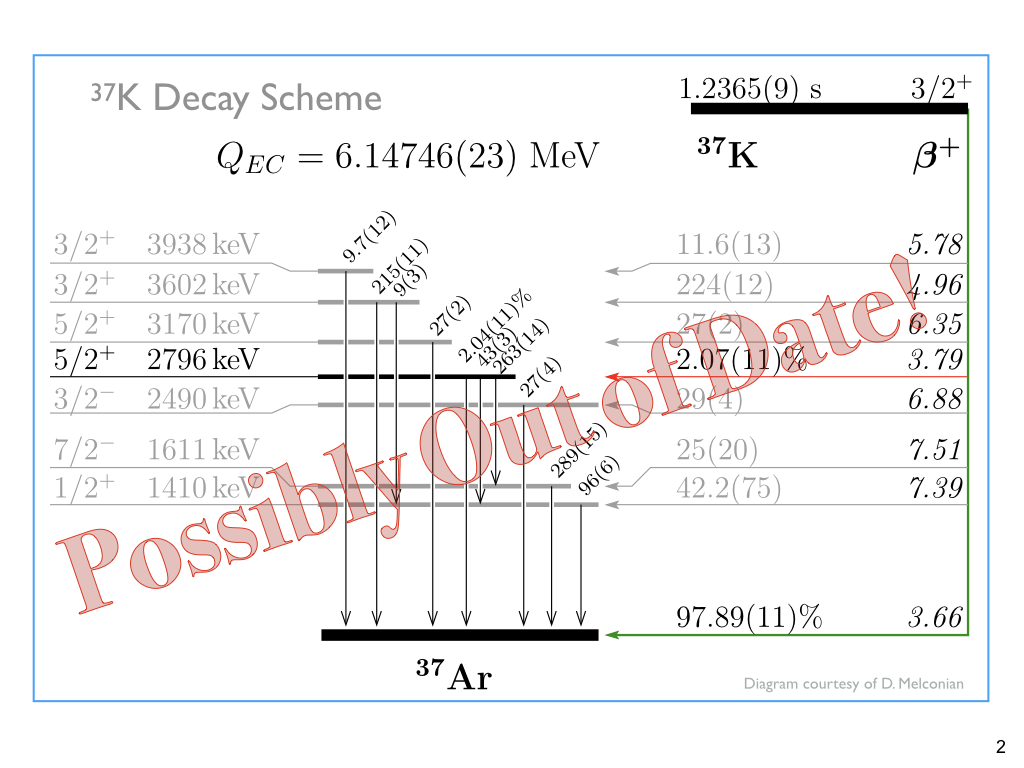
\includegraphics[width=.999\linewidth]
	{Figures/NuclearLevelDiagram_prelim}
	\caption{A level diagram for the decay of $\isotope[37]{K}$.}	
	\label{fig:nuclearleveldiagram}
\end{figure}


\note{Might be worth mentioning about the shake-off electrons too, and how many of them there are.  But then nobody will trust any of the numbers I measured (how did I do that measurement, anyway?), and will want me to just use Dan's that he measured forever ago with a different set of detectors.  (where are those numbers recorded anyway?)  I think I have to mention how many come off and how often at least briefly, because I use the Levinger spectrum for my background modeling.}








%%%% --- * --- %%%%	
\clearpage
\chapter{Atomic Physics Overview}
\label{atomicphysics_chapter}
\section{Magneto-Optical Traps}
	\subsection{Doppler Cooling}
	\subsection{Zeeman Splitting}
	Needs a level diagram.
	\subsection{Atom Trapping with a MOT}

\section{Optical Pumping}
Needs a level diagram.


\section{Shake-off Electron Spectrum}
Shake-off electrons:  where do they come from, and where do they go?  ~\cite{Levinger}.


%%%% --- * --- %%%%	
% !TEX root = ../thesis_main.tex


%%%% --- * --- %%%%	
\clearpage
\chapter{The Experimental Setup}
\label{setup_chapter}

%\color{oldcolor}
\section{Overview and Double MOT System}

The experimental subject matter of this thesis was conducted at TRIUMF using the apparatus of the TRIUMF Neutral Atom Trap (TRINAT) collaboration.  The TRINAT laboratory offers an experimental set-up which is uniquely suited to precision tests of Standard Model beta decay physics, by virtue of its ability to produce highly localized samples of isotopically pure cold atoms within an open detector geometry.  \note{mumble mumble 7ish days of beamtime, mumble mumble 2014.}

The TRINAT lab accepts radioactive ions delivered by the ISAC beamline at TRIUMF.  These ions are collected on the surface of a hot zirconium foil where they are electrically neutralized, and subsequently escape from the foil into the first of two experimental chambers (the ``collection chamber").  Further details on the neutralization process are presented in a previous publication~\cite{gorelov2000}.  Within the collection chamber, atoms of one specific isotope -- for the purposes of this thesis,  \isotope[37]{K} -- are continuously collected into a magneto-optical trap (MOT).  Approximately once per second, the atoms in the collection MOT are transferred to a second experimental chamber (the ``detection chamber'') and loaded into a second MOT (see Fig.~\ref{fig:doublemot}).  Because the transfer and trapping mechanisms rely on tuning to specific atomic resonances, this setup allows for the selection of only a single isotope within the detection MOT, and a significantly reduced background relative to the initial beamline output.  The transfer methodology is discussed in some detail within another publication~\cite{swanson}.

\note{Probably describe the laser transfer method slightly.}  

%The TRIUMF Neutral Atom Trap (TRINAT) offers an experimental set-up which is uniquely suited to precision tests of Standard Model beta decay physics.  Radioactive ions are delivered from the ISAC beamline and neutralized before being trapped in the first of two magneto-optical traps (MOTs).  Approximately once per second, atoms from the first MOT are transferred to the second, where their decay products can be observed with significantly less background than would have been possible in the first trap (see Figure~\ref{fig:doublemot}).  The transfer methodology is discussed in some detail in a paper by Swanson et al~\cite{swanson}. \aside{The point is that this eliminates background from the decays of other stuff.  Or the same stuff.  Stuff that's not centered at the trap.}

\begin{figure}[t!h]
	\centering
	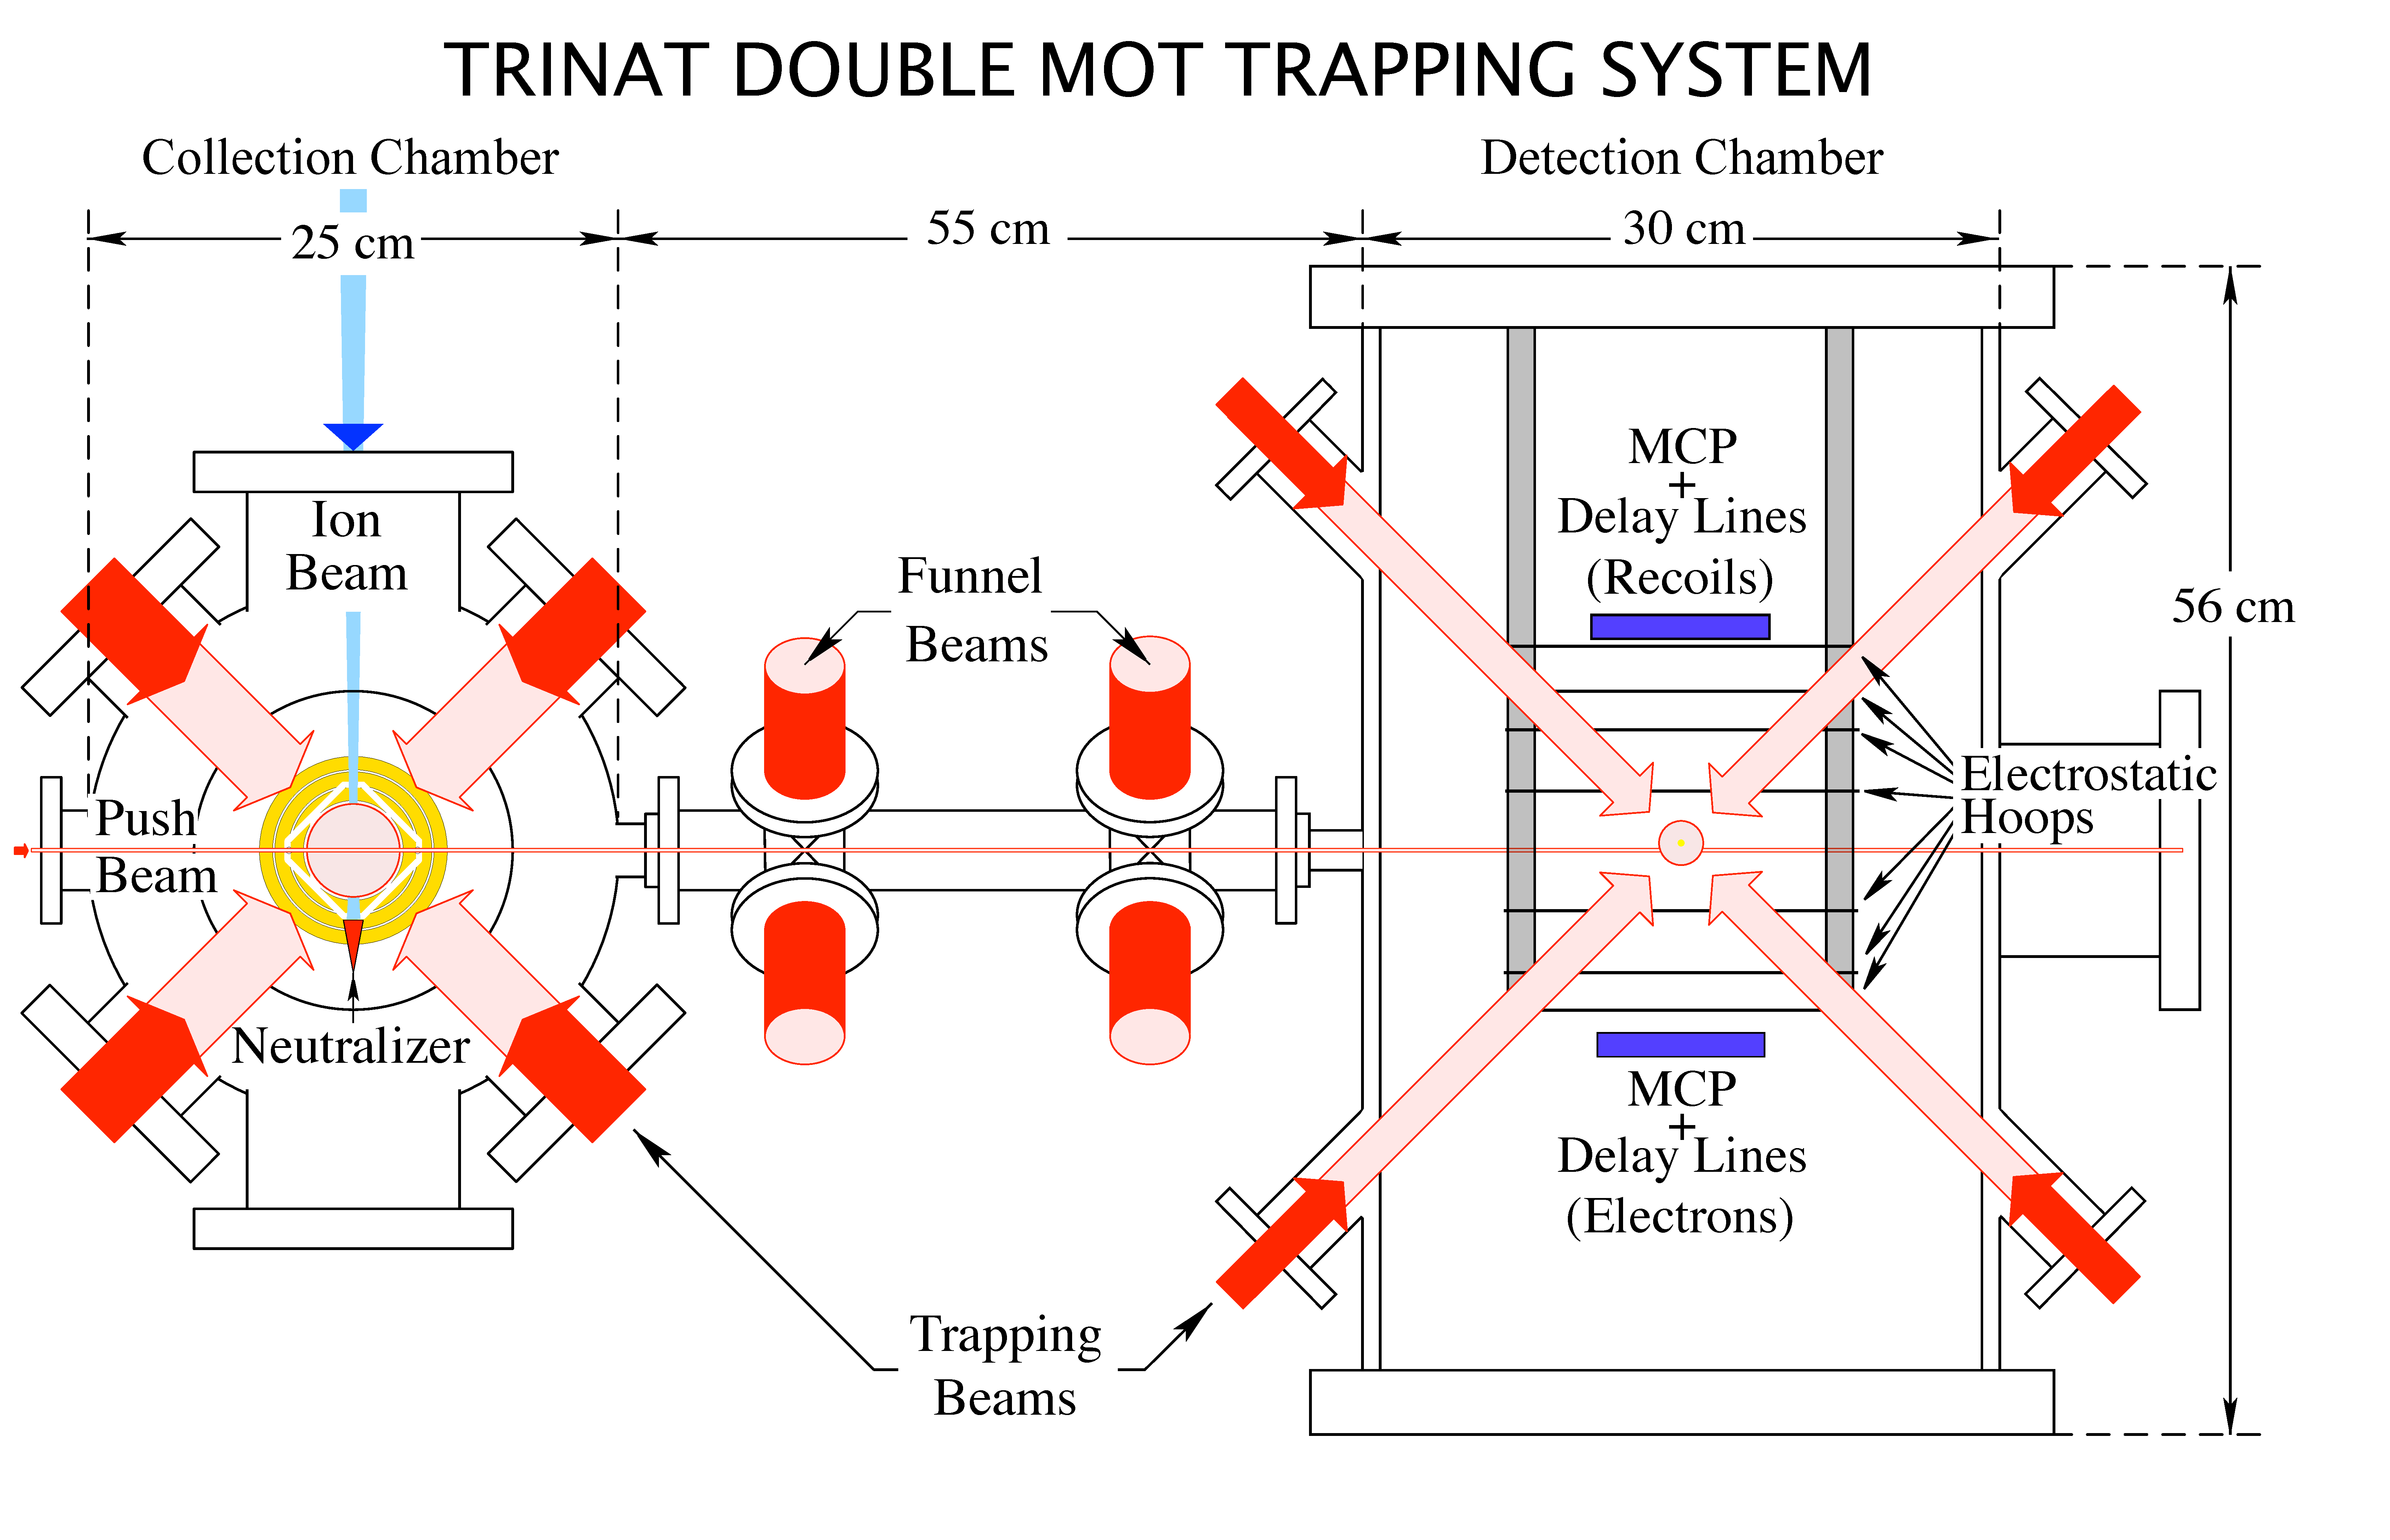
\includegraphics[width=.999\linewidth]
	{Figures/doublemot4.pdf}
	\caption{The TRINAT experimental set-up utilizes a two MOT system in order to reduce background in the detection chamber.}	
	\label{fig:doublemot}
\end{figure}

Once the newly transferred atoms have arrived at the second trap, the MOT cycles 500 times between a state where it is `on' and actively confining atoms to a region of approximately 2\,mm$^3$, to a state where it is `off' and instead the atoms are spin-polarized by optical pumping while the atom cloud expands ballistically before being re-trapped.  This setup is described further in Section~\ref{section:acmot_and_polarization}, and the optical pumping technique and its results are the subject of a recent publication~\cite{ben_OP}.

\note{Below is pretty vague.  I could do better, even for just an overview-summary thing.  Obvs I have to describe it in detail later on *somewhere*, though maybe not in the overview-summary...} 
 
Detectors are positioned about the second MOT for data collection.  The detection chamber 
%(shown in Figure \ref{fig:thechamber}) 
operates at ultra-high vacuum (UHV) and provides not only the apparatus necessary to intermittently confine and then spin-polarize atoms, but also the vbariety of detectors and implements required to quantify their position, temperature, and polarization.  The detection chamber further boasts an array of electrostatic hoops to collect both positively and negatively charged low energy particles into two microchannel plates (MCPs),  and a further set of two beta detectors positioned along the polarization axis, each of which consists of a 40x40 pixel double-sided silicon strip detector (DSSD) and a scintillator and photomultiplier tube (PMT).  The details of the detection chamber setup are described in detail in Section~\ref{section:detectors}.


\section{The AC-MOT and Polarization Setup}
\label{section:acmot_and_polarization}
%\\*
In order to facilitate a measurement of $A_{\mathrm{\beta}}$, we went to great efforts to polarize the atom cloud, and quantify that polarization.  This resulted in a duty cycle in which the atoms were intermittently trapped in the AC-MOT, then optically pumped to polarize them.  While knowledge of the polarization is less critical in a measurement of $b_{\mathrm{Fierz}}$, we still use only the polarized portion of the duty cycle in order to minimize other systematic errors, such as the scintillator energy calibration and overall trap position.

\note{In order to eliminate systematic effects, the polarization direction is flipped every 16 seconds.}

The Magneto-Optical Trap is a well-known technique from atomic physics, used to confine and cool neutral atoms~\cite{raabprentiss}.  The technique is used predominantly with alkalis due to their simple orbital electron structure, and is quite robust, so is appropriate for use with $^{37}\textrm{K}$.  Once set up, the trapping force is specific to the isotope for which the trap has been tuned, which makes it ideal for use in radioactive decay experiments, since the daughters are unaffected by the trapping forces keeping the parent confined.

There are two primary components necessary for any MOT:  a laser, and a magnetic field.  The laser, which must be circularly polarized in the appropriate directions and tuned slightly to the red of an atomic resonance, is split into three perpendicular retroreflected beams, doppler cooling the atoms and (with the appropriate magnetic field) confining them in all three dimensions (see Figure~\ref{fig:mot}).  The TRINAT science chamber includes 6 `viewports' specifically designed to be used for the trapping laser.

\missingfigure{This is going to need another edge-on G4 picture of the chamber to label all the atomic components.  }

\missingfigure{I need \emph{at least} one atomic level diagram.  But possibly as many as 3 level diagrams.  Have to show energies for MOT, energies for OP, and energies for photoionization.  }
\note[color=purple]{JB says:  ``I would say you don't need an atomic level diagram.  You could just describe in words the semiclassical picture of atoms absorbing photons until they are nearly fully polarized, then they stop absorbing.  The optical pulmping + photoionization is then an in situ probe of the polarization. ... You would need to add in words that quantum mechanical corrections to this picture are in the optical Bloch equation approach in B. Fenker et al.  The depolarized states still have high nuclear polarization (1/2 for $F=2, M_F=1$, 5/6 for $F=1, M_F=1$) and determining the ratio of those two populations provides most of the info we need -- we model with the O.B.E, measure the optical pumping light polarization, and float an average transverse magnetic field.  This is adequate to determine the depolarized fraction to 10\% accuracy, which is all that is needed.'' }

\[\]

\note{Is my photoionization description adequate?  ... in light of John's feedback:  no.}
\note[color=jb]{JB says:  ``Since you worked hard on the logic triggers, a photoion spectrum with duty cycle would be appropriate if you want."}

\note{Need to describe how polarization works.}
\note[color=jb]{JB says:  all polarization details could be deferred to ~\cite{ben_OP}.  (be sure to list all authors including [me]).  )}


A MOT also requires a quadrupolar magnetic field, which we generate with two current-carrying anti-Helmholtz coils located within the vacuum chamber itself.  The coils themselves are hollow, and are cooled continuously by pumping temperature-controlled water through them.   

One feature which makes our MOT unusual has been developed as a result of our need to rapidly cycle the MOT on and off -- that is, it is an ``AC-MOT''.  Rather than running the trap with one particular magnetic field and one set of laser polarizations to match, we run a sinusoidal AC current in the magnetic field coils, and so the sign and magnitude of the magnetic field alternate smoothly between two extrema, and the trapping laser polarizations are rapidly swapped to remain in sync with the field~\cite{harveymurray}\cite{thesis}.  See Figure~\ref{fig:acmot}.  

\note{Note that because the atoms within a MOT can be treated as following a thermal distribution, some fraction of the fastest atoms continuously escape from the trap's potential well.  Even with the most carefully-tuned apparatus, the AC-MOT cannot quite match a similar standard MOT in terms of retaining atoms.  The TRINAT AC-MOT has a `trapping half-life' of around 6 seconds, and although that may not be particularly impressive by the standards of other MOTs, it is more than adequate for our purposes.  $^{37}\textrm{K}$ itself has a radioactive half-life of only 1.6 seconds 
(cite someone), so our dominant loss mechanism is radioactive decay rather than thermal escape. }



\note[color=green]{Anyway, here's some figures.  Or possibly one figure.  Whatever.  Also, here's a reference to a figure.  See Fig.~\ref*{fig:themot} (works -- currently ``3.4"), or also its subfigures, eg Fig.~\ref{fig:acmot} (works -- currently ``3.4b") and Fig.~\ref{fig:mot} (works -- currently ``3.4a").  Maybe I have to subref them?  Like, eg, Subfig.~\subref{fig:acmot} (works -- currently ``3.4b") and Subfig.~\subref*{fig:mot} (works -- currently ``3.4a").  What if we try to subref everything?  Consider, eg, Fig.~\subref{fig:themot} (doesn't work).  Yeah, ok, so fortunately the note cites like the text.  This gives an example of shit to do and not to do.  Also, can't do a linebreak within a note.}  

% !TEX root = ../thesis_main.tex

% fig:themot
% 	fig:mot
% 	fig:acmot

\begin{figure}[ht]
	\centering
	\begin{subfigure}[t]{0.242\textwidth}
		\centering
		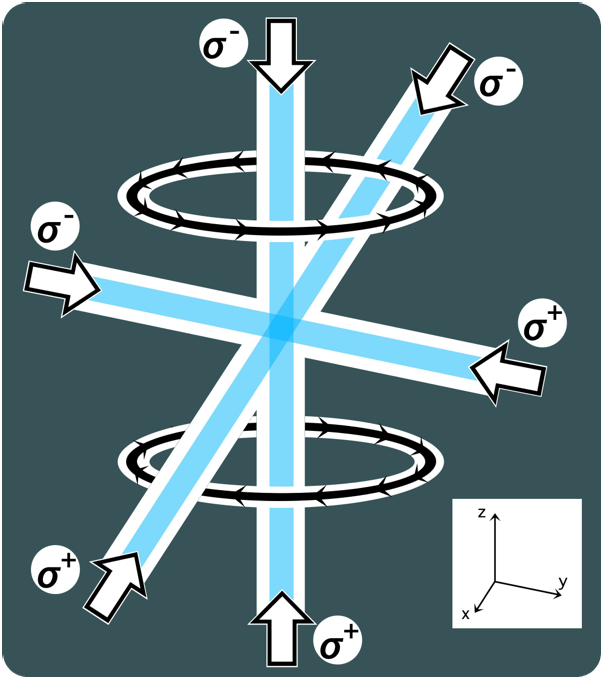
\includegraphics[width=\textwidth]{mot.png}
		\caption{Components of a magneto-optical trap, including current-carrying magnetic field coils and counterpropagating circularly polarized laser beams.}
		\label{fig:mot}
	\end{subfigure}
	\hfill
	\begin{subfigure}[t]{0.728\textwidth}
		\centering
		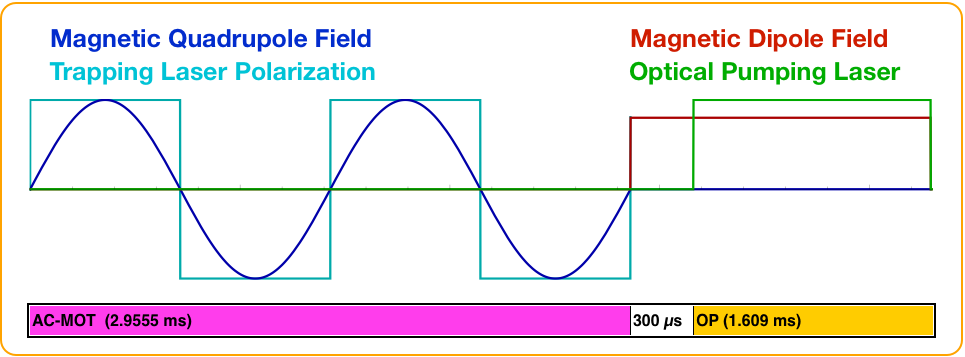
\includegraphics[width=\textwidth]{acmot.png}
		\caption{One cycle of trapping with the AC-MOT, followed by optical pumping to spin-polarize the atoms.  After atoms are transferred into the science chamber, this cycle is repeated 500 times before the next transfer.  The magnetic dipole field is created by running parallel (rather than anti-parallel as is needed for the MOT) currents through the two coils.}
		\label{fig:acmot}
	\end{subfigure}
	\caption{An alternating-current magneto-optical trap with a duty cycle optimized for producing polarized atoms}	
	\label{fig:themot}
\end{figure}

% fig:themot
% 	fig:mot
% 	fig:acmot



We spin-polarize $^{37}\textrm{K}$ atoms within the trapping region by optical pumping~\cite{ben_OP}.  A circularly polarized laser is tuned to match the relevant atomic resonances, and is directed through the trapping region along the vertical axis in both directions.  When a photon is absorbed by an atom, the atom transitions to an excited state and its total angular momentum (electron spin + orbital + nuclear spin) along the vertical axis is incremented by one unit.  When the atom is de-excited a photon is emitted isotropically, 
%\comment{(is it still isotropic when it's polarized?  I bet it's not.)}
so it follows that if there are available states of higher and lower angular momentum, the \emph{average} change in the angular momentum projection is zero.  If the atom is not yet spin-polarized, it can absorb and re-emit another photon, following a biased random walk towards complete polarization.  

%\missingfigure{Need a picture of the whole duty cycle.  Possibly combine with ~\ref{fig:acmot}.}
\begin{figure}[h!!t]
	\centering
	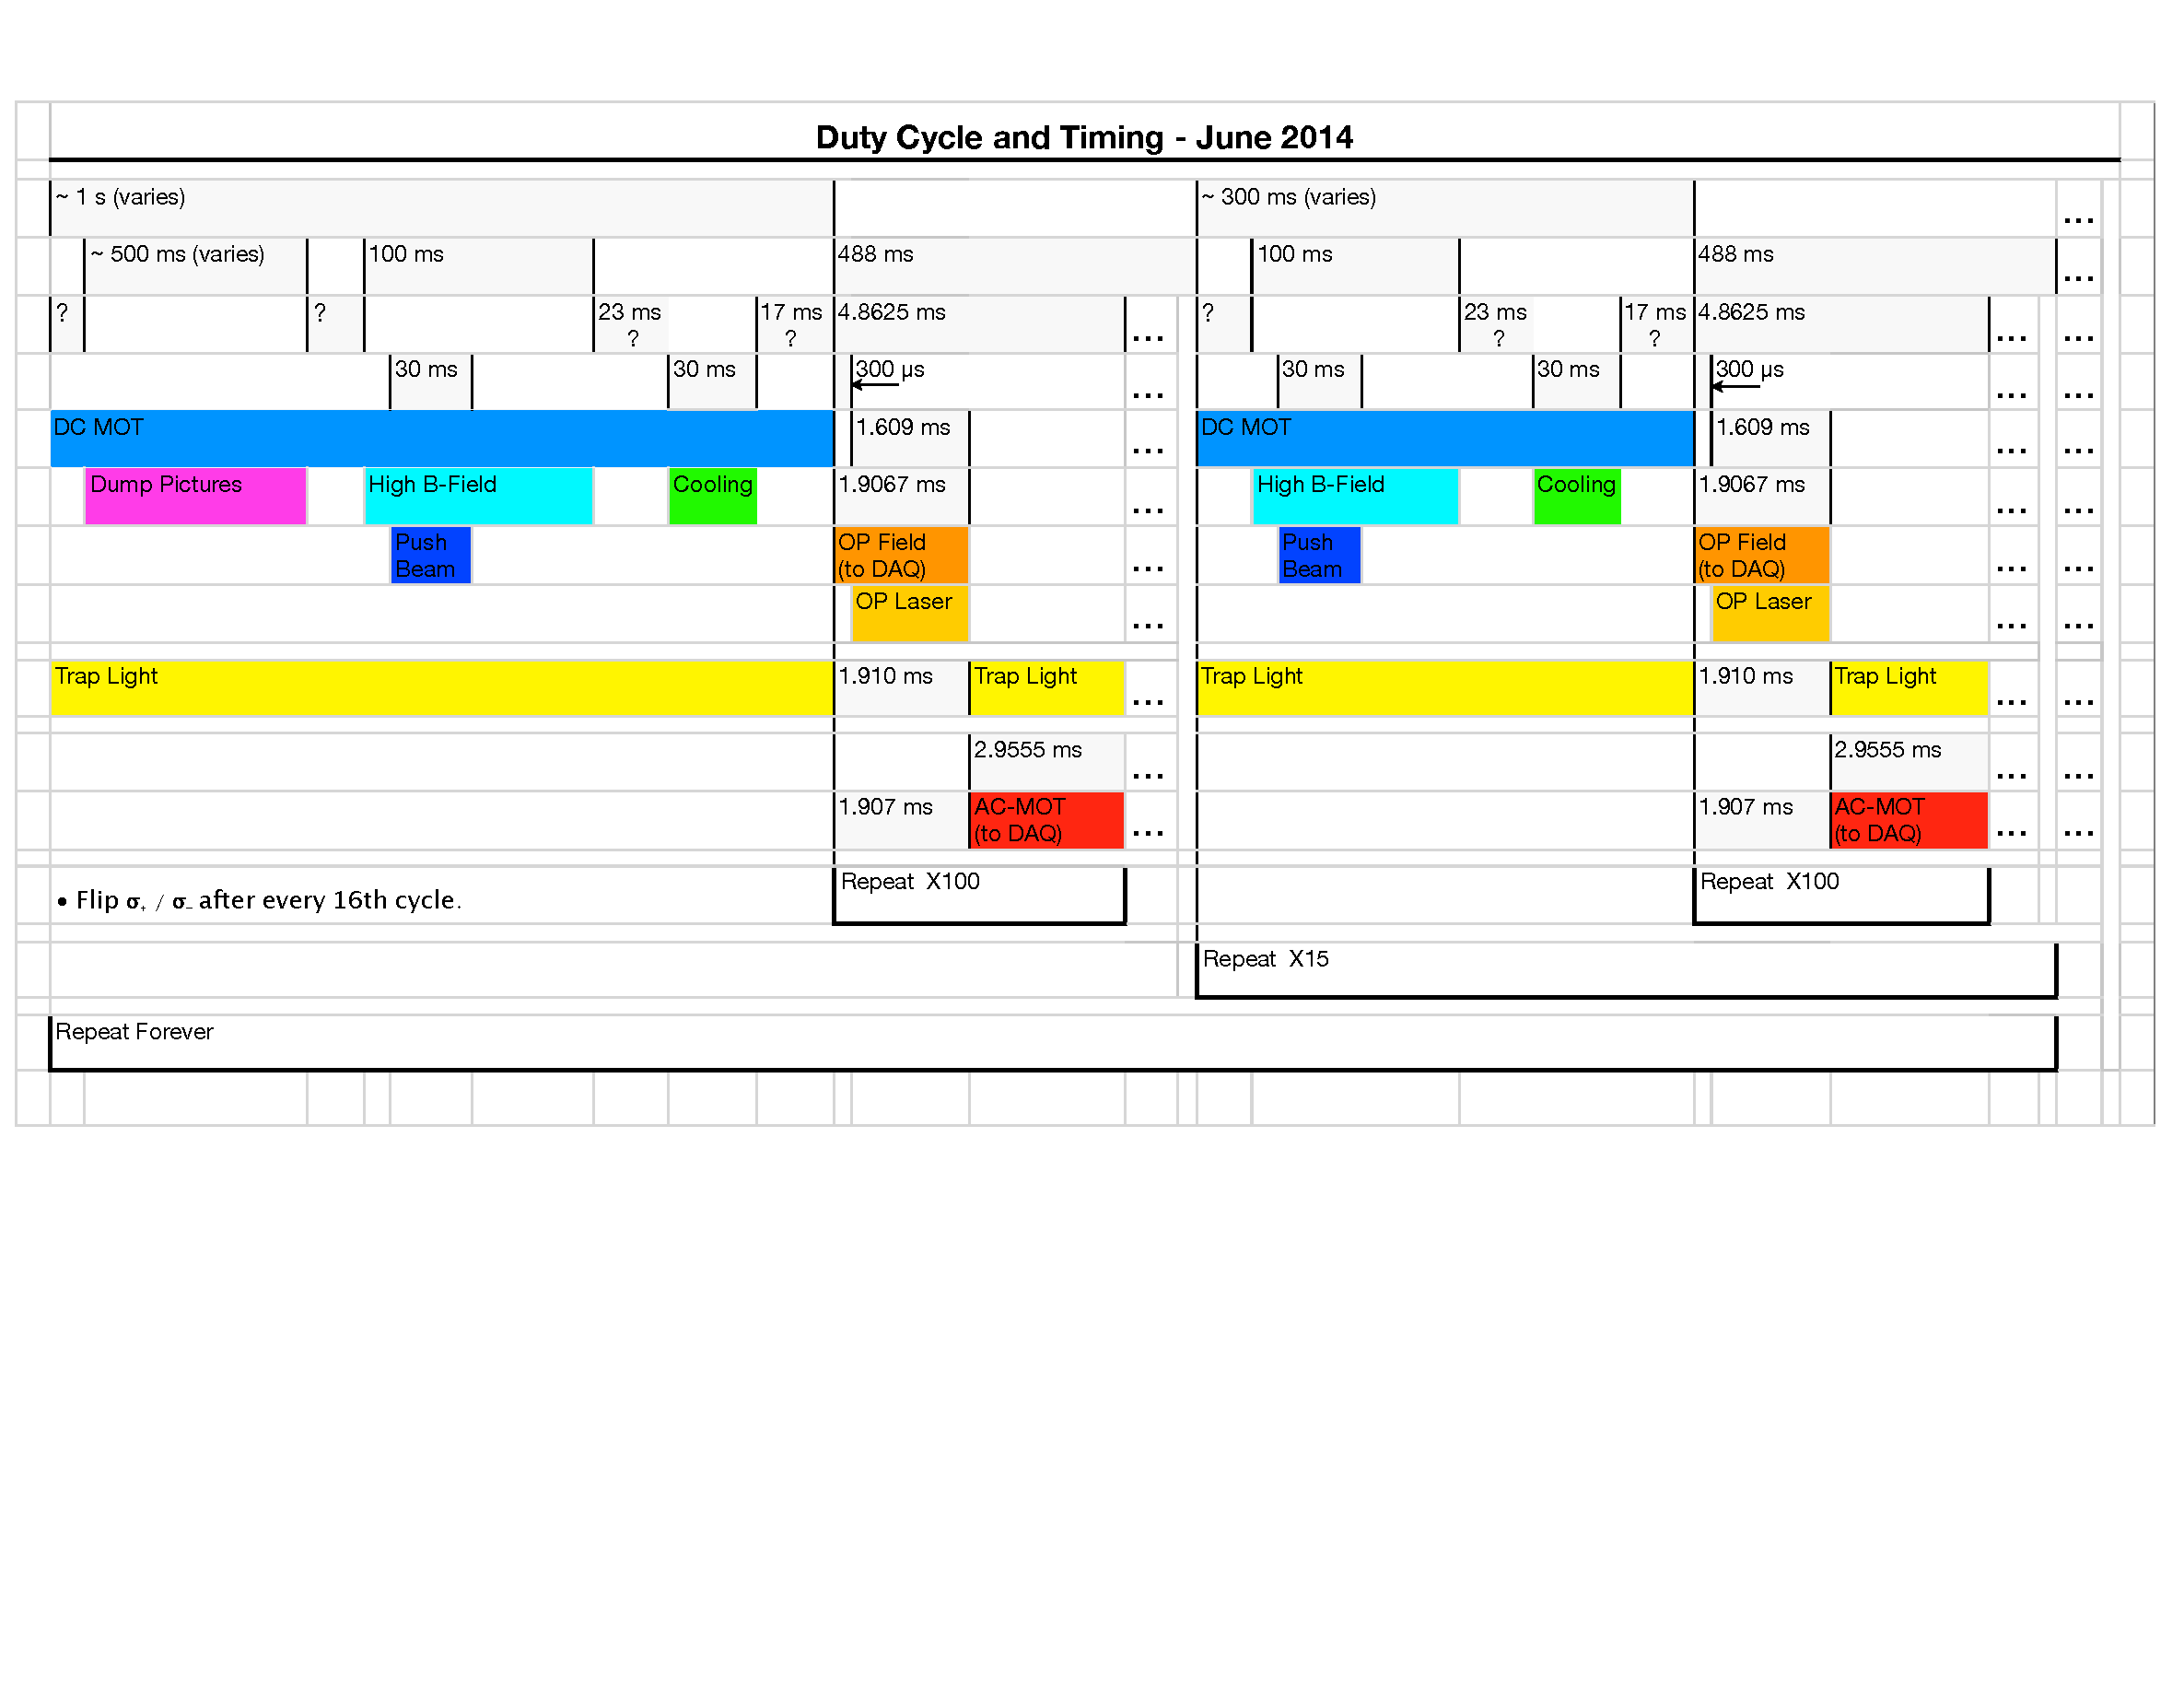
\includegraphics[width=.999\linewidth]
	{Figures/DutyCycle_2014.pdf}
	\caption{The duty cycle used for transferring, cooling, trapping, and optically pumping $\isotope[37]{K}$ in 2014.}	
	\label{fig:dutycycle}
\end{figure}


In order to optimally polarize a sample of atoms by this method, it is necessary to have precise control over the magnetic field.  This is because absent other forces, a spin will undergo Larmor precession about the magnetic field lines.  In particular, the magnetic field must be aligned along the polarization axis (otherwise the tendency will be to actually depolarize the atoms), and it must be uniform in magnitude over the region of interest (otherwise its divergencelessness will result in the field also having a non-uniform direction, which results in a spatially-dependent depolarization mechanism).  Note that this type of magnetic field is not compatible with the MOT, which requires a linear magnetic field gradient in all directions (characteristic of a quadrupolar field shape), and has necessitated our use of the AC-MOT as described in Section~\ref{section:acmot_and_polarization}.\aside{that's this section.  I should really describe the AC-MOT.}



%\color{black}
%	\subsection{\textbf{Nuclear Setup}}
\section{Measurement Geometry and Detectors}
\label{section:detectors}
\note{Do I want to make an entirely new section for the MCPs and electric field stuff?  It doesn't seem to quite fit in either of the two sections here...}
	Needs several diagrams.  Back-to-back beta detectors along the polarization axis.  Back-to-back MCPs in an electric field to tag events from the trap, and to measure the trap position and polarization.  Hoops to produce the electric field.  Many laser ports to make the MOT functional, and for optical pumping.  Fancy mirror geometry to combine optical pumping and trapping light along the vertical axis.  Water-cooled (anti-)Helmholz coils within the chamber for the AC-MOT, fast switching to produce an optical pumping field.  
%	\subsection{\textbf{All the Detectors}}


% !TEX root = ../thesis_main.tex


% "fig:thechamber"

\begin{figure}[h!!!tb]
	\centering
%	\hspace*{\fill}%
	\subfloat[A decay event within the TRINAT science chamber.  After a decay, the daughter will be unaffected by forces from the MOT.  Positively charged recoils and negatively charged shake-off electrons are pulled towards detectors in opposite directions.  Although the $\beta^+$ is charged, it is also highly relativistic and escapes the electric field with minimal perturbation.
	%\comment{The pic is still kind-of fuzzy.}
	]
	{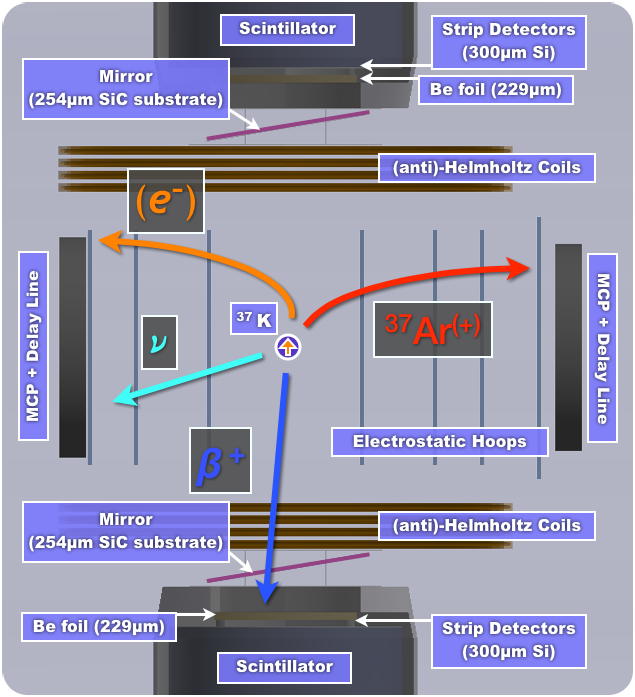
\includegraphics[width=.530\linewidth]{Figures/chamber_decayevent3.png}\label{chamber_decayevent} }
	\hspace*{\fill}
%	\hfill
	\hspace*{\fill}
	\subfloat[Inside the TRINAT science chamber.  This photo is taken from the vantage point of one of the microchannel plates, looking into the chamber towards the second microchannel plate.  The current-carrying copper Helmholtz coils and two beta telescopes are visible at the top and bottom.  The metallic piece near the center is one of the electrostatic `hoops' used to generate an electric field within the chamber.  The hoop's central circular hole allows access to the microchannel plate, and the two elongated holes on the sides allow the MOT's trapping lasers to pass unimpeded at an angle of 45 degress `out of the page'.]	
	{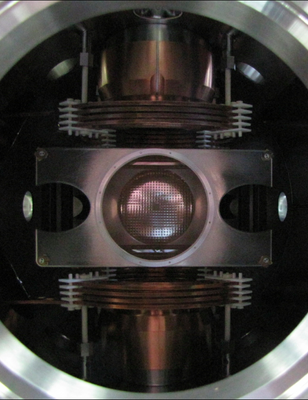
\includegraphics[width=.444\linewidth]{Figures/chamber_photo_2.png}}
%	\hspace*{\fill}%
	\caption{The TRINAT detection chamber}	
	\label{fig:thechamber}
\end{figure}


% "fig:thechamber"




\note{...(shown in Figure \ref{fig:thechamber}) ...}
The beta detectors, located above and below the atom cloud along the axis of polarization (see Figure~\ref{chamber_decayevent}), are each the combination of a plastic scintillator and a set of silicon strip detectors.  Using all of the available information, these detectors are able to reconstruct the energy of an incident beta, as well as its hit position, and provide a timestamp for the hit's arrival.  Together the upper and lower beta detectors subtend approximately 1.4\% of the total solid angle as measured with respect to the cloud position. 

It must be noted that the path between the cloud of trapped atoms and either beta detector is blocked by two objects:  a 275$\,\mu$m silicon carbide mirror (necessary for both trapping and optical pumping), and a 229$\,\mu$m beryllium foil (separating the UHV vacuum within the chamber from the outside world).  In order to minimize beta scattering and energy attenuation, these objects have had their materials selected to use the lightest nuclei with the desired material properties, and have been manufactured to be as thin as possible without compromising the experiment.  As the $^{37}\textrm{K} \rightarrow \,^{37}\textrm{\!Ar} + \beta^{+} + \nu_e$ decay proceess releases $Q=5.125$\,MeV of kinetic energy~\cite{Q_value}, the great majority of betas are energetic enough to punch through both obstacles without significant energy loss before being collected by the beta detectors.  

On opposing sides of the chamber, and perpendicular to the axis of polarization, two stacks of $\sim$ 80\,mm diameter microchannel plates (MCPs) have been placed (see Figure~\ref{fig:thechamber}) as detectors, providing a time stamp when a particle is incident on their surfaces.  Behind each stack of MCPs there is a set of delay lines, which provide  position sensitivity for these detectors.   

In order to make best use of these MCPs, we create an electric field in order to draw positively charged particles into one MCP, while drawing negatively charged electrons into the other MCP.  Seven electrostatic hoops have been placed within the chamber (see Figure~\ref{fig:thechamber}), and are connected to a series of high voltage power supplies.  See Sections~\ref{photoions} and~\ref{pos_recoils} for a discussion of what sort of charged particles we expect to observe in these detectors and how they are created.  
  
Scientific data has been collected at field strengths of 395 V/cm, 415 V/cm, and 535 V/cm.  It should be noted that these field strengths are too low to significantly perturb any but the least energetic of the (positively charged) betas from the decay process, and these low energy betas would already have been unable to reach the upper and lower beta detectors due to interactions with materials in the SiC mirror and Be foil vacuum seal.  




%%%% --- * --- %%%%	
% !TEX root = ../thesis_main.tex



%%%% --- * --- %%%%	
\clearpage	
\chapter{Calibrations}
\label{calibrations_chapter}
	
%\section{Polarization}
%	%\\*
%	Polarization measurement was conducted on a different set of data, collected in between the measurements used for $A_{\mathrm{\beta}}$ and $b_{\mathrm{Fierz}}$, and at a higher electric field, because we were unable to run both our MCP detectors simultaneously.  
%	
%\section{Trap Position}
%	%\\*
%	Measured using the same dataset that was used to quantify the polarization.  The trap drifts slightly over the course of our data collection.  Describe the rMCP calibration needed to extract this info.  
%

\section{Cloud Measurements via Photoionization}
\label{cloud}
\label{photoions}
In order to measure properties of the trapped $^{37}\textrm{K}$ cloud, a 10\,kHz pulsed laser at 355\,nm is directed towards the cloud.  These photons have sufficient energy to photoionize neutral $^{37}\textrm{K}$ from its excited atomic state, releasing 0.77\,eV of kinetic energy, but do not interact with ground state $^{37}\textrm{K}$ atoms.  The laser is of sufficiently low intensity that the great majority of excited state atoms are \emph{not} photoionized, so the technique is only very minimally destructive.  

Because an electric field has been applied within this region (see Section~\ref{field}) the $^{37}\textrm{K}^+$ ions are immediately pulled into the detector on one side of the chamber, while the freed $e^-$ is pulled towards the detector on the opposite side of the chamber.  Because  $^{37}\textrm{K}^+$ is quite heavy relative to its initial energy, it can be treated as moving in a straight line directly to the detector, where its hit position on the microchannel plate is taken as a 2D projection of its position within the cloud.  Similarly, given a sufficient understanding of the electric field, the time difference between the laser pulse and the microchannel plate hit allows for a calculation of the ion's initial position along the third axis.  

With this procedure, it is possible to produce a precise map of the cloud's position and size, both of which are necessary for the precision measurements of angular correlation parameters that are of interest to us here.  However, it also allows us to extract a third, slightly more subtle and significantly more important measurement:  the cloud's \emph{polarization}.

The key to the polarization measurement is that only atoms in the excited atomic state can be photoionized.  While the MOT runs, atoms are constantly being pushed around and excited by the trapping lasers, so this period of time provides a lot of information for characterizing the trap size and position.  When the MOT is shut off, the atoms quickly return to their ground states and are no longer photoionized until the optical pumping beam is turned on.  As described in Section~\ref{op}, and in greater detail in~\cite{ben_OP}, the optical pumping process involves repeatedly exciting atoms from their ground states until the atoms finally cannot absorb any further angular momentum and remain in their fully-polarized (ground) state until they are perturbed.  Therefore, there is a sharp spike in excited-state atoms (and therefore photoions) when the optical pumping begins, and none once the cloud has been completely polarized.  The number of photoion events that occur once the sample has been maximally polarized, in comparison with the size and shape of the initial spike of photoions, provides a very precise characterization of the cloud's final polarization~\cite{ben_OP}.

\note{Trap position -- Measured using the same dataset that was used to quantify the polarization.  The trap drifts slightly over the course of our data collection.  Describe the rMCP calibration needed to extract this info.}
\note{Polarization measurement was conducted on a different set of data, collected in between the measurements used for $A_{\mathrm{\beta}}$ and $b_{\mathrm{Fierz}}$, and at a higher electric field, because we were unable to run both our MCP detectors simultaneously.  }

\section{Beta Detectors}
	%\\*
	Energy calibration for the scintillator+PMT setup changed dramatically at one point.    Describe how calibration was done.  Also describe how the DSSD calibration was done, even though it wasn't implemented by me.  
	
\section{The eMCP}
	%\\*
	I can describe the eMCP calibration here, even though it mostly wasn't implemented by me.  It is tangentially relevant to data selection and background estimation by providing an experimental energy spectrum for shake-off electrons.  




%%%% --- * --- %%%%
% !TEX root = ../thesis_main.tex


%%%% --- * --- %%%%
\clearpage	

\chapter{The Experimental Signature}
\label{signature_chapter}

%\section{}
\note{Possibly this can be combined with the ``Background and Motivation'' or ``Theory'' chapters?  Why do I even *have* two of those chapters, if not for this? Anyway, surely I don't need *three* of them...}
\section{General Stuff}
\comment{The point is, the presence of either scalar or tensor interactions will produce a $\bFierz$ term in the decay PDF.  It has other effects on the PDF, but those come in at higher-order in the tiny scalar and tensor couplings.  So, the Fierz term would be by far the biggest thing that changes in the PDF.  The PDF describes the energy and momentum of the outgoing beta w.r.t. a variety of other things.  Notably, we can write an elegant-ish description of beta momentum w.r.t. nuclear polarization direction, and ignore the neutrino completely after integrating over it.  We have a PDF in beta \emph{direction} (w.r.t. polarization), and beta \emph{energy}.  To lowest order (and lowest order is best order) the distribution w.r.t. polarization direction doesn't change, but the distribution w.r.t. energy does change.  Or ... something?  The point is, it makes a change in the beta energy spectrum.  This change is most pronounced at low energies, because the Fierz term is scaled by $(1/\Ebeta)$.  However, the asymmetry is also a function of $\Ebeta$.  A different function of $\Ebeta$.  In fact, it is scaled by $(\pbeta/\Ebeta)$ within the PDF, which is distinctly different than $\bFierz$.  So, one might ask what effect a $\bFierz$ term would produce on a constructed asymmetry spectrum.  ....This explanation has gone way off track.}


\section{TBD}
\note[color=jb]{JB:  You need to at some point say that the supersum is the beta energy spectrum.  There are experiments trying to do this method better, but they are very difficult.  UCNA published a combined energy spectrum and Abeta[Ebeta] analysis on the neutron in March 2020~\cite{NeutronbFierz_March2020}.}
\note{I can't help but also notice the follow-up article from September 2020~\cite{NeutronbFierz_September2020}.  Ugh. }
I really need an excuse to include more pictures of data.  Also, more pictures of simulations.

\missingfigure{Show individual beta energy spectra.  ...with a variety of different cuts, perhaps?}

\missingfigure{Show simulated spectra separated by scattering category.}

\missingfigure{Show SimpleMC spectra, show the supersum, show the superratio, show the superratio asymmetry.  Maybe do some simple fits to show how much better the superratio asymmetry is than \emph{not} the superratio asymmetry.  }


\section{The Superratio and Asymmetry}
%\\*
The data can be combined into a superratio asymmetry.  This has the benefit of causing many systematics to cancel themselves out at leading order.  It also will increase the fractional size of the effects we're looking for.  This can be shown by using math.  

\section{Signature of a Fierz Term in This Experiment}
%\\*
Not all systematics effects are eliminated.  We'll want to be careful to propagate through any effects that are relevant.  Using the superratio asymmetry as our physical observable makes this process a bit messier for the things that don't cancel out, but it's all just math.  

\section{Comparative Merits of the Superratio and Supersum for Measurement}
%\\*
Some other groups have performed similar measurements using the supersum as the physical observable.  There are pros and cons to both methods.  I can show, using a back-of-the-envelope calculation, that for this particular dataset, the superratio asymmetry method produces a better result.  

\begin{figure}[h!!t]
	\centering
	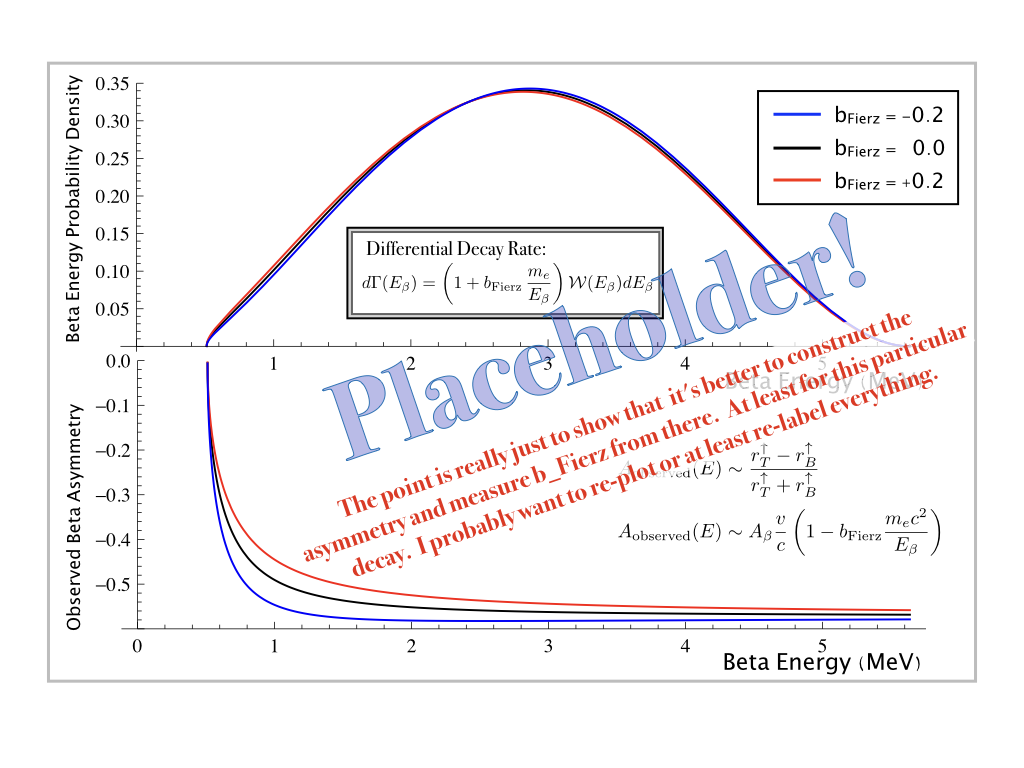
\includegraphics[width=.999\linewidth]
	{Figures/SuperSumSuperRatio_prelim}
	\caption{Here's why it's better to extract $\bFierz$ from an asymmetry, in this case.}	
	\label{fig:supersumsuperratio}
\end{figure}





%%%% --- * --- %%%%
% !TEX root = ../thesis_main.tex
%
%
%
%%%% --- * --- %%%%	
\clearpage
\chapter{Analysis}
\label{analysis_chapter}
\note[color=org]{from JB, on whether to combine `Analysis' chapter with `Calibrations' chapter:  ``I see no special reason either way.  I would say the topics seem distinct.''}
%
\note[color=jb]{JB says:  ``ch 7 (now ch.6) ((Ch.5)) looks fine to me.''  ...even in spite of the giant paragraph suggestions below, I guess.}
%\note[color=org]{Do I actually want to combine this with Chapter~\ref{calibrations_chapter}?}
%\note[color=org]{from JB:  you ask at the start if you should combine it (Ch.7 (now Ch.6) ((Ch.5)), `Analysis') with Ch.6 (now Ch.5) `Calibrations'. I see no special reason either way.  I would say the topics seem distinct.}
\note[color=jb]{John proposes an intro statement for this chapter.  The following two paragraphs are a direct quote from him:}

%\note[color=jb]{JB:  Here is what I suggest for the intro the Analysis section:  (n.b.:  at the time of this comment, that was Ch.7)
%\\...\\
%7.0
\comment{
Analysis is critical to a precision measurement, as most of the research is in
determining systematic uncertainties by self-consistent analysis and simulations.
Each detector in this experiment is critical and has independent calibrations and cuts.
Full explanation is here (and in two following chapters) justifying choice of the deterministic cuts,
because in the analysis in this thesis the data was not blinded.
The main goal of blinding was nevertheless achieved-- to make sure all analysis is done
completely with full redundancy of checks wherever possible-- so the discipline entailed must
be described in full detail.
Here there are details of detectors:
eMCP
rMCP
beta DSSD
scintillator.
%\\...\\

The collaboration has done an independent analysis fixing bFierz to zero.
Differences with that analysis are interleaved in this section.
Critical physics improvements concern
an emcp-beta timing walk correction which enabled an improved cut against background, also incorporating
a more complete modelling of decay backgrounds from untrapped atoms.
Technical corrections include a correct treatment of the polarization cycle.
An arbitrary change in the deltaE radius cut is kept self-consistent.
}
%\\...\\
%Then Section 7.1...
%}

%\section{Data Selection and Pre-Processing}
%\section{Run Parameters and Preliminary Cuts}
\section{Data Selection and Preliminary Cuts}
Although the detection chamber was designed to feature two MCP detectors on opposing sides of an applied electric field intended for simultaneous use (see Section~\ref{section:mcps}), % to collect positively charged recoiling ions on the rMCP and negatively charged shake-off electrons on the eMCP 
in practice the two detectors produced quite a bit of feedback when operated at the same time.  In order to salvage usable data from the beamtime, we ended up running only one detector at a time, but switched which detector was in use every few hours, collecting approximately the same amount of data with each detector.  Thus, the runs are sorted into `electron' and `recoil' runs, depending on what the detector in use was intended to detect.  

While the beta asymmetry and Fierz interference are best evaluated using the electron runs, the recoil runs are best for evaluating the polarization (a dominant uncertainty in the beta asymmetry measurement) and the cloud position.  The polarization measurement is the subject of a recent publication (see~\cite{ben_OP}), and the cloud position evaluation is discussed in more detail in Chapter~\ref{calibrations_chapter}.

The data is further split up into four runsets:  A, B, C, and D based on when certain detection settings were adjusted, and each of these runsets contains both electron and recoil runs.  These four runsets were then treated separately for nearly all parts of the analysis.  In particular, Data Set A was neglected completely during analysis after it was determined that one scintillator had an improperly set hardware threshold such that lower energy betas weren't being detected at all.  Additionally, there was a QDC module failure between Runsets B and C, resulting in an abrupt change in calibration for the two scintillators.  
\note{`The observant reader may find it curious that the listed runsets start at ``B'' and continue alphabetically.  There was initially a ``Runset A'' collected as well, however it was determined later that this data could not be salvaged for use in the final analysis because one of the scinitillators had its hardware threshold set above the compton peak, and without that reference point an accurate calibration could not be performed.'}

%\note{Also, the background was too noisy in Set A I think.  Also, pretty sure there isn't really that much data in Set A at all.  Also-also, Set A has E=66.7, so can't use it for more stats on the other backgrounds. ... Maybe I should just look up what the deal even was with Set A, since I don't really remember.} 

%\note{What did I change between Runsets B and C?  Between Runsets C and D?  ...OP time, yes, but also and one point a PMT(?) (eta:  it was a QDC) blew out and we replaced it, so then the scintillator calibration was a bit different afterward.  Anyway, I should maybe just make a goddamn table.  Table goes here.}

% !TEX root = ../thesis_main.tex


\begin{table}[h!!!!t]
	\begin{center}
	\begin{tabular}{ c || p{5cm} | p{5cm} | p{1.2cm} | }
			\multicolumn{1}{  c  }{ } & 
				\multicolumn{1}{  c  }{ \!\!Electron Runs\!\! } &  \multicolumn{1}{   c  }{ Recoil Runs }  &  \multicolumn{1}{   c  }{ OP Delay }  \\
			\cline{2-4}
			\multirow{1}{*}{Runset A}	& 314, 362, 363, 383, 384, 385, 386, 393, 420.
									%	& 303, 308, 309, 310, 311, 312, 313, 318, 326, 327, 328, 340, 342, 343, 361, 368, 370, 371, 376, 377, 378, 394, 395, 396, 398, 399, 400, 401, 402, 409, 410, 411, 412, 413, 414, 415, 416, 417, 418, 419.
										& 303, 308-313, 318, 326, 327, 328, 340, 342, 343, %361, 368, 370, 371, 
										376, 377, 378, 394, 395, 396, 398-402, 409-419.
										& $300\,\mu s$
										\\
			\cline{2-4}
			\multirow{1}{*}{Runset B}	& 428-437, 440-445.
										& 421-426, 446, 447, 449.
										& $300\,\mu s$
										\\
			\cline{2-4}
			\multirow{1}{*}{Runset C}	& 476, 477.
										& 450, 454, 455, 460-466, 473, 474.
										& $700\,\mu s$
										\\
			\cline{2-4}
			\multirow{1}{*}{Runset D}	& 478-489, 502, 503, 504, 505, 510, 513.
										& 491, 497, 498, 499, 509.   
										& $400\,\mu s$
										\\
			\cline{2-4}
	\end{tabular}
	\end{center}
	\note{MUST check to make sure I didn't use Run 420 in ``good runs" in the end!!!}
	\note{I have more (really early) runs classed in Set A than Ben had.  In the end, we didn't use them so it doesn't matter.  But...what?}
	\note{Ugh.  My categorization system is slightly different than Ben's on the later recoils.  That's annoying.}
	\note{Other things I could list here:  Electric field strengths, total runtime.}
	\caption[List of Runs]{A list of 2014 online runs with potentially usable data.  Runset A was discarded completely due to problems with hardware threshold settings.  There was a QDC module failure before Run 450, so it and all subsequent runs were performed using a different module, and as a result the scintillator calibrations changed slightly at this time.  Anyway, the point of this thing is to show which electron runs and recoil runs go together, for the purposes of evaluating polarization and cloud attributes.}
	\label{table:runlist}
\end{table}


% !TEX root = ../thesis_main.tex


\begin{table}[h!!!!tb]
	\begin{center}
	\begin{tabular}{ c || p{1.2cm} | r | l | p{5.8cm} | }
		\multicolumn{4}{l}{Electron Runs} %& \multicolumn{1}{l}{Electron Runs} 
		\\
		\cline{1-3}
		\multicolumn{5}{c}{ }
		\\
			\multicolumn{1}{  c  }{ } & 
				\multicolumn{1}{  c  } { \!\!OP Delay\!\! } &  \multicolumn{1}{ c }{ \!\!Events\!\! }  
				& \multicolumn{1}{ c }{ \!\!Electric Field\!\! } & \multicolumn{1}{ c }{ Runs } 
				\\
			\cline{2-5}
			\multirow{1}{*}{Runset A}	& $300\,\mu s$
										& 0
										& \,\,\,$66.67$ V/cm
										& 314, 362, 363, 383-386, 393. %, 420.
										\\
			\cline{2-5}
			\multirow{1}{*}{Runset B}	& $300\,\mu s$
										& 173,640
										& $150.0$\,\, V/cm
										& 428-437, 440-445.
										\\
			\cline{2-5}
			\multirow{1}{*}{Runset C}	& $700\,\mu s$
										& 18,129
										& $150.0$\,\, V/cm
										& 476, 477.
										\\
			\cline{2-5}
			\multirow{1}{*}{Runset D}	& $400\,\mu s$
										& 207,596
										& $150.0$\,\, V/cm
										& 478-489, 502-505, 510, 513.
										\\
			\cline{2-5}
	\end{tabular}
	\end{center}
	\note{A list of 2014 online runs with potentially usable data.  Runset A was discarded completely due to problems with hardware threshold settings.  There was a QDC module failure before Run 450, so it and all subsequent runs were performed using a different module, and as a result the scintillator calibrations changed slightly at this time.  Anyway, the point of this thing is to show which electron runs and recoil runs go together, for the purposes of evaluating polarization and cloud attributes.}
	\note{Ben doesn't seem to include Runs 436 and 437 in *any* set of good runs.  Is it an oversight?  I think they're perfectly legit electron runs.  They're fairly long runs...}
	\caption[List of Electron Runs]{A list of electron runs and associated parameters.  The ``Events'' column includes only the number of events that passed all cuts.}
%	\note{This table might eventually go away.  Mostly I just want a record of the total `good' counts.  In total, $N=399,365$.}
	\label{table:runlist_electrons}
\end{table}



Before proceeding further, several basic cuts are performed on the data.  For the Electron Runs which are to be processed directly into a physical measurement, we consider only events in which there was a recorded hit \emph{both} on the eMCP \emph{and} on (at least) one of the scintillators.  The required scintillator hit, of course, is potentially a beta, and so it is obvious why this must be present.  The eMCP hit requirement -- particularly with the timing of the eMCP hit occuring within a certain time range relative to the scintillator hit -- is used to tag beta decay events originating from the cloud, as opposed to those originating from some other surface within the chamber.  The precise time interval to be used, and how its results should be evaluated,\aside{also discussed: how we decide what counts as an eMCP hit at all} is discussed in Section~\ref{section:emcp_cuts}, but for the first pass through the data it is good enough to simply require that an eMCP hit occurred.\aside{Awkward stupid phrasing.}  Although not every beta decay event from the cloud will produce a hit on the eMCP, this requirement eliminates a great deal of background that would otherwise be challenging to evaluate.  \aside{Also, we claim that it doesn't bias the data.  Much.  Didn't I try to evaluate how much it biased the data at one point?}  
 
%The scintillator hit is considered to be potentially a beta from a decay
Because the eMCP hit is required as a `tag' of good events, it is also necessary to remove from direct consideration any event which is coincident with a pulse of the photoionization laser.  When photoionization occurs within the atom cloud, an orbital electron is removed from the atom and will be accelerated by the electric field into the eMCP, just as a shake-off electron from a decay might be.  If, by chance, this photoelectron arrives in coincidence with a scintillator hit, it would be interpreted as a decay event from the trap -- unless we preemtively discard it.  


Over the course of the runtime, there were several instances where we noted an apparent electrical discharge within the experimental chamber, producing enormous backgrounds for a short time.  The detectors typically recovered quickly afterward, so it was neither necessary nor useful to stop an entire run to wait for the system to recover.  Instead, the time when the discharge occurred was recorded, and events within approximately one minute of the spark time were discarded.  

%Because it is of the utmost importance to understand the nuclear spin-polarization immediately prior to a decay, 
We use only the ``fully polarized'' events for which we have a detailed understanding of the nuclear polarization (described in more detail in ~\cite{ben_OP}).  This means we must use \emph{only} events from the ``optical pumping'' portion of the duty cycle (see Fig.~\ref{fig:dutycycle}), and discard events when the DC- or AC-MOT is active.  After the AC-MOT is shut off, there is a short delay before optical pumping begins (see Table~\ref{table:runlist}) to allow the magnetic field to decay, and it is only after $100\,\mu s$ of optical pumping that we consider the atoms to be fully polarized.  Furthermore, because the magnetic field from the DC-MOT is slow to decay (relative to the field from the AC-MOT), all events from the first five AC/OP cycles after every atom transfer are discarded.  A secondary benefit of our insistence on considering only polarized data is that the scintillators' gains are more stable in the presence of only the (small, stable) magnetic field used for optical pumping than they are in the presence of a larger oscillating magnetic field used for trapping.
\note{change by 0.2\% of its value vs change by 0.5\% of its value, according to Ben's thesis pg 143.}

%Another class of event that must be removed from direct analysis is 
Finally, because this analysis depends heavily on energy measurements from the two scintillators as a proxy for beta energy, it is necessary to remove events in which the pulser LED fired.  Although the pulser LED is useful for evaluating the stability of the scintillators, in the case where an LED pulse occurs together with a true beta hit in the scintillator, it may change the measured energy.  Therefore, we discard all events that include an LED pulse.   
	

\section{Further Cuts Using the DSSD}
%\note[color=org]{Have I even defined `DSSD' yet?}
\note[color=org]{Pretty sure I'm repeating myself from Chapter~\ref{???}}
\note[color=jb]{JB says: To repeat a comment, since the Appendix on analysis changes is being dispersed throughout, when you state somewhere (I think it's in Ch. 6)((5?)) make sure you state clearly that the only change for BB1 cuts
is the radius cut, e.g. that you took the same T and E from the waveforms (I'm not even sure whether the
waveforms are recorded anyway). You  ask 'how can I state this' but there's no reason to be subtle.
Just say upfront that Ben and Spencer's theses did all the groundwork on the BB1, and here you include selected details needed to understand the present analysis. If you need to include some redundant material, don't worry too much about that.
\\ ... \\ 
MJA:  In fact, I think the BB1 radius may have been the same.  The uniform energy threshold was different though.  But I get the point.
\\ ... \\ 
Also, yes, the waveforms are absolutely recorded in the MIDAS files but they haven't been saved to modern ntuples, because they made the files huge.  I think it's probably pretty easy to switch that on/off in the Analyzer though to generate a set of ntuples that has that info included.
}

Although it was not possible to use the DSSD in real-time analysis or event triggering, the DSSDs may be used, after the data has been collected, to distinguish between different types of particles incident on the detector, as more energy will be deposited by heavier particles.  When a scintillator hit is triggered by a particle originating within the experimental chamber, that particle will typically have passed through the DSSD before arriving at the scintillator.

In the present experiment, the two primary particles that will concern us are $\beta^+$ particles originating from the decay of $\isotope[37]{K}$, and $\gamma$ rays, which may be produced through a variety of processes, e.g. directly from the $2\%$ decay branch, through annihilation of $\beta^+$ particles upon their interaction with regular-matter electrons, or bremsstrahlung radiation from emitted $\beta$s.  

We would like to look specifically at events involving $\beta^+$ particles arriving direct from a decay within the atom cloud, and the DSSD may be used to eliminate events in which the scintillator is triggered by a $\gamma$.  An incident $\beta$ will typically deposit some portion of its energy in the DSSD as it passes through, however an incident $\gamma$ will deposit significantly less energy; for this setup the energy deposited by a $\gamma$ is generally indistinguishable from background on the DSSDs.  Therefore, we require that a `good' event must include a `good' hit to the DSSD as well as a hit to the associated scintillator.   

In order to proceed at this point, and because the DSSD readout records so much information, it is necessary to develop some criteria to determine whether or not we will accept any given DSSD readout as a $\beta$ hit.

\note{How do I *say* that Ben was the one who did most of the DSSD calibration stuff?  I maybe don't need to describe all of it here, but I *could*, and maybe it's needed in order to understand like 4 rows in my error budget.}  

\note[color=jb]{JB:  ``You can describe anything you did differently or improved, but you can and should otherwise defer all details of the scintillator calibration and DSSD calibration to Ben's paper and his thesis and Spencer's.  E.g. Section~\ref{section:bb1_systematics} ``statistical agreement between BB1 X and Y detectors' energies only makes a small effect on results" does not need the technical details beyond that statement.''
\label{thesisconventionjb} }
\note[color=jb]{JB:  ``If you have some way of documenting the coding you used, that would be great.''  ... yeah, it would, wouldn't it?}


We read out the full waveform for every strip at each event with a scintillator hit, but in post-processing take \emph{only} the `time' and `energy' from the peak waveform height and the time in the waveform at which that occurs. Each strip will have its own noise spectrum and energy calibration.  To classify an event as a good DSSD hit, we require at least one `x' strip and one `y' strip record an energy above the noise threshold.  We require that the x strip and the y strip agree (to within some number of standard deviations) in amount of energy deposited, and in the time at which that hit occurred.  In order to avoid problems resulting from the strips' non-uniform noise thresholds, we further require that the energy deposited be greater than some lower-end cutoff which is selected so as to be higher than every individual strip's noise threshold.  In this case, the DSSD's lower energy uniform threshold was set at 50 keV.  

\note{I think Ben might have selected 60 keV?  That's maybe something for the appendix.}

We also elect to use only events where a beta hit the DSSD within a $15.5\,$mm radius of the center of the detector, so as to avoid scattering effects from the collimator walls. \aside{Did I even mention the collimator?  Like, in the previous chapter or something..?}

%Look at all the events to determine how noisy each individual strip is.  Do that for all strips.  Is the energy higher than some noise threshold?  by like a few sigma?
\note{Also-also (did I mention it already?) look for events with only *one* DSSD hit (two could indicate the beta scattered back out of the detector in another pixel, or alternately an accidental coincidence of two beta decay events.  either way, no good for analysis.)  Also, only one scint hit, and it has to be the on the same detector with the DSSD.   (...A scintillator hit as indicated by a TDC readout, as well as a max. recorded scint energy for the ``extra'' scintillator at something stupidly tiny, like 10 keV.  Probably *actually* 10 keV.) }

\note{After all other cuts -- not before!! -- we eventually use only events with scint energy between 400 - 4800 keV.  High cutoff is because of the low number of events, which makes the observable--the superratio asymmetry--poorly defined and poorly behaved.  Low cutoff is because it's really hard to model what's going on down there to the required level of precision.  The observable depends most heavily on low beta energy events, so it is imperative that the lower energy portion of the spectra be thoroughly understood if they are to be used for analysis. }
\note{Somewhere I should list what the energy cutoff is for this spectrum.  Or semi-equivalently, the Q-value.}

\section{Further Cuts Using the eMCP}
\label{section:emcp_cuts}
\note[color=org]{I described the HEX-75 somewhere in a previous chapter, right??}

The eMCP features a set of three delay lines, intended to be used to record the position of a hit, as in Fig.~\ref{fig:emcp_position}.  \aside{Do I need to describe MCPs and delay lines somewhere?  Maybe not...}  Though only two delay lines is sufficient to determine the position within the plane of the MCP if they are both hit, the presence of a third delay line allows for some redundancy.  In practice, however, a large fraction of otherwise `good' events include a hit on the eMCP, but have insufficient information recorded on the delay line channels to reconstruct a position.  

\begin{figure}[h!!!!t!]
	\centering
	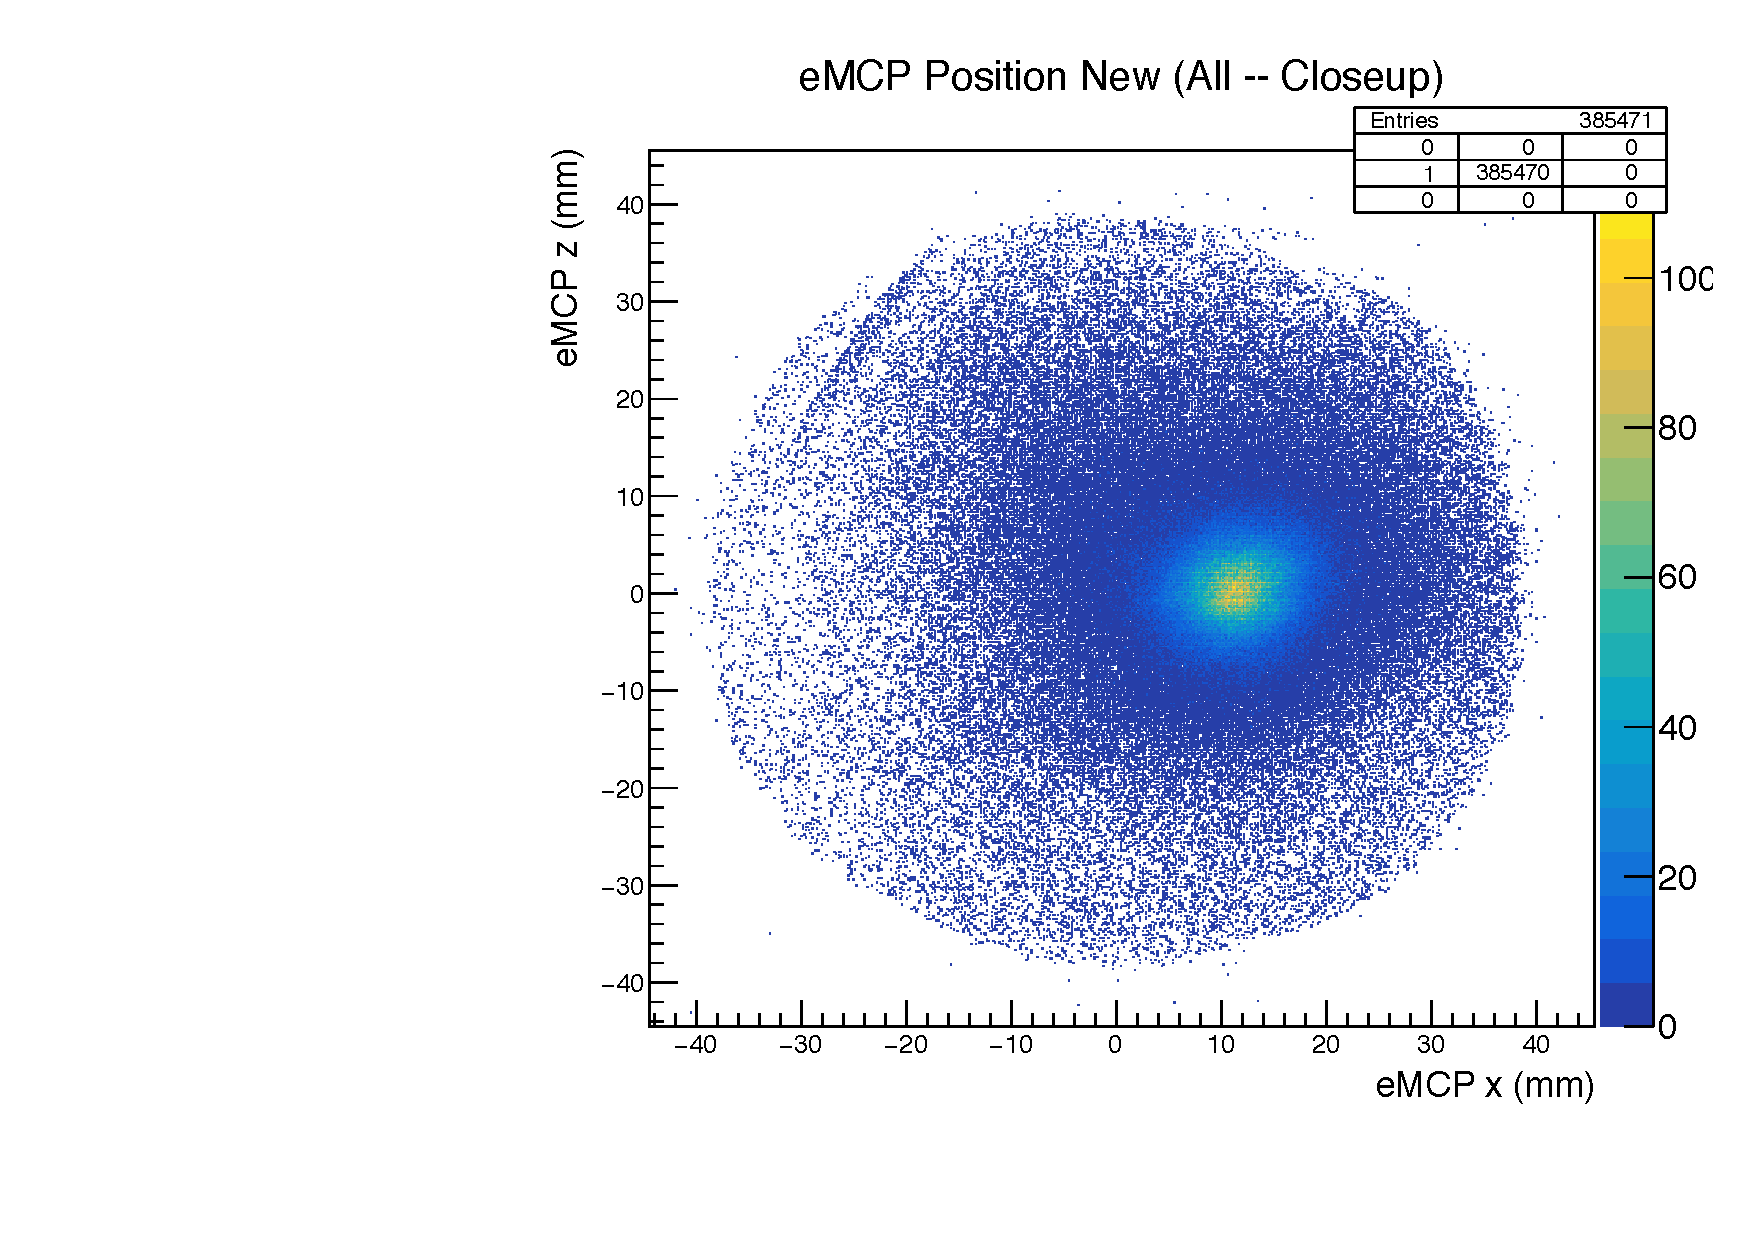
\includegraphics[width=.999\linewidth]
	{Figures/eMCP_position.pdf}
	\note{This picture is `slow'.  Need to re-save it as a png.}
	\caption{Position as measured on the eMCP, after some data cleaning.}	
	\label{fig:emcp_position}
\end{figure}

Because a SOE from the trap is most likely to land in the centre of the plate, while the background from other sources is roughly constant across the plate, it might make sense to accept only events where the eMCP hit is within some radius of the central peak.  This methodology was seriously considered because the remaining data has a much lower fraction of background events polluting it -- however this results in a loss of around half of the events even for the most generous eMCP radius cuts (see Fig.~\ref{fig:soe_tof_positioncompare}).  Therefore, it was decided that no position cuts on the eMCP would be made in the final analysis.

\begin{figure}[h!!!!t!]
	\centering
	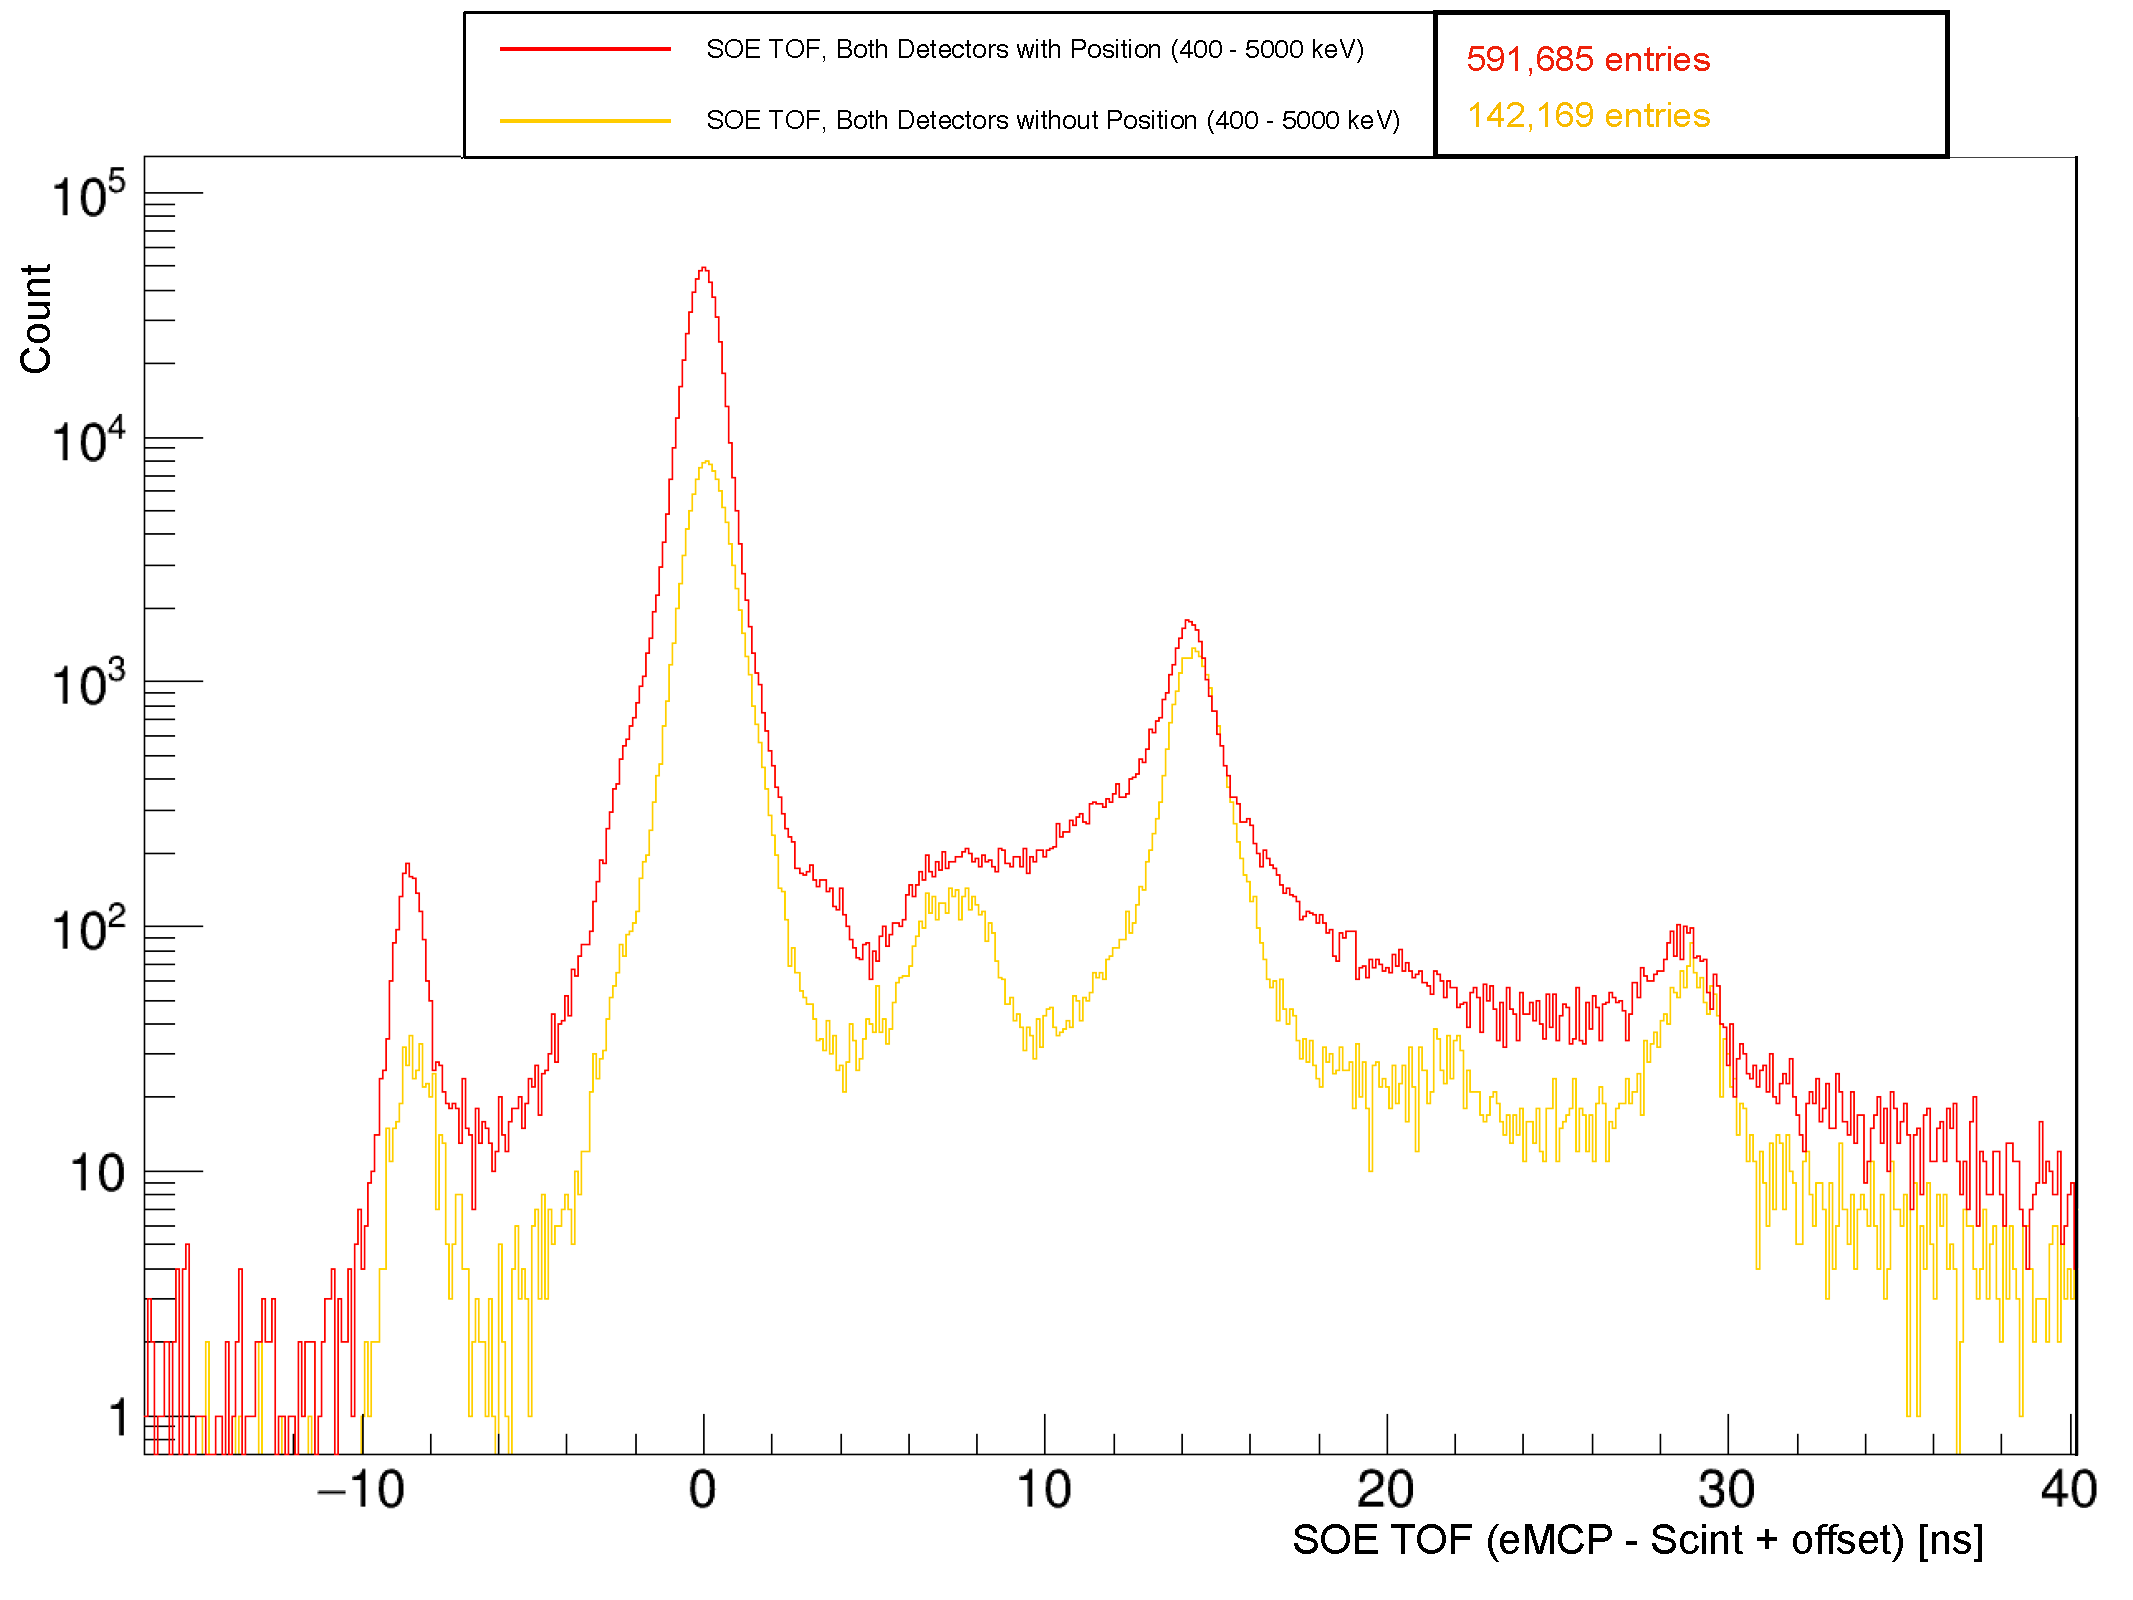
\includegraphics[width=.999\linewidth]
	{Figures/SOE_TOF_positioncompare.pdf}
	\note{Um.  Did I for sure get the labels correct on this???  It seems really wrong.}
	\caption{Beta-electron TOF, for events with and without eMCP hit position information.  A cut will eventually be taken to accept only events sufficiently near the largest peak -- in this case the number of events is `only' decreased by a factor of 2.}	
	\label{fig:soe_tof_positioncompare}
\end{figure}

Several years after the data was initially collected, a problem was discovered with our low-level analyzer software, which we had been using to convert large and unwieldy MIDAS data sets into somewhat smaller and more manageable ROOT data sets.  In particular, for every timestamp recorded, our raw MIDAS data actually included both a timestamp for the leading edge (LE) of the pulse, and a timestamp for the trailing edge (TE).  The analyzer had--for years--been reporting the timestamp associated with the trailing edge of the pulse.  Initially it was unclear if there might have been a reason behind this choice, but a closer examination of the data showed less timing noise and a sharper distribution of timing pulses across the board (see Fig.~\ref{fig:LE_TE}), with some channels showing a larger effect than others.  This was corrected, and the entirety of this analysis has been performed now using the cleaner LE spectra.  

\begin{figure}[h!!t!]
	\centering
	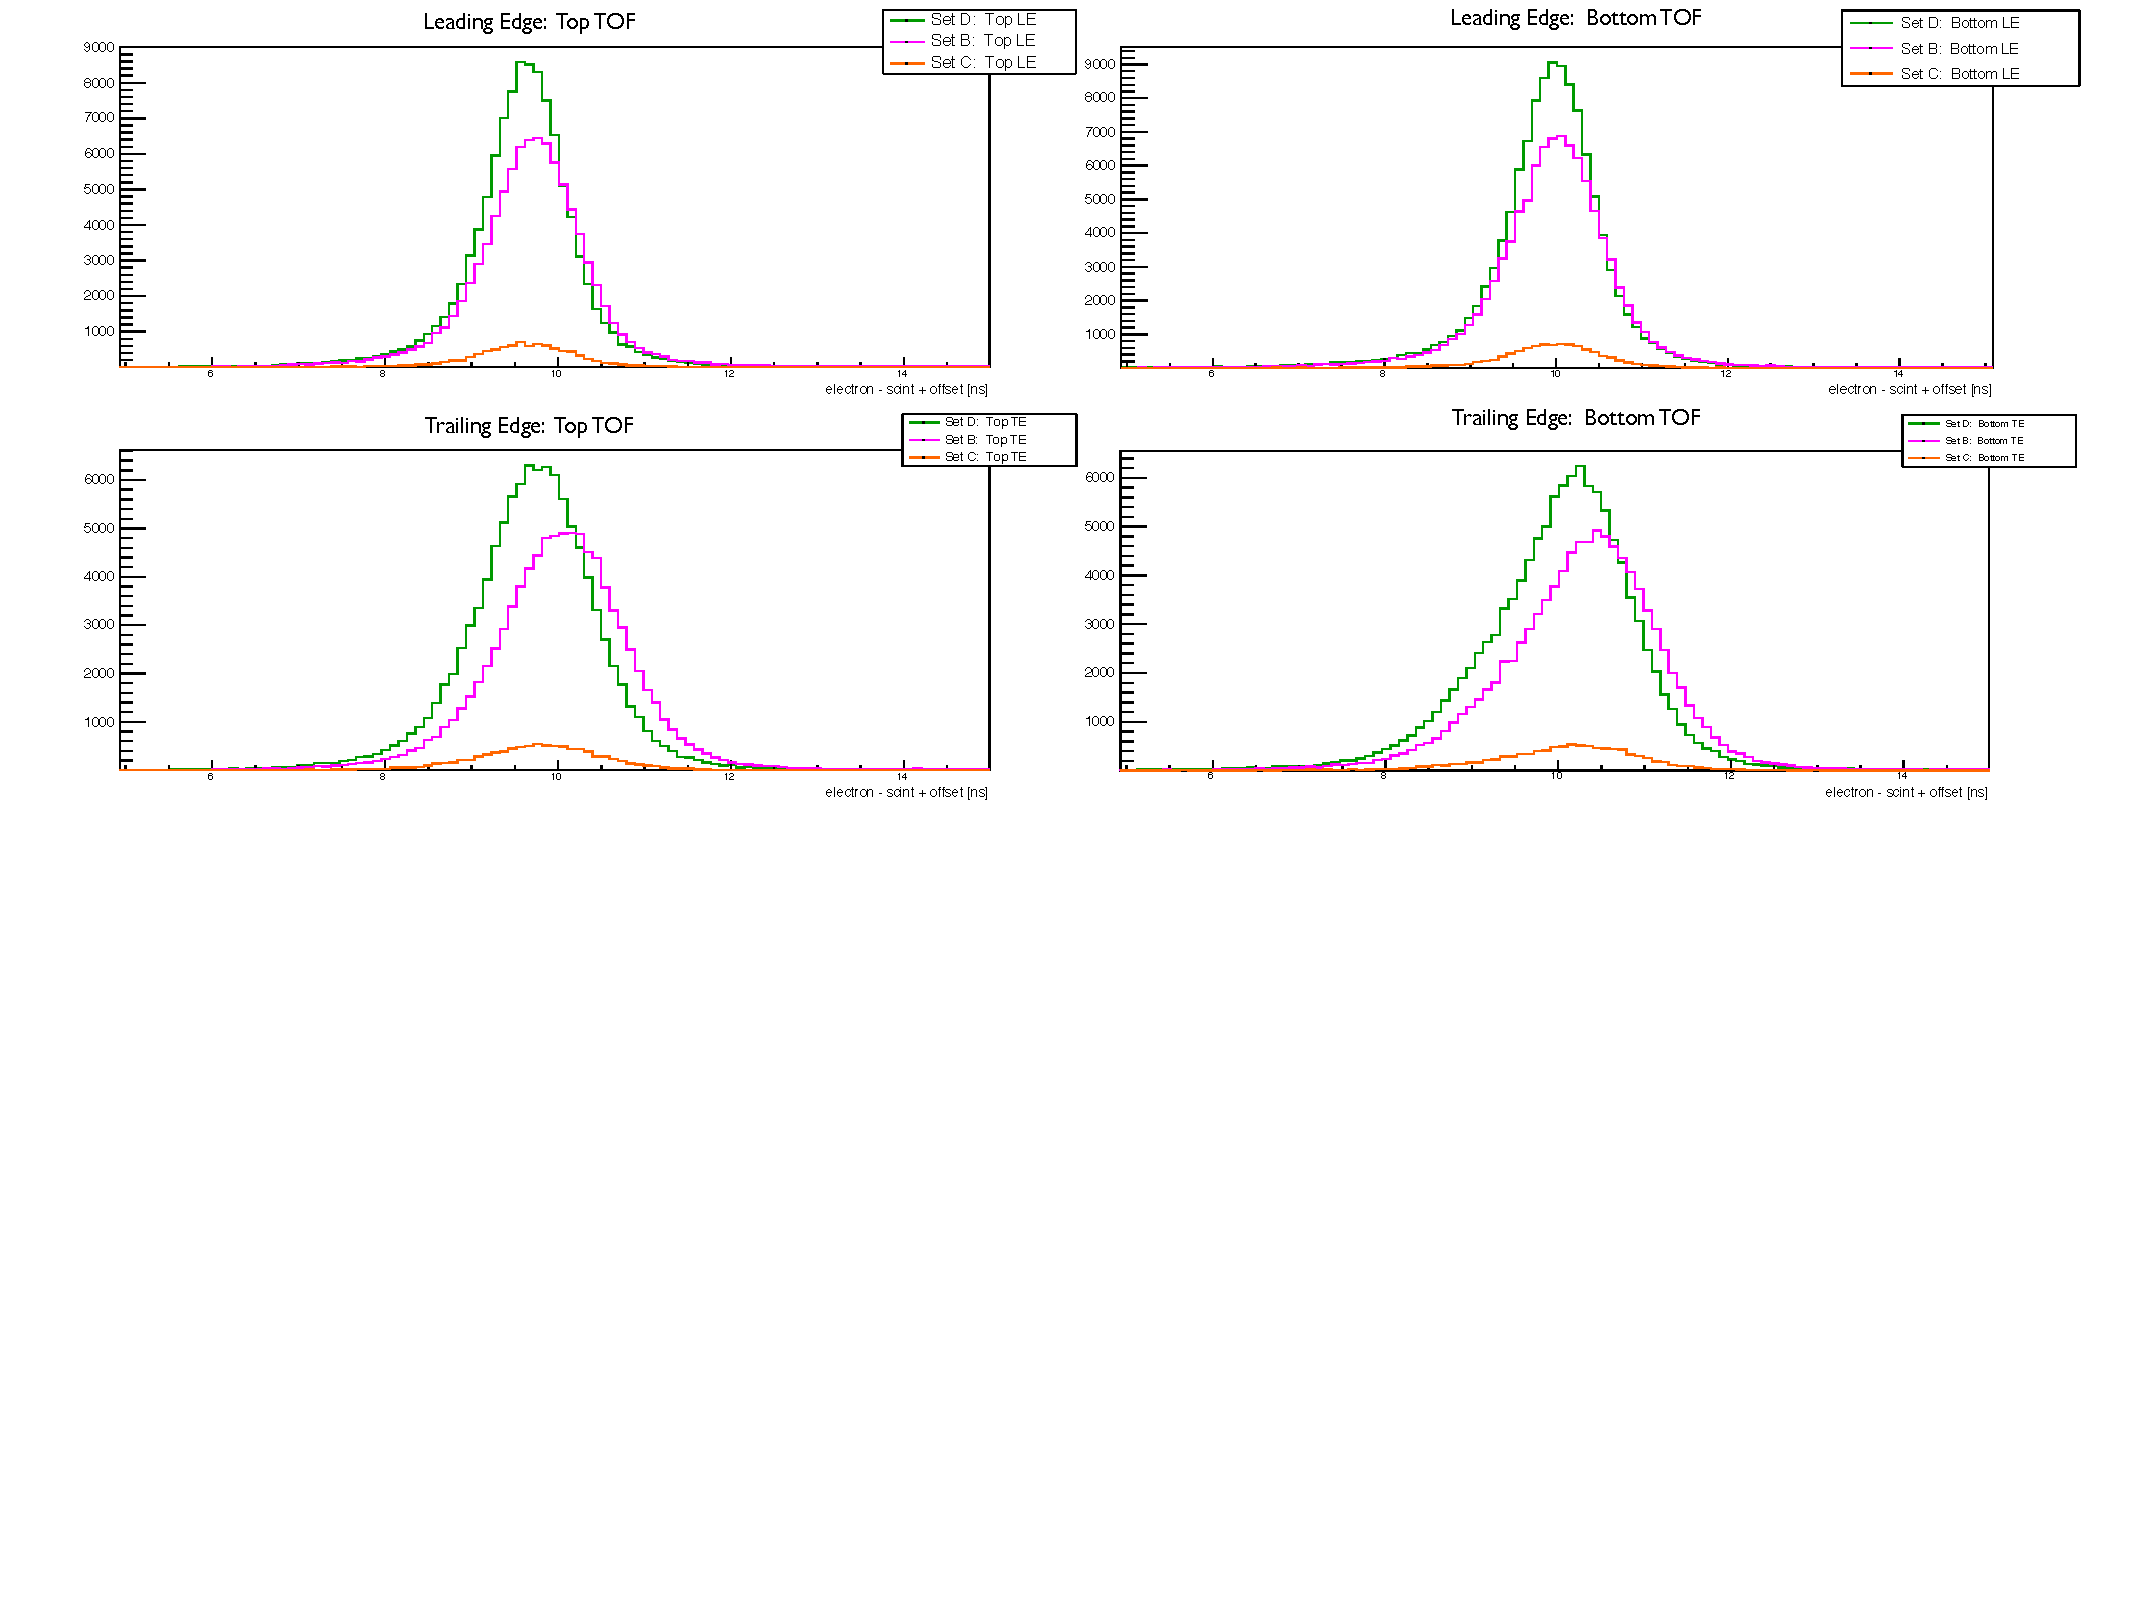
\includegraphics[width=.999\linewidth]
	{Figures/LE_TE_peaks.pdf}
	\caption{SOE TOF peaks (eMPC - Scintillator), using the leading edge (LE) and using the trailing edge (TE).  Data is sorted according to runset.  For each individual runset, the TE peak is broader than the LE peak.  The centroid of each runset is also more variable in the TE plots.}	
	\label{fig:LE_TE}
\end{figure}

The place where this change between the TE and LE timestamps had the biggest impact on the analysis is in the shake-off electron time-of-flight spectra, on which a cut must eventually be taken. Although this problem was not discovered in time to be used in the previous measurement of $\Abeta$ using this same data~\cite{ben_Abeta}, it likely would have had a negligible effect on the final result, because the SOE TOF cut that was used there was comparatively loose, and the evaluation of the background that remained was not a dominant systematic effect. \aside[color=org]{This goes in that one appendix, if I haven't already put it there.}

With the data reprocessed using the leading edge for timestamps, I wanted to eliminate as much background as possible from the SOE TOF spectrum.  With this goal in mind, the next step was to correct the scintillator timing for its low energy `walk' (see Fig.~\ref{fig:WalkAdjust}).  A quartic polynomial was fit to each of the 2D timing vs energy spectra (the top and bottom detectors were treated separately), and the result was used to produce a `straightened' SOE TOF spectrum with respect to measured scintillator energy, and as expected, the resulting SOE TOF spectrum was a bit more sharply peaked.  


\begin{figure}[h!!!!tb]
	\centering
	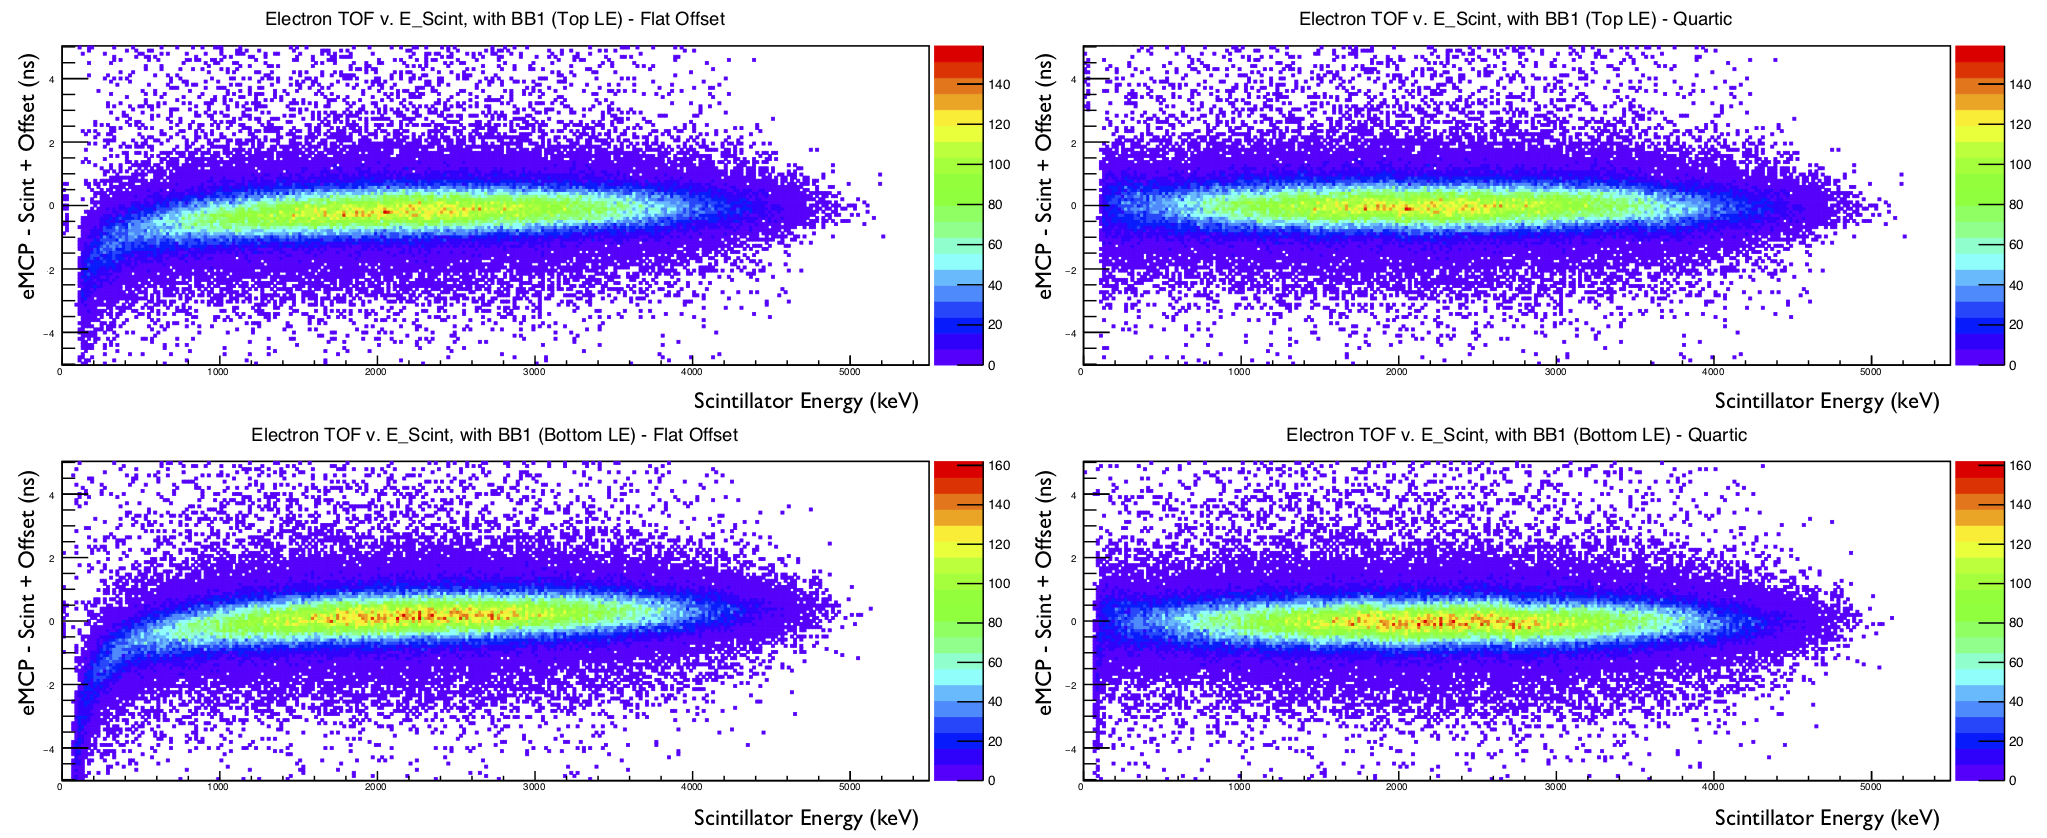
\includegraphics[width=.999\linewidth]
	{Figures/WalkAdjust.png}
	\caption{SOE TOF walk, before (left) and after (right) applying a quartic adjustment to straighten out the effective TOF.}	
	\label{fig:WalkAdjust}
\end{figure}

%At this point it becomes necessary to attempt to model the SOE TOF spectrum, as in Fig.~\ref{fig:soetof}.  
With the SOE TOF spectra cleaned up, a cut can be taken to reduce the fraction of background events.  Informed by the model of background spectra described in Section~\ref{sec:tof_bg}, a was made to include only a 2.344 ns window around the primary peak in further analysis \aside{``...removing X fraction of the remaining events."}. (see Fig.~\ref{fig:soetof}).
\note{Probably need to put that figure somewhere else.}

%For this analysis, the decision was made to use only events within a 2.344 ns window around the primary peak (Fig.~\ref{fig:soetof})  
%This part
%To understand the events that remain after this cut, it is necessary to create a model of the background events represented therein.   This is discussed in Section~\ref{sec:tof_bg}.

\note{``To check the agreement of the model with reality, we compare the averaged superratio asymmetries from both, as in Fig.~\ref{fig:asymmetry_by_tof}.'' .... probably goes in the other section.}
%\note{Okay.  This needs more description.}

\begin{figure}[h!!!!tb]
	\centering
	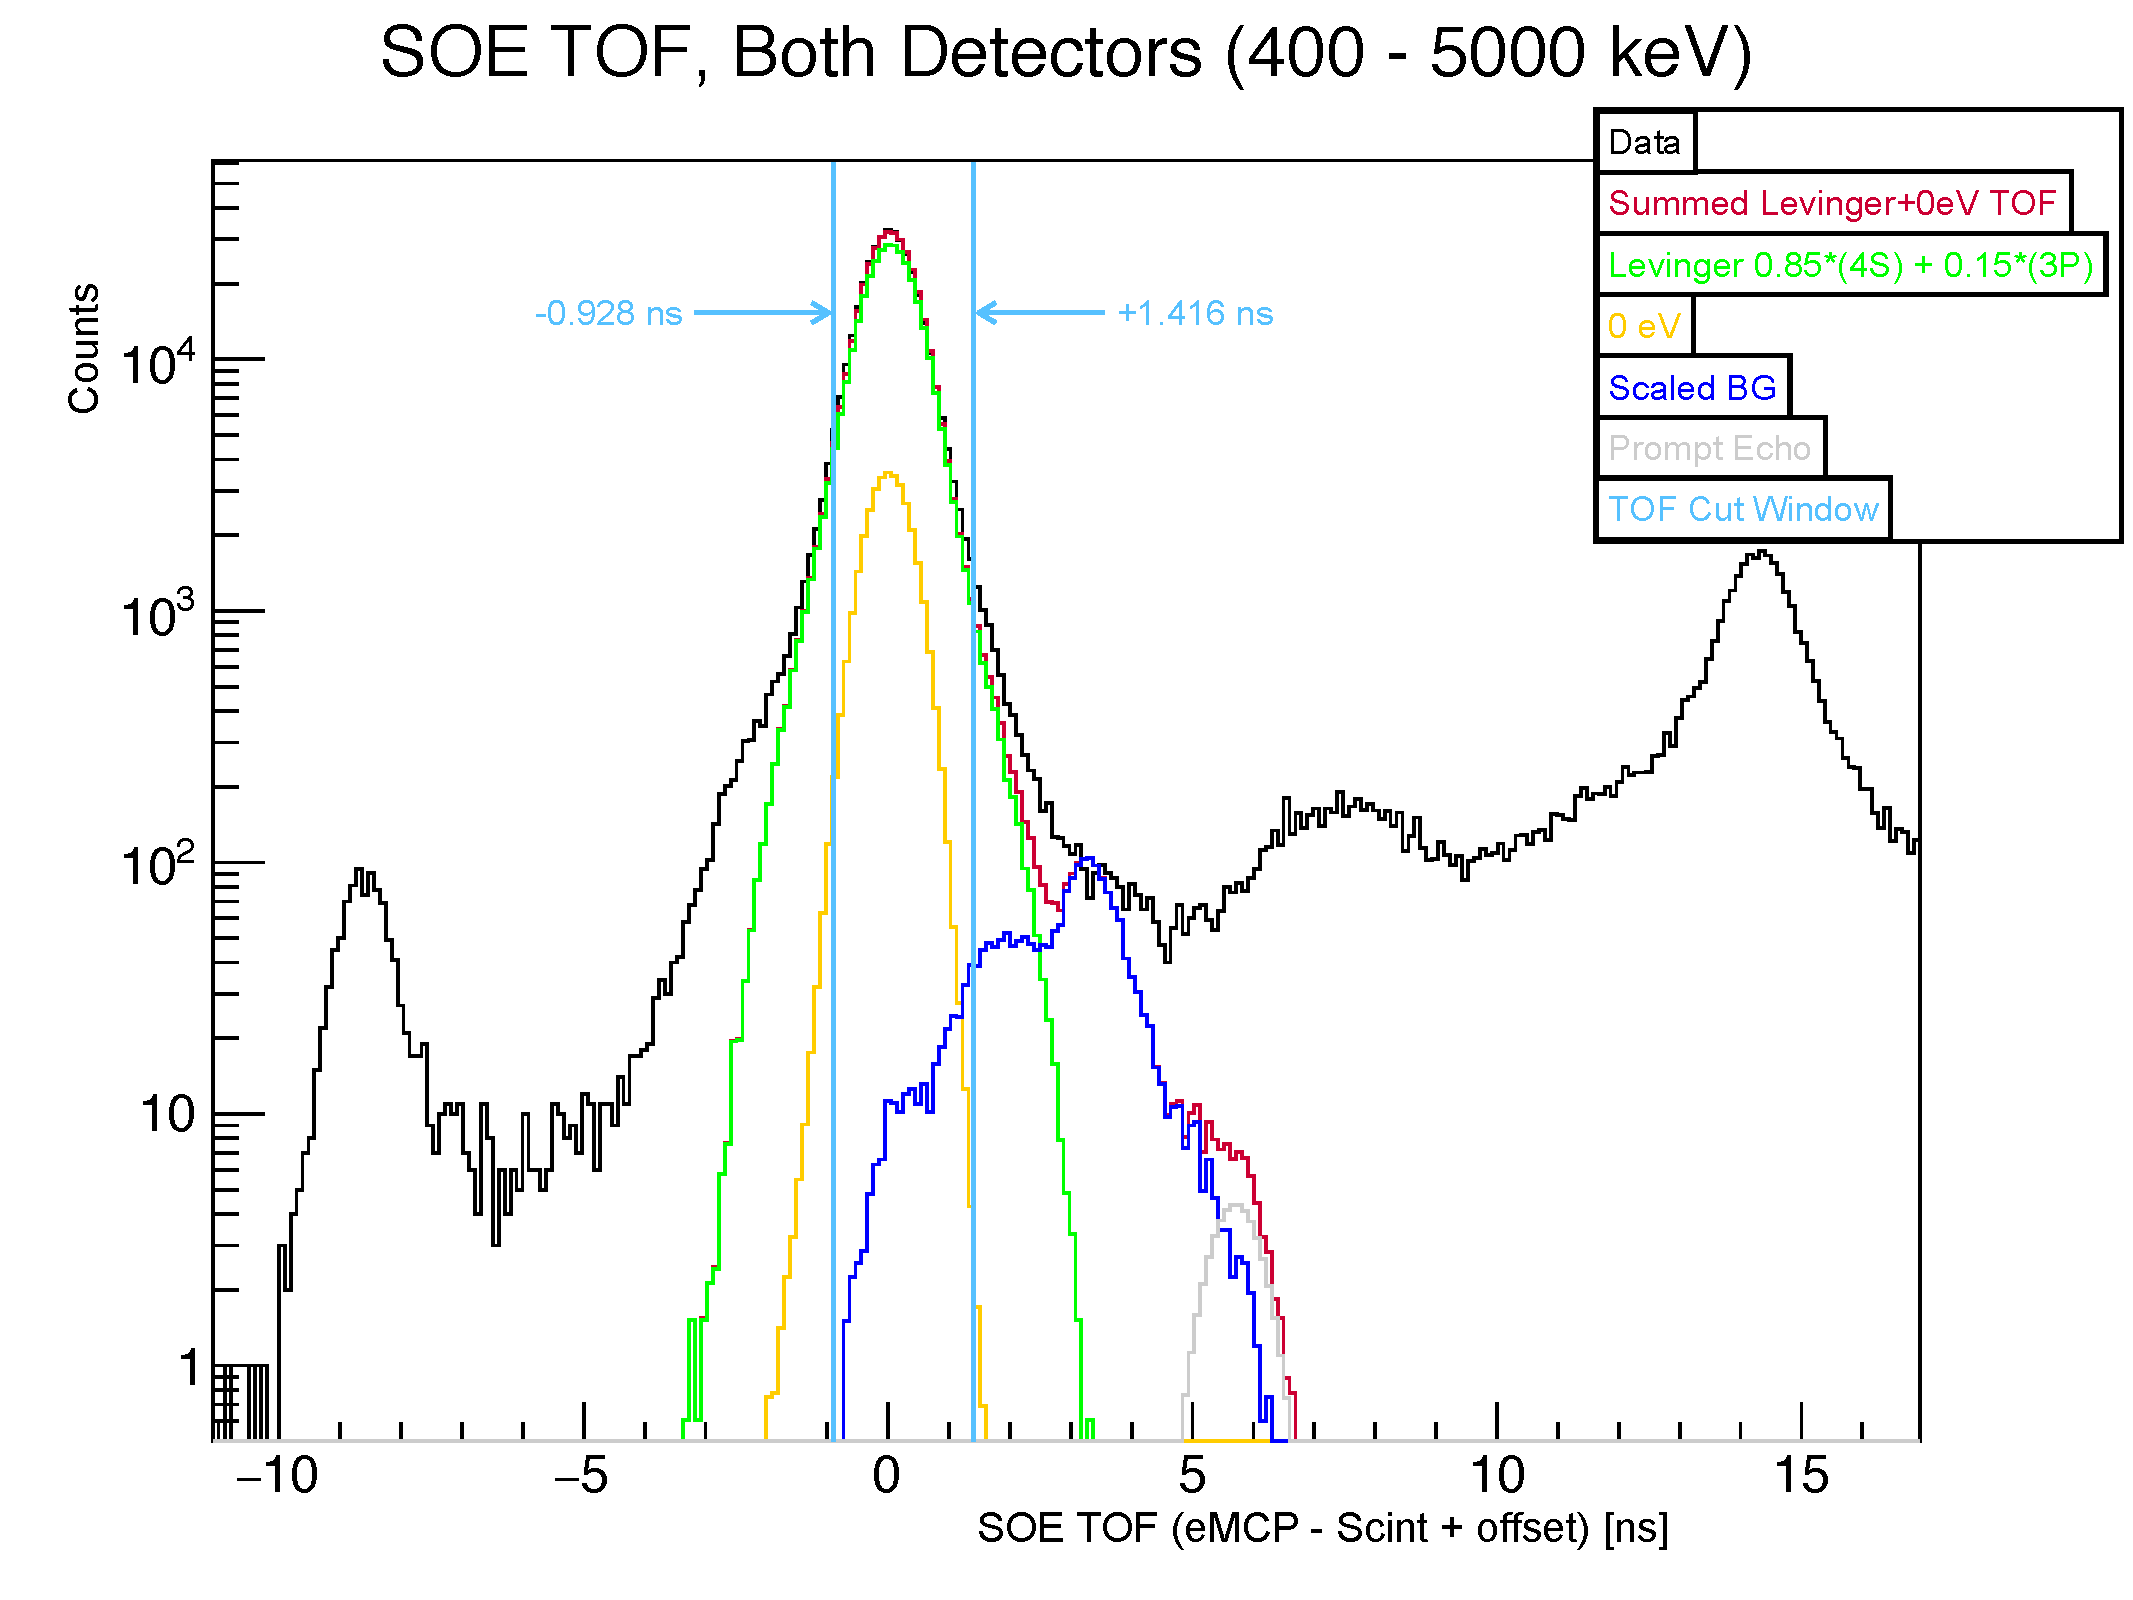
\includegraphics[width=.999\linewidth]
	{Figures/SOE_TOF_Spectra.pdf}
	\caption{SOE TOF, model and data.  In the end, I cut the data to use only events with a TOF between -0.928 ns and +1.416 ns.  Max. possible background is like a factor of two too big.  Similar quality results no matter how you distribute the Levinger spectra between 4S and 3P, however adding the 0 eV electrons makes a big improvement to the agreement. }	
	\label{fig:soetof}
\end{figure}

\begin{figure}[h!!!!tb]
	\centering
	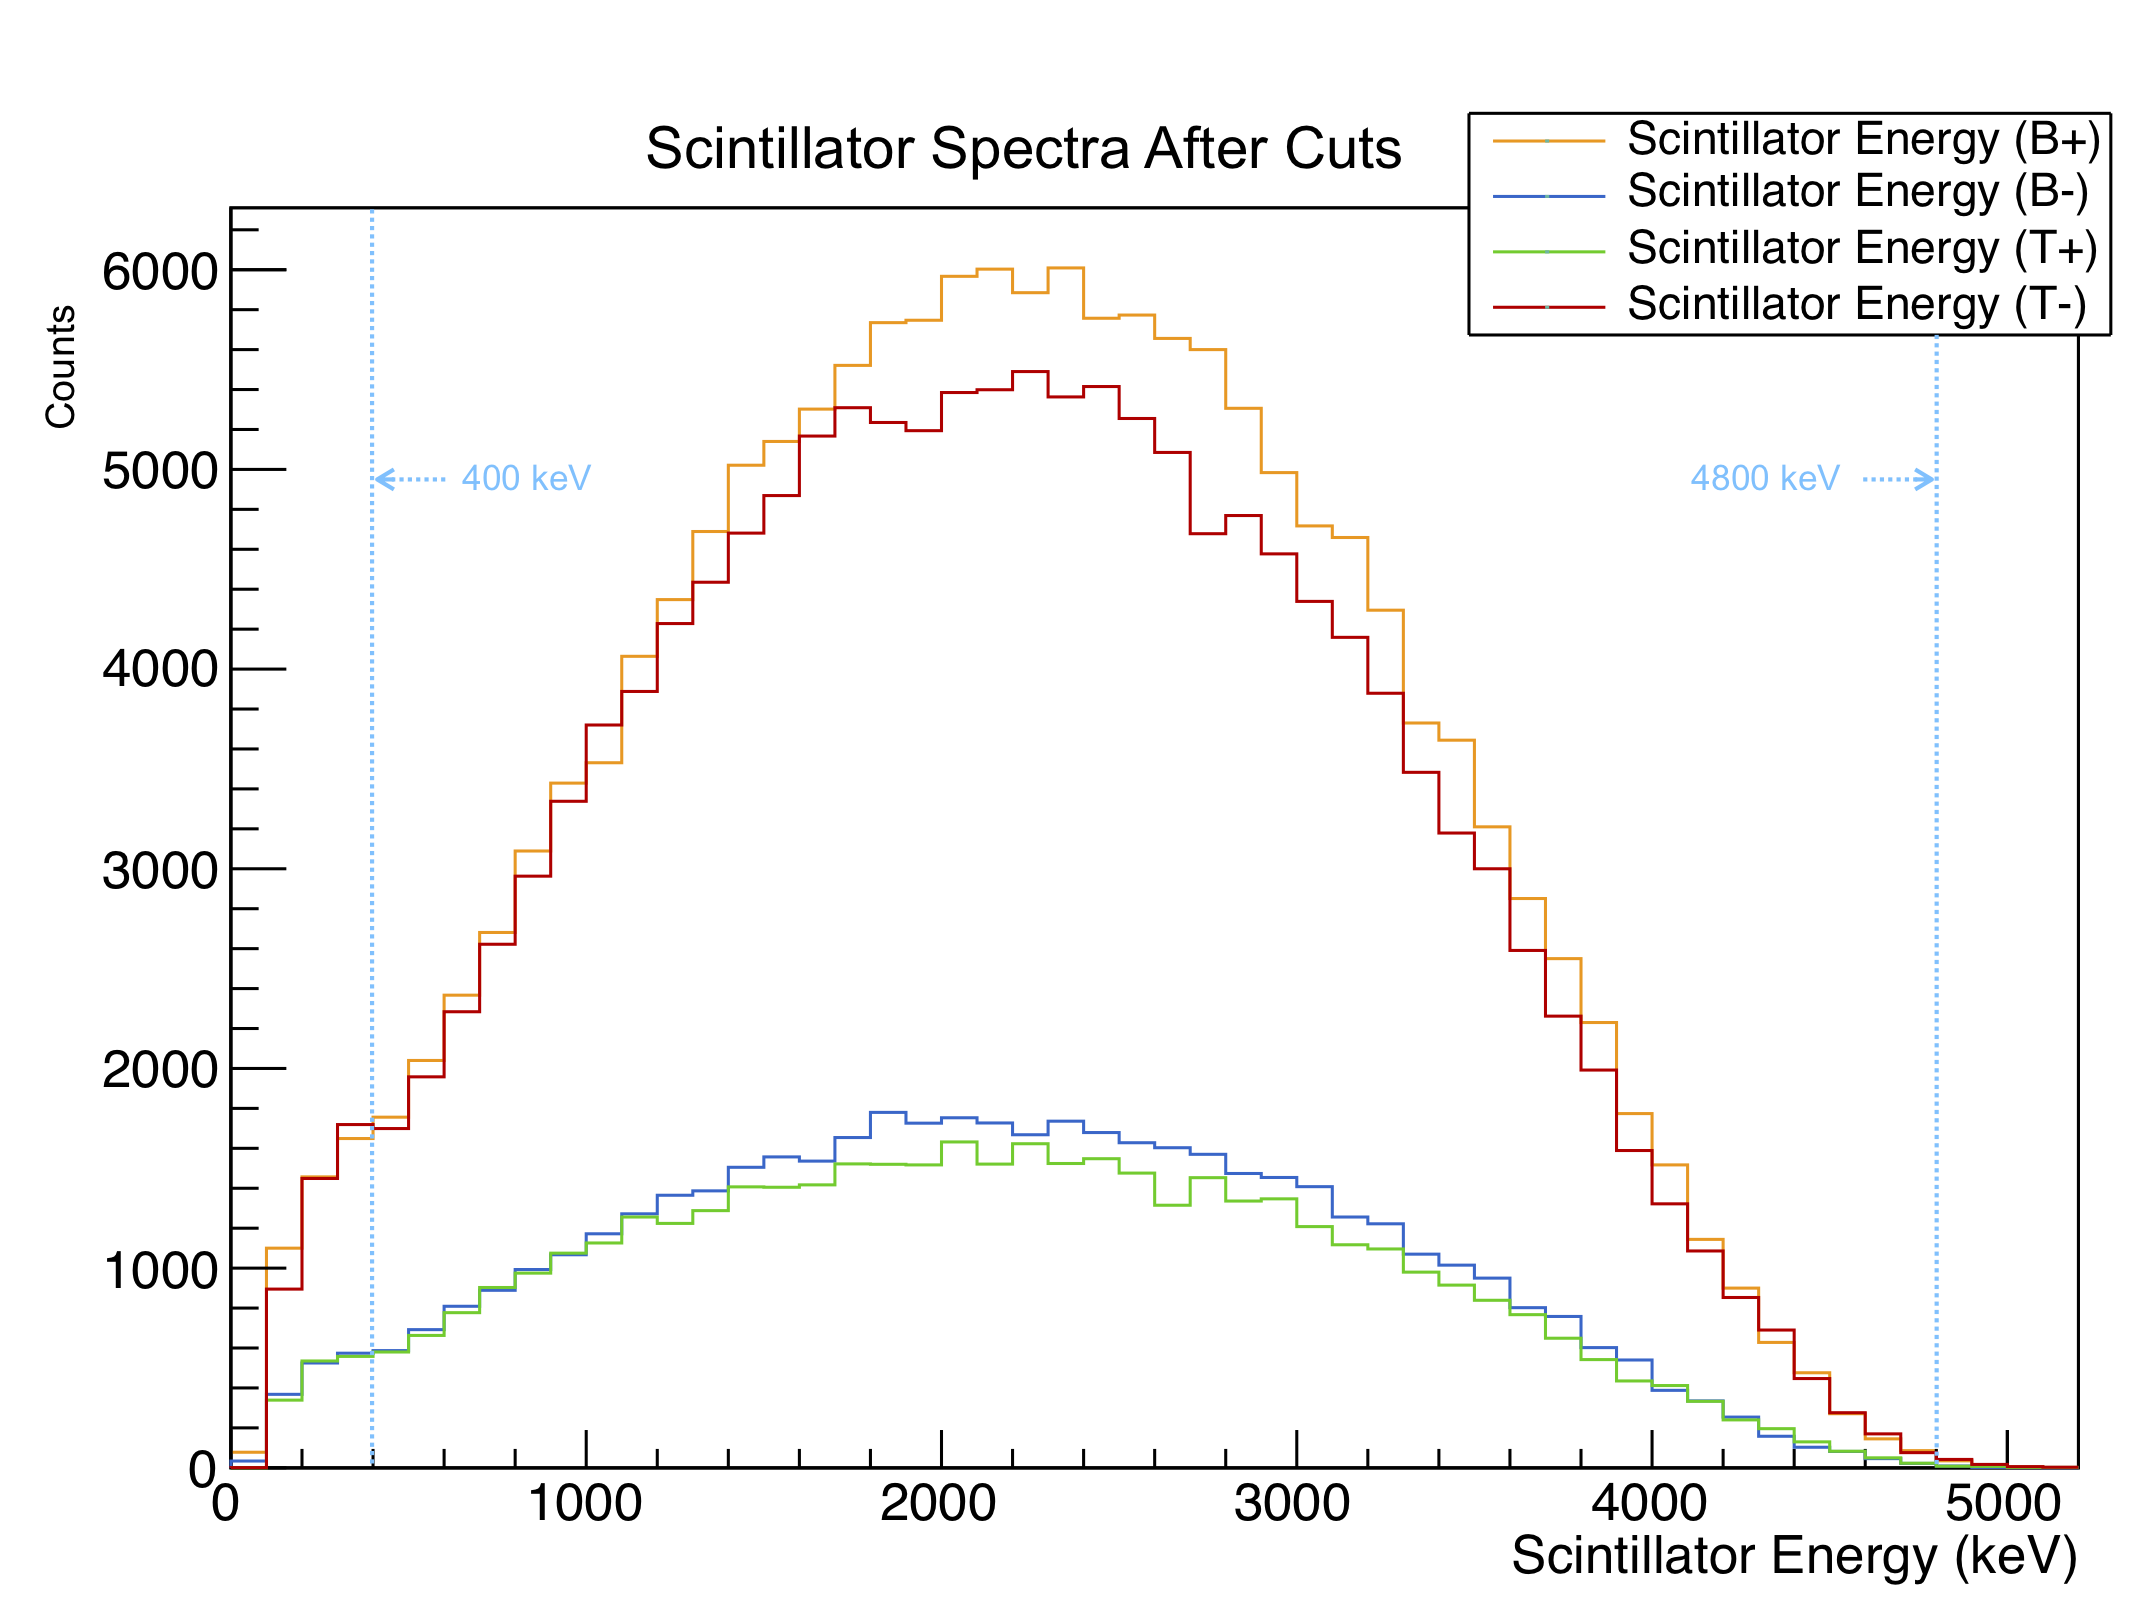
\includegraphics[width=.999\linewidth]
	{Figures/experimental_scintspectra_lin.png}
	\caption[Experimental Scintillator Spectra]{Experimental Scintillator Spectra, for both detectors in both polarization states.  These spectra are what remain after all cuts have been taken.  All runsets are included.}	
	\label{fig:scintspectra}
\end{figure}



\begin{figure}[h!!!!tb]
	\centering
	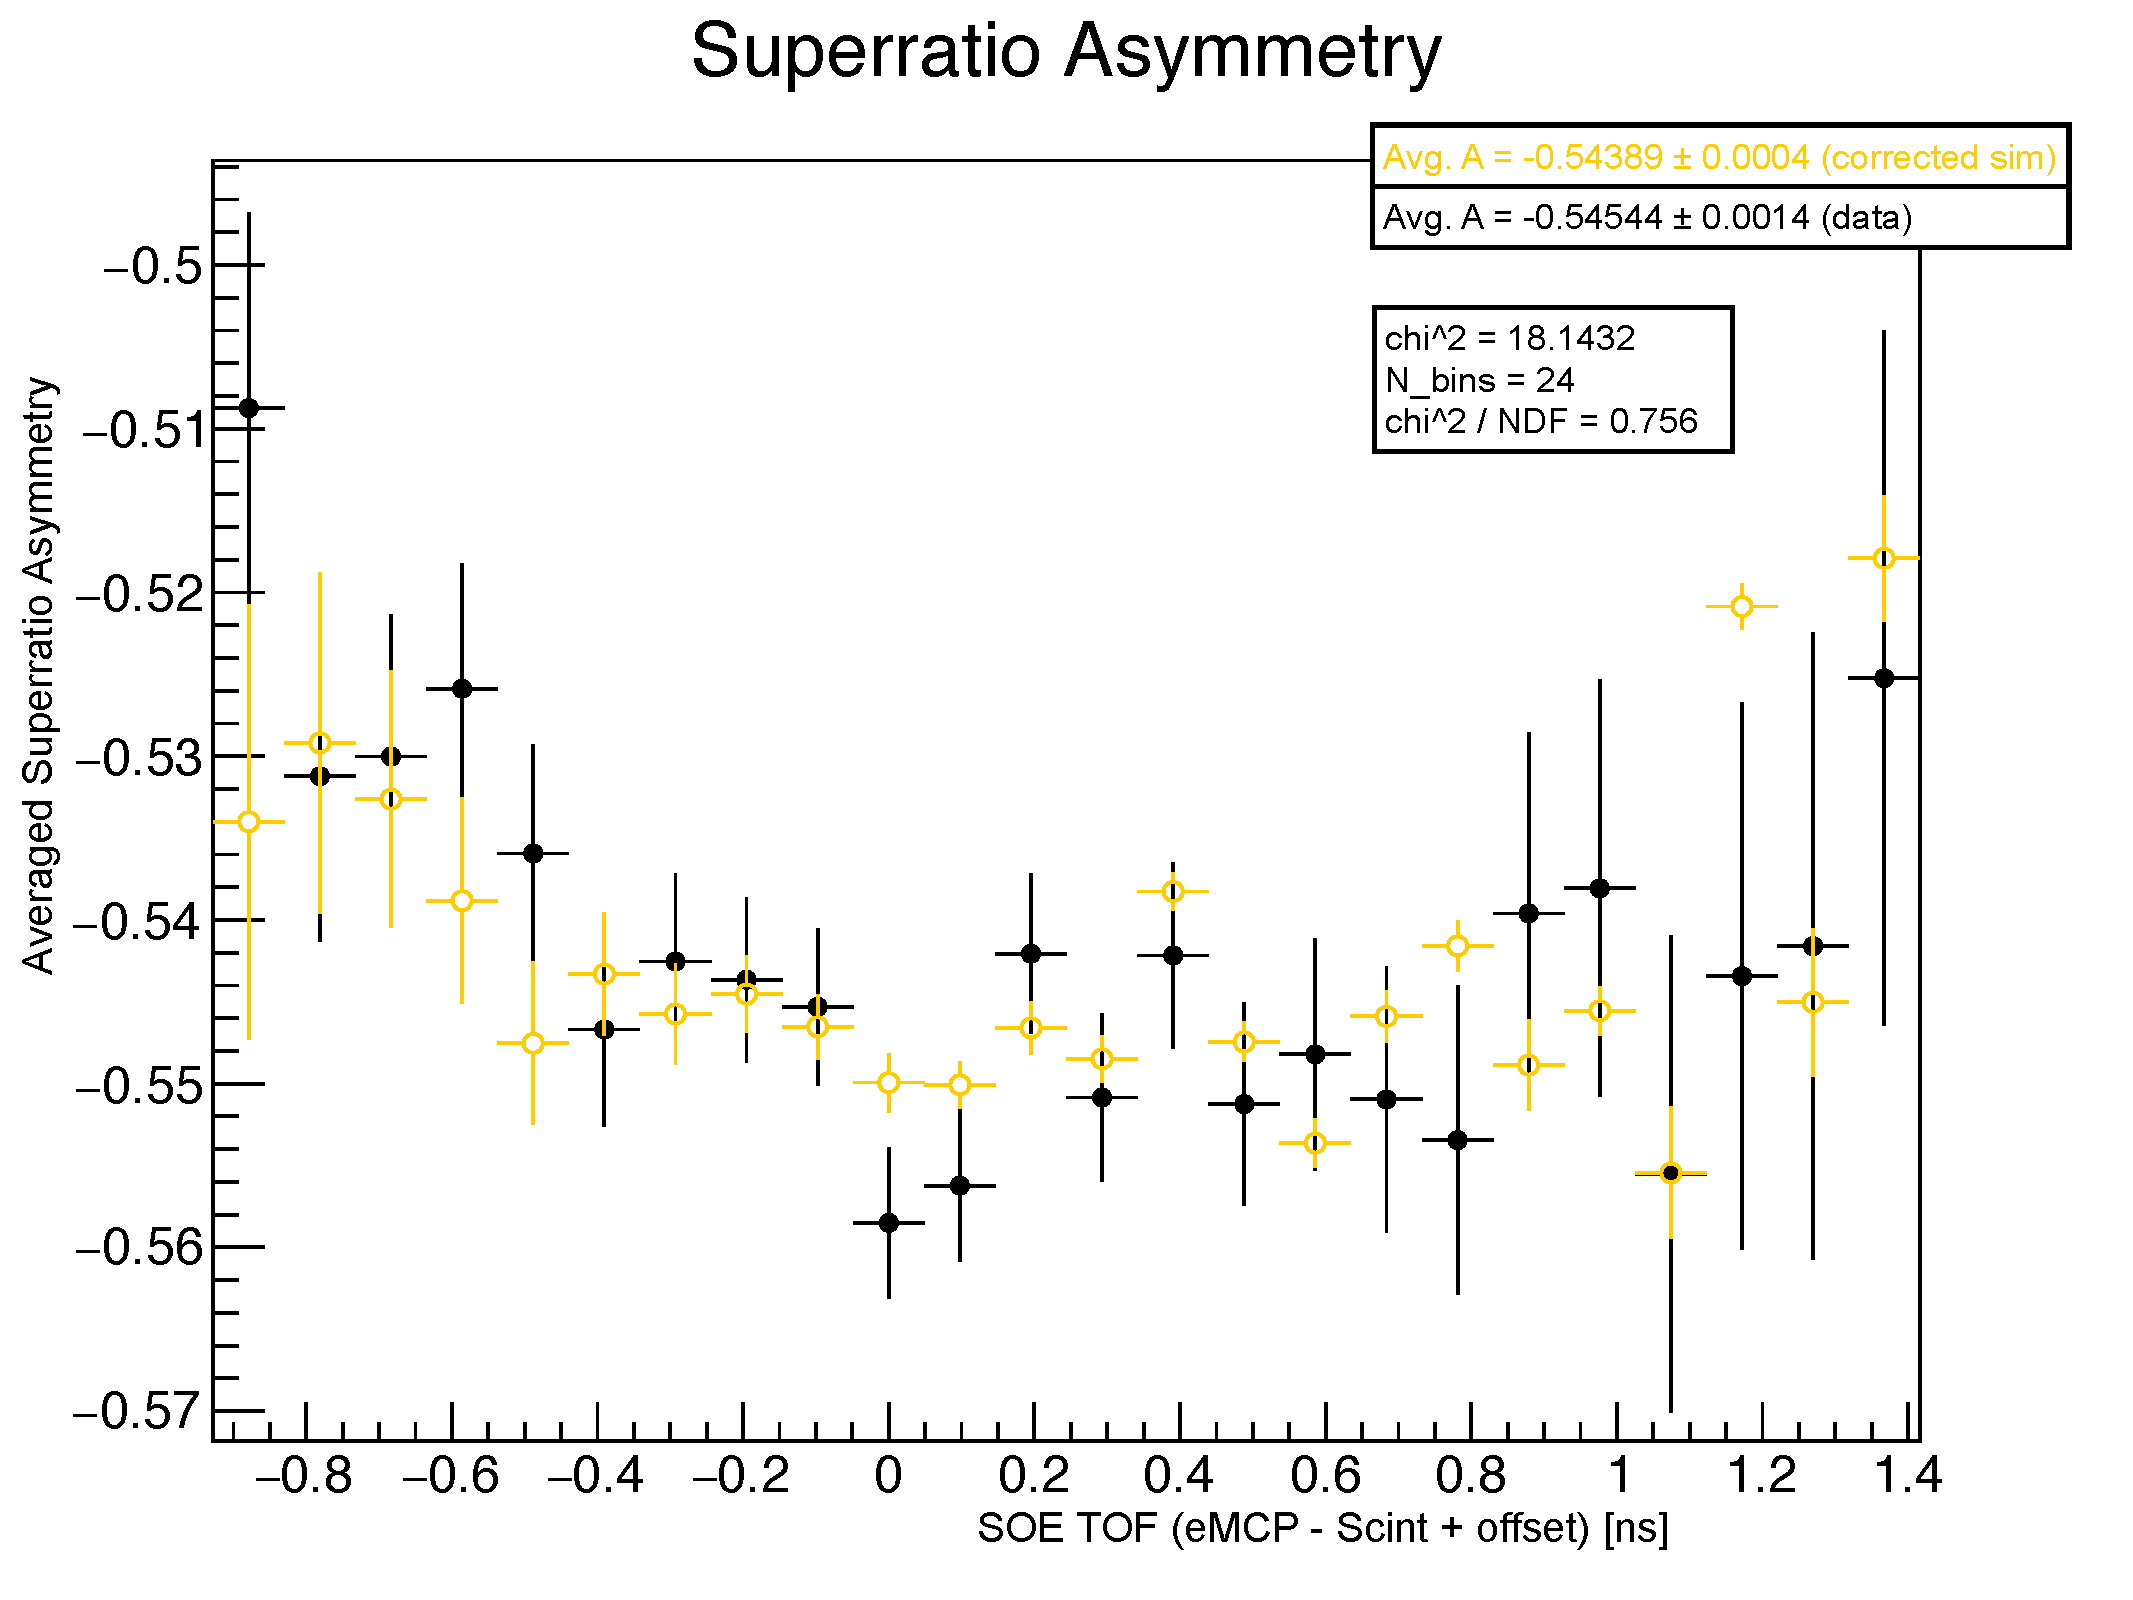
\includegraphics[width=.999\linewidth]
	{Figures/asymmetry_by_tof.pdf}
	\note{I think I want this picture to go in some other section.}
	\caption{The superratio asymmetry, averaged over all scintillator energies between 400-4800 keV, is used to compare the experimental data and simulated TOF model as a proxy for the quality of the model to estimate the background.  All other cuts have been applied.}	
	\label{fig:asymmetry_by_tof}
\end{figure}


%\section{Bullet Points!}
%Right, so.  Here's (more of) how I processed the data into an answer.  In bullet point form, so I don't forget stuff while I'm obsessively trying to phrase everything well.  
%\newline
%
%With the Data:
%\begin{itemize}
%%	\item \greycomment{Lower-level data cleaning.  Discard events during parts of the duty cycle when atoms weren't polarized.  Discard events near a recorded spark time. Discard events when the photoionization laser fires.  Discard events when the LED pulser used to calibrate the scintillators fires.}
%%	\item \greycomment{Split up runs into sets, to account for changing experimental conditions.  Possibly I should list what the differences between runs were somewhere.  But not in this section.  OTOH, ...maybe?}
%	%
%%	\item Make some more careful cuts to clean the data.  
%	%	\begin{itemize}
%%		\item \greycomment{Discard events without a ``good'' DSSD hit.  Eliminates vast majority of background 511s.  Necessitates having a definition of what a ``good'' DSSD hit is.  It's subtle enough that we'll want to leave some part of this definition of ``good'' to be varied as a systematic effect.  Notably, we consider energy agreement for each hit pixel, individual strip SNR, and overall DSSD energy threshold.  Also, hit radius w.r.t. center of detector.  This is a lot of stuff, all implemented by Ben -- and it needs to be done fairly early on in data processing in order to keep processing times for everything else manageable.  }
%		\item Discard events where SOE-Beta TOF falls outside a certain range.  Necessitates picking a ``good'' range.  The precise definition of ``good'' is varied as a systematic.  
%		\item \greycomment{There was a scintillator timing walk correction before taking the SOE-Beta TOF cut.}
%		\item \greycomment{Before the scintillator walk correction, there was the thing where the data was re-processed using the leading edge pulse rather than the trailing edge pulse.  Makes it cleaner.  Ben just got stuck with the trailing edge.}
%		\item \greycomment{Could have implemented an eMCP hit *position* requirement, but that kills too many stats.  It's like a factor of two.}
%	%	\end{itemize}
%\end{itemize}









%%%% --- * --- %%%%
% !TEX root = ../thesis_main.tex



%%%% --- * --- %%%%
\clearpage	
\chapter{Estimating Systematic Effects}
\label{systematics_chapter}

\note[color=jb]{JB:  ``I doubt I will have further useful comments on the Ch. 5, 8, 9 as they are now.
\\
I've tried to email you the paragraphs on "collaboration determination of uncertainties" for Ch. 9.
\\
My intent of all that other advice  was to keep your time spent on Chs 1-4 concise, so you could concentrate on these real jobs.  (n.b.:  the advice he's already sent was almost all about chapters 1-4, which are the various intros/background info and experimental setup stuff)
\\ ... \\
I can only say that if you have an equal choice between including a detail or not, pick "not." ''
}

\note[color=jb]{JB:  I will try to schedule meeting with Dan for you to show us the final version of Ch. 9 Estimating systematic effects soon.}

\note[color=org]{Do I want this chapter combined with the analysis chapter?  If that chapter includes all the stuff about G4, it's going to be unwieldy and huge.}
%\note{How do I even \emph{do} these estimations?}

\note[color=todoblue]{JB says:   
\\
A simple estimate from the collaboration that builds intuition for this result:
Scatter in the SiC mirrors and DSSD actually produces an efficiency change at low
beta energy. Energy loss is not minimally ionizing in these structures, and instead
will have a long Landau tail that can take events below energy threshold in the scintillator.
The collaboration has modelled explicitly the false asymmetry as a function
of Kbeta between 600 and 1300 keV, producing roughly (K-0.6 MeV)/(0.7 MeV), i.e.
50\% at Kbeta=0.95 MeV. This efficiency degradation would be distributed roughly equally
between the SiC and DSSD.
If completely ignored, this would introduce by inspection a false bFierz of approximately
0.5.
Scattering effects will vary between linear and sqrt of thickness, so assuming
worst case of linear, the mechanical thickness uncertainty
of 5 micron/300 micron and 6 micron /275 micron, an average of 2\%, making
a random contribution of order 0.01 each.
The Be window has larger mechanical thickness uncertainty of 23micron/229 micron, but
energy loss and scattering in this material is 5x smaller, so the net effect would be similar.
\\ ... \\
To minimize this systematic for future experiments, the collaboration has
implemented pellicle mirrors of negligible thickness, 100 nm Au on 4 micron
kapton. The collaboration is also implementing Be-windowed wire chambers in
place of the DSSD.
\\
...
\\
MJA:  .....huh?
}

\section{Overview}	
A summary of systematics goes here.  In words, yes, but also in table form.


% !TEX root = ../thesis_main.tex



%%%% --- * --- %%%%	
%\renewcommand{\arraystretch}{1.6}

\begin{table}[h!!!!t]
	\begin{center}
	\begin{tabular}{ l  c  c  }
		\multicolumn{1}{l}{ Source} 		& \multicolumn{2}{c}{ \;\;\; \;\;\; Uncertainty \;\;\; \;\;\; }   
		\\
		\multicolumn{1}{l}{ } 				& \multicolumn{1}{c}{\;\; $\bFierz$}   & \multicolumn{1}{c}{$\Abeta$}   	
		\\  \hline
		%%% % %%%
		Scintillator Calibration 			& 0.003								& 0.0003											
		\\
		Scintillator Threshold  			& 0.004 							& 0.0004 						
		\\
		%%% % %%%
		DSSD Individual Strip SNR 			& 0.006								& 0.0007													
		\\
		DSSD Energy Agreement	  			& 0.005 							& 0.0006 						
		\\
		DSSD Detection Radius	  			& 0.006 							& 0.0017 						
		\\
		DSSD Energy Threshold	  			& 0.005 							& 0.0005 						
		\\
		%%% % %%%
		Atomic Cloud			  			& 0.002 							& 0.0002 						
		\\
		%%% % %%%
		Background				  			& 0.004 							& 0.0003 						
		\\
		%%% % %%%
		Beta Scattering				  		& 0.031 							& 0.0025 						
		\\
		%%% % %%%
		Low Energy Tail				  		& 0.008 							& 0.0007 						
		\\
		%%% % %%%
		Mirror Thickness				  	& 0.013 							& 0.0017 						
		\\
		DSSD Thickness				 	 	& 0.013 							& 0.0017 						
		\\
		Beryllium Foil Thickness			& 0.004								& $\!\!\!\!\!\! < 0.0001$ 			
	%	\\
		%%% % %%%
		\\  \hline
		\multicolumn{1}{l}{ Total Systematics} & \multicolumn{1}{c}{0.039}  & \multicolumn{1}{c}{0.0041}
%		Total Systematics			  		& 0.056 							& 0.0055 						
		\\
		\multicolumn{1}{l}{ Statistics} 	   & \multicolumn{1}{c}{0.084}  & \multicolumn{1}{c}{0.0082}
%		Statistics				  			& 0.084 							& 0.0082 						
	%	\\  \hline
		%%% % %%%
	\end{tabular}
	\end{center}
	\caption[Error Budget]{Error budget for the two-parameter analysis for $\bFierz$ and $\Abeta$, with all data included.  All uncertainties are believed to be uncorrelated, and are added in quadrature.  Final results: 
	$\mbox{ $\bFierz = 0.033 \pm 0.084(\textrm{stat}) \pm 0.039(\textrm{sys})$ }$ and $\mbox{ $\Abeta = -0.5738 \pm 0.0082(\textrm{stat}) \pm 0.0041(\textrm{sys})$ }$. }
	\label{table:budget}
\end{table}

%\renewcommand{\arraystretch}{1}





%	\section{Low-energy Scintillator Threshold}
%	%\\*
	Choice of low-energy scintillator threshold has a large systematic effect...  \aside{It's actually not nearly as big as I'd originally expected.  It's huge in the lineshape thing, but pretty tiny in everything else.}


	\note[color=jb]{from John:  ``I used Ben's threshold when determining the uncertainty from the lineshape tail (UFTLT). 
If you're saying the UFTLT depends on the threshold used, ok, of course it does. But if you're claimiing that UFTLT depends on the **uncertainty** of the threshold, that's manifestly smaller than the UFTLT itself, and I'm going to assert it isn't worth evaluating.''}
	
	\section{BB1 Radius, Energy Threshold, Agreement}
	\label{section:bb1_systematics}
	%\\*
	BB1 radius cut can help to eliminate scattered events.  Energy threshold selection and statistical agreement between BB1 detectors' energies only makes a small effect on results.  BB1 radius itself has a pretty big effect on the result, but we can at least just G4 it away.  The remaining systematic effect is pretty small.  
	\note[color=jb]{JB:  I hope the discussion is clear in your head.  Any effect that relies on scattering computation in G4 should have an uncertainty on order 10\% of the correction -- hopefully you are keeping a distinction here between the finite geometry acceptance (which I guess is exact) scattering off the collimator.}
	\note[color=jb]{As per JB's comment in section~\ref{thesisconventionjb}:   ``statistical agreement between BB1 X and Y detectors' energies only makes a small effect on results" does not need the technical details beyond that statement."}
	
\missingfigure{Surely this requires at *least* one image of the pixelated BB1 data.  Maybe some of a few waveforms and energy distributions too.  ....Feels like cheating to include some of that stuff, since Ben was the one who actually used it mostly.}
\note[color=jb]{JB on missing figure:  ``if you used such an image as part of your uncertainty estimate, yes [include it]''}

\note{Remember:  There's noise applied to simulated BB1s, matching some spectrum.}
In the end, we get our results from the scintillator energy only, without summing the BB1 energy back in.  Energy absorbed in DSSDs is only used as (a) a tag for events, and (b) contributing to the total beta energy loss before the beta arrives at the scintillator.
\note[color=jb]{JB:  The simulations of course include it event-by-event, not just a minimally ionizing average loss.}

\section{Background Modeling -- Decay from Surfaces within the Chamber}
	So many surfaces, all of which can get stray 37K atoms stuck to them.  Then they decay from a place that isn't the actual trap center, and it contaminates our stuff.
	
%	\missingfigure{Show modelled TOF spectra in comparison with real TOF spectra.  Show the cut we made on that. }
	\note[color=jb]{JB on figures that might go here:  Figure 6.4 (currently that picture of the TOF spectrum) could either be here, or you could reference it from here. The TOF histogram is a great start. Adding the asymmetry[TOF] indeed would be vital.}
	\missingfigure{Show the "average asymmetry" (all energies) as a function of TOF, with real data, best model normalization, and extrema of model normalizations.  Show our cut.  Turns out, it's a lot of work for a really tiny correction.  Oh well.}
	\note[color=jb]{JB on the *actual* figure I had been planning to put here, and my remarks about it:  Indeed it will be critical to show a clear compelling version of this figure in thesis and in a paper.  It was vital to minimize and determine this background to avoid fitting a polynomial to it from the wings,  even more so for the energy dependence of A than for its average -- you should say so.
	\\ ... \\
The reason the correction is small is because of all your hard work.}
	
	We model the beta TOF from the surfaces in G4, event by event.  This is necessary because scattered \aside[color=jb]{JB:  ``I wouldn't call these "scattered" events... that's very misleading.'' 
	\\ ... \\ 
	Yeah, I should really stop doing that.  
	\\ ... \\ 
	Wait no, scattered is what I mean!  But fine, my phrasing is really unclear.} events will have their TOF changed to account for a longer beta pathlength, and we're preferrentially cutting away the events that don't have a TOF in the appropriate range.  ....And then have COMSOL generate electron TOFs for SOEs starting from the start points picked by G4.  Ran COMSOL for 0 eV SOEs, and again for Levinger spectrum SOEs.  Used ~9\% 0eV SOEs in the end.  I forget which Levinger distribution I used in the end.  \aside[color=jb]{JB:  Please comment on whether or not it was important to have this energy distribution.}  The point is, for each event, you've simulated a beta TOF that may or may not be scattered off of something before it hits a detector, and you have a SOE TOF for an event originating at that same point, so you subtract them to model the TOF you'd measure in an experiment.  Also, because you've done the scattering with G4, you get the beta energy corrected for any scattering that happened.  This way, one can estimate %\aside[color=jb]{JB:  `you know precisely' $\rightarrow$ `you can estimate'} 
how many ``bad" events are eliminated with the TOF cut, as well as the fraction of ``bad'' events left in what remains.
	
%	\subsection{Decay from Chamber Surfaces}

\section{Quantifying the Effects Backscatter with Geant4}
	Beta decay (back-)scatter from surfaces within the experimental chamber is a significant systematic, and it must be evaluated, quantified, and corrected for.  This is done via a series of GEANT4 simulations.  While only a small fraction of events are affected, the process results in an energy loss in the beta that can, if not understood, be misinterpreted as the exact signal we're searching for.  It is therefore imperative that this be well understood. 
	
%	\aside{Oh god.  Have I even \emph{tried} to quantify the combined systematic that comes out of the TOF cut?  Do I need to, or is it double-counting?  Ugh, it would be such a headache to do this.  Maybe I can at least do it at the end -- because I might never get my code back to the way it was.}

\note[color=jb]{JB says: I would say you have a well-determined TOF cut to minimize this error-- a cut that could not have been done blind without an unreasonably perfect simulation.  Thus the exact spot of the cut should not be considered to introduce a systematic. }


%	\missingfigure{Show simulated $\cos\theta$ vs TOF.  You can just make a lot of that go away with a properly selected cut.}
\begin{figure}[h!!!t]
	\centering
	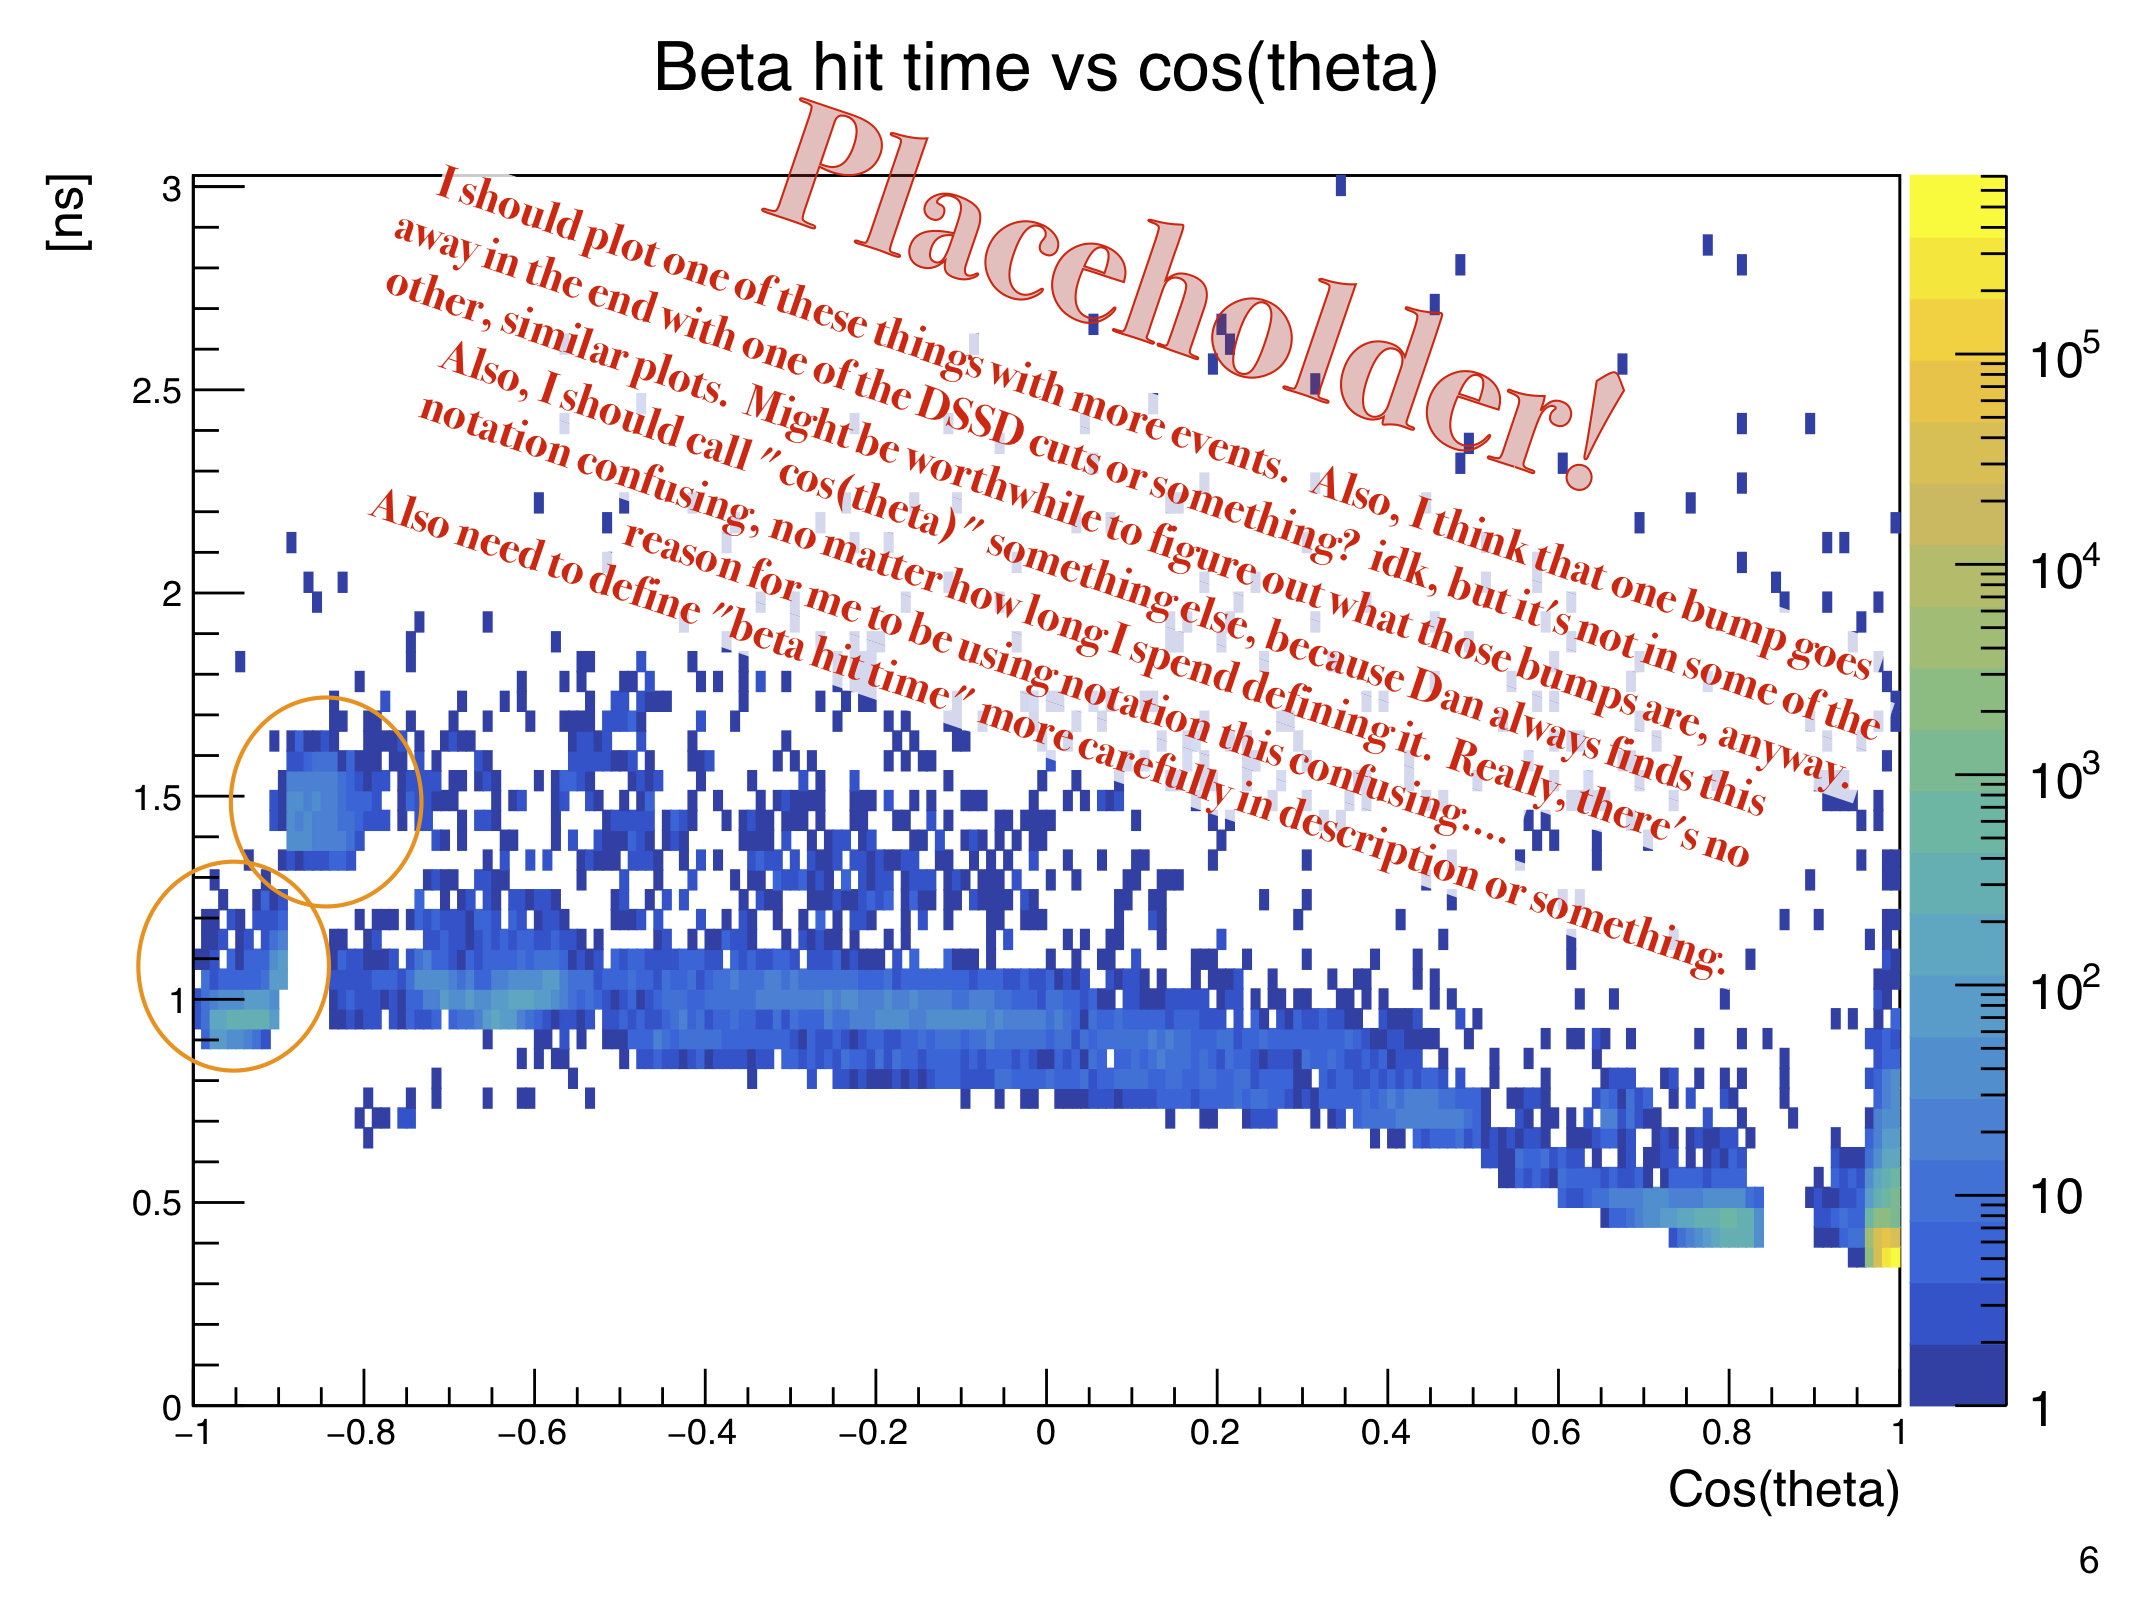
\includegraphics[width=.999\linewidth]
	{Figures/toa_vs_costheta.png}
	\caption[Simulated Beta TOA vs emission angle w.r.t. detector orientation]{Simulated Beta TOA vs emission angle w.r.t. detector orientation}	
	\label{fig:toa_vs_costheta}
\end{figure}

%\note[color=jb]{JB says:  
%Please discuss this at the next meeting.  (ETA:  Done!)
%\\
%Indeed this is why you should avoid calling the events originating not from the trap 'scattered events.' More importantly, why it was so critical that you reduced the size of the correction by timing bad events out. I would say you have a well-determined TOF cut to minimize this error-- a cut that could not have been done blind without an unreasonably perfect simulation.  Thus the exact spot of the cut should not be considered to introduce a systematic. }

%%%% --- * --- %%%%
\section{Lineshape Reconstruction}
	\note[color=jb]{This section should reference Clifford.~\cite{clifford}.}
	\subsection{Motivation}
	This process is used because the (back-)scatter, which it itself an important systematic, is largely independent of a wide variety of other experimental effects.  These other effects must all be evaluated, but it is computationally prohibitive to re-evaluate the scattering with every other effect under consideration.
	
	\subsection{What is it and how does it work?}
	Mono-energetic beta decay events are generated in GEANT4, which outputs an energy spectrum for unscattered and forward-scattered beta events in the detector.  These spectra are fit to a function to model the scintillator resolution, as well as energy loss in materials that the beta passed through before arriving at the scintillator.  These spectrum fits are performed for a set of beta energies, and parameters are extrapolated to be applied to betas emitted at intermediate energies.  Thus, the whole spectrum can be modeled.  Pictures will make this clearer. 
	
    \begin{figure}[h!!!t]
    	\centering
    	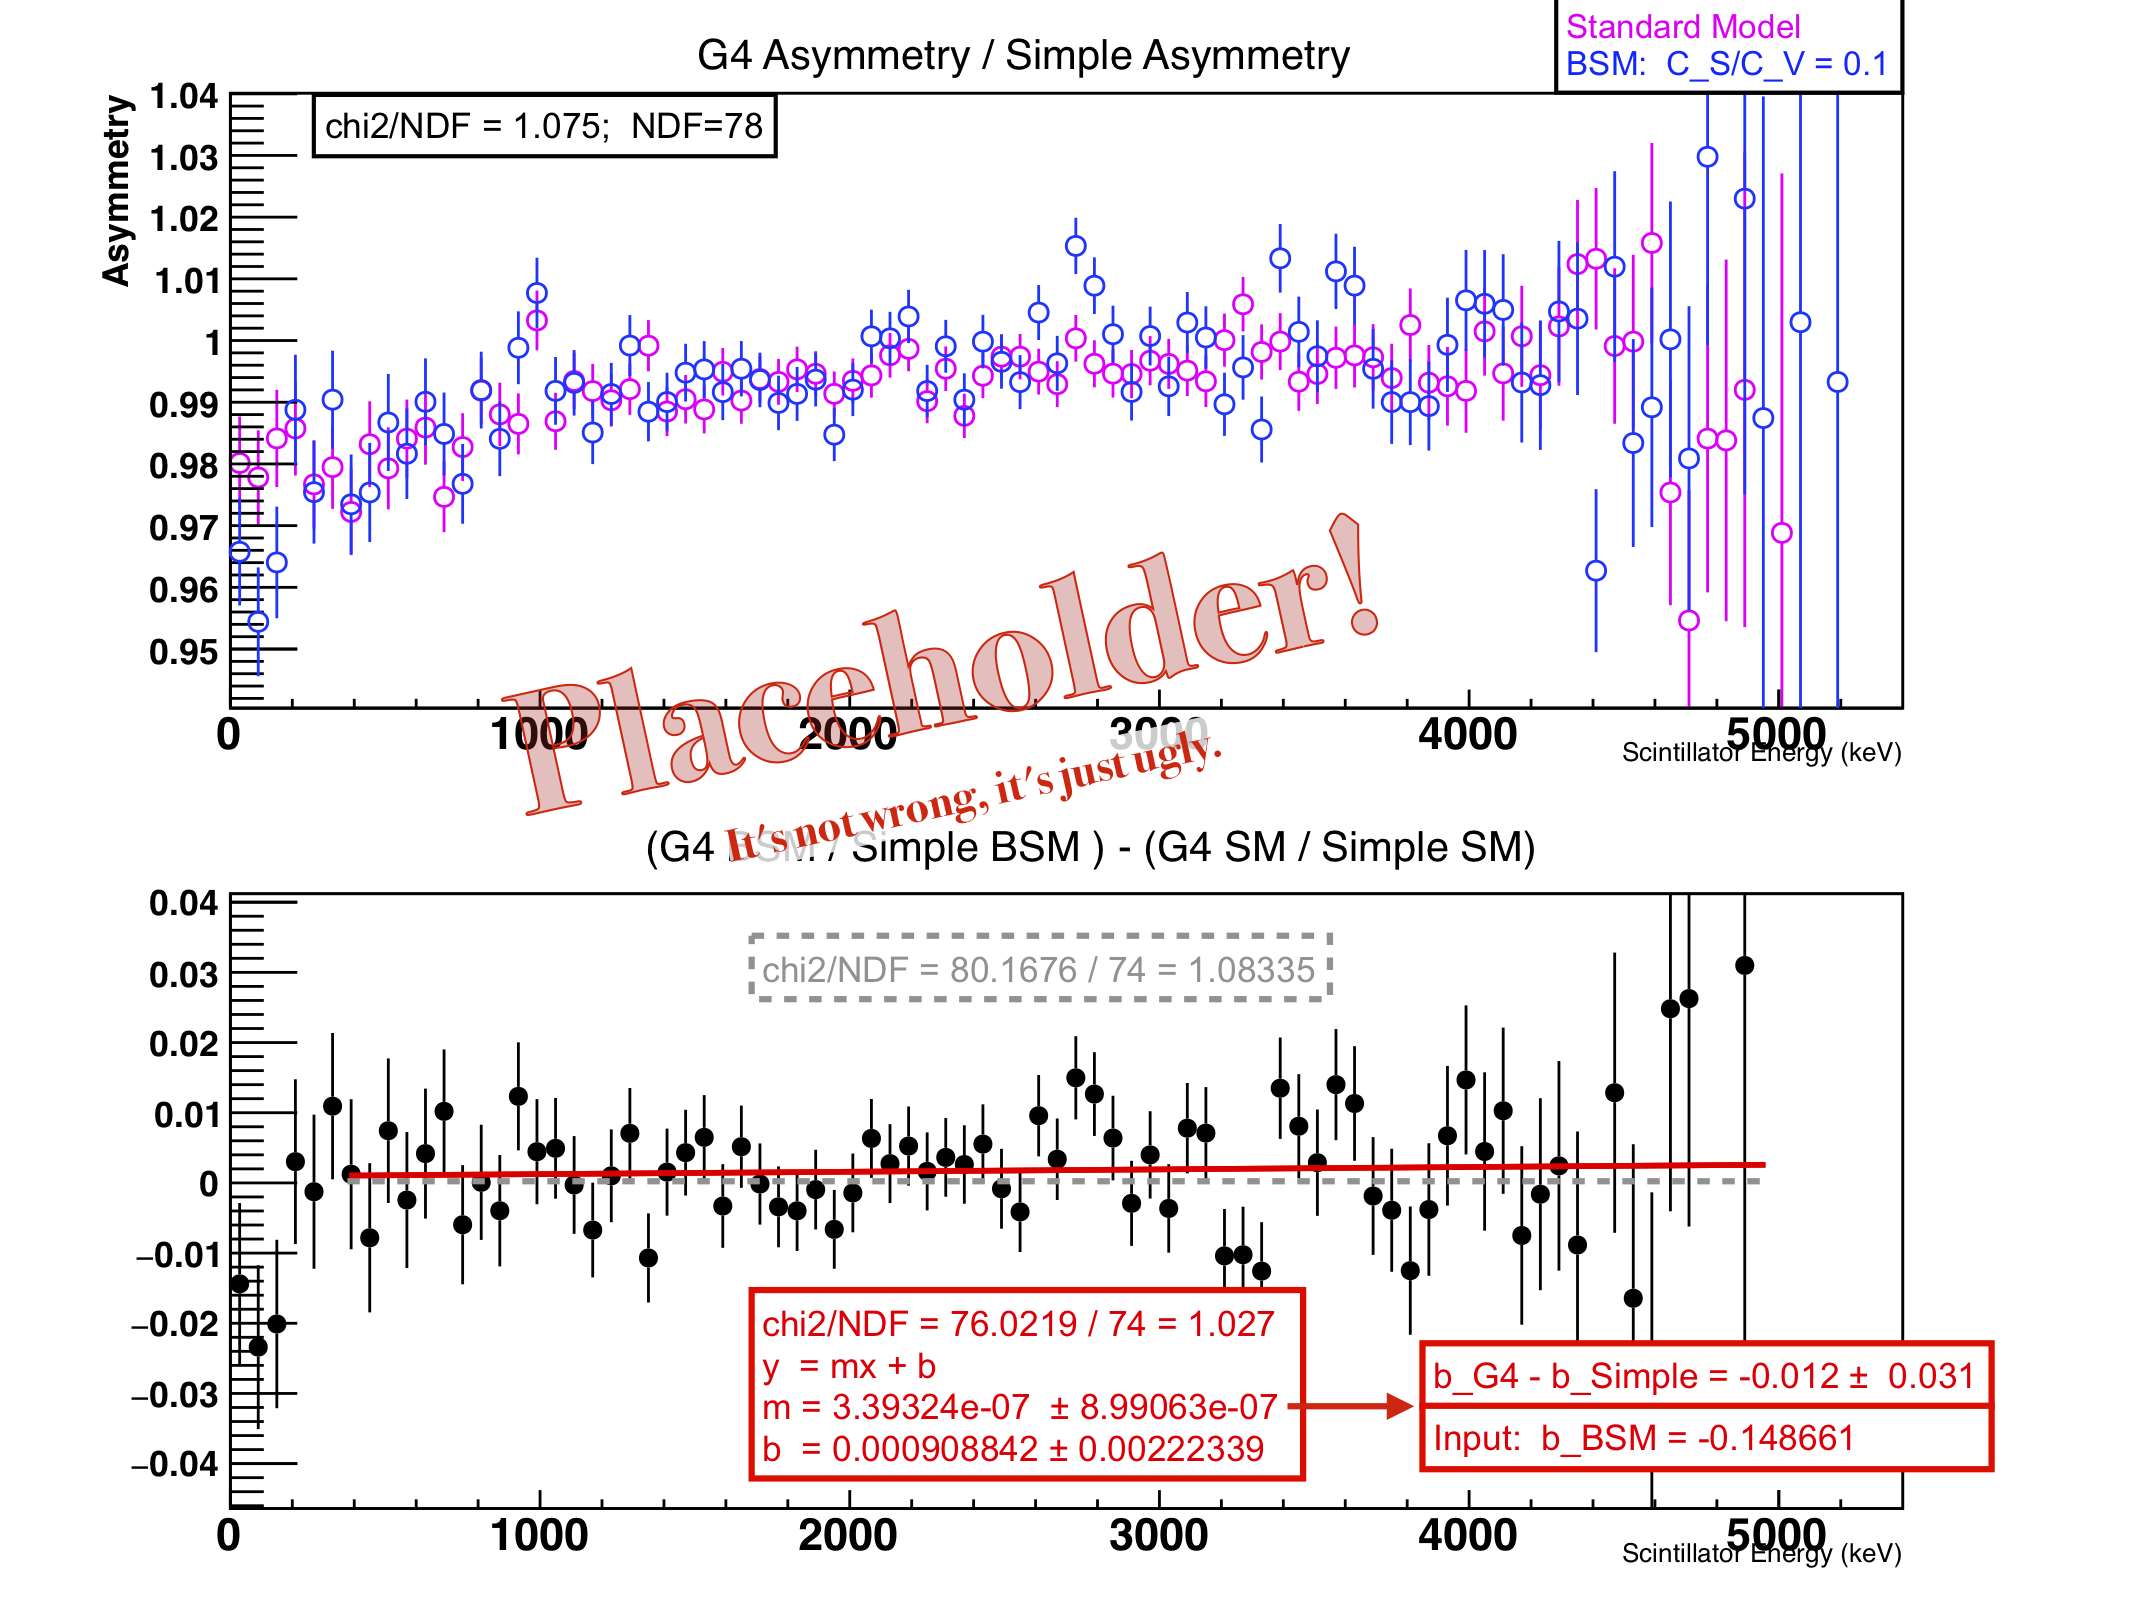
\includegraphics[width=.999\linewidth]
    	{Figures/LineshapeDemo_prelim.png}
    	\caption[Lineshape Comparison]{I'm not actually sure if this picture shows what I want it to.  The point is, if I apply this rough lineshape to stuff that I SimpleMC-ed, then I can evaluate that way various systematic effects that would be time-consuming to actually simulate with G4.  This picture is  *supposed* to be a demonstration that this approach actually works... }	
    	\label{fig:lineshape_demo}
    \end{figure}
	
	\subsection{The Math-Specifics}
	I'll write down the specific functions I'm using, and the parameter values I'm using.  (Maybe this should go in an appendix instead?)  I'll describe the adjustments I make to the spectrum so that it can work even for the dataset where the scintillators' resolutions have changed.
	
	\subsection{The Results -- Things That Got Evaluated This Way}
	As it turns out, only cloud parameters were evaluated this way. \aside[color=jb]{JB:  so it's still critical to write down more of the lineshape work.}
Trap position, size, sail velocity, temperature.  But then we varied the lineshape anyhow, to account for G4 doing a bad job of modelling the bremsstrahlung (sp?).
	%Thicknesses of the SiC mirror, the Be foil, and the DSSD.  Scintillator calibration.  
	\note[color=jb]{JB:  yes, brems strahlung is 'braking radiation' so gets 2 ss's. 
the lineshape tail in any scintillator also includes backscattered events -- we are not claiming the 2-pixel cut is complete}
	
	    \begin{figure}[h!!]
    	\centering
    	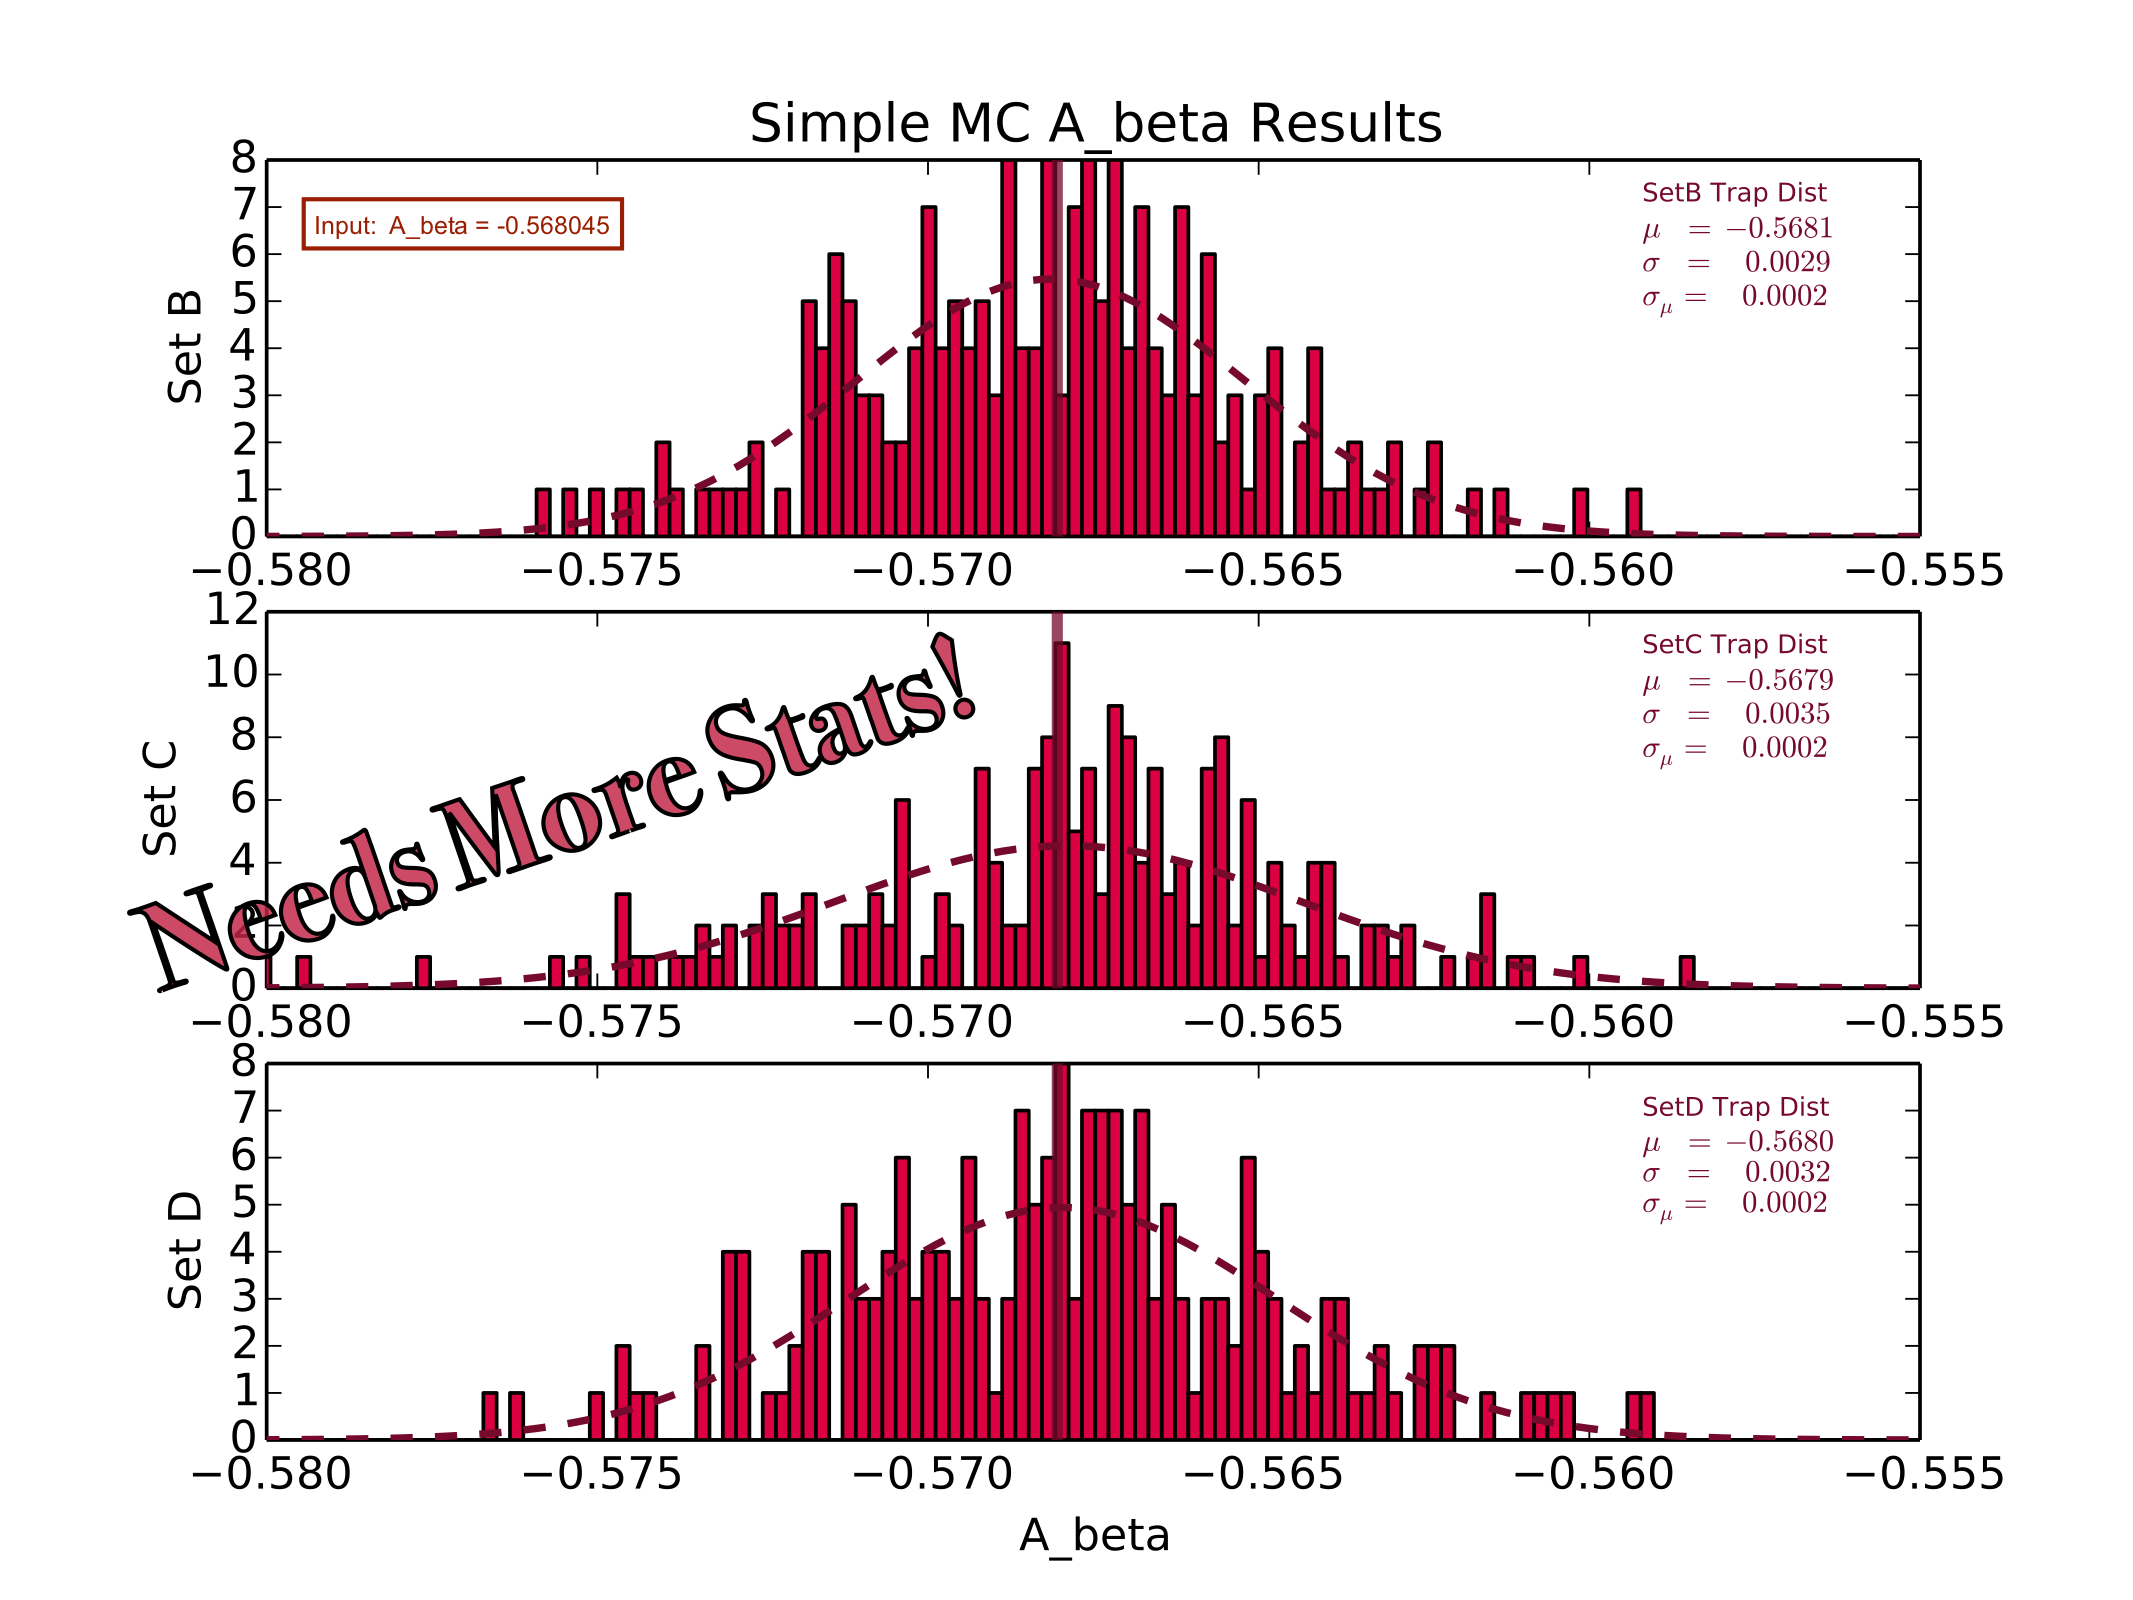
\includegraphics[width=.999\linewidth]
    	{Figures/Position_Err_Abeta_prelim.png}
    	\caption[$\Abeta$ Position Error]{Estimated uncertainty in $\Abeta$ resulting from uncertainty and variation in the cloud parameters.  Evaluated by the lineshape reconstruction method.}	
    	\label{fig:Abeta_position_err}
		\end{figure}

	    \begin{figure}[h!!]
    	\centering
    	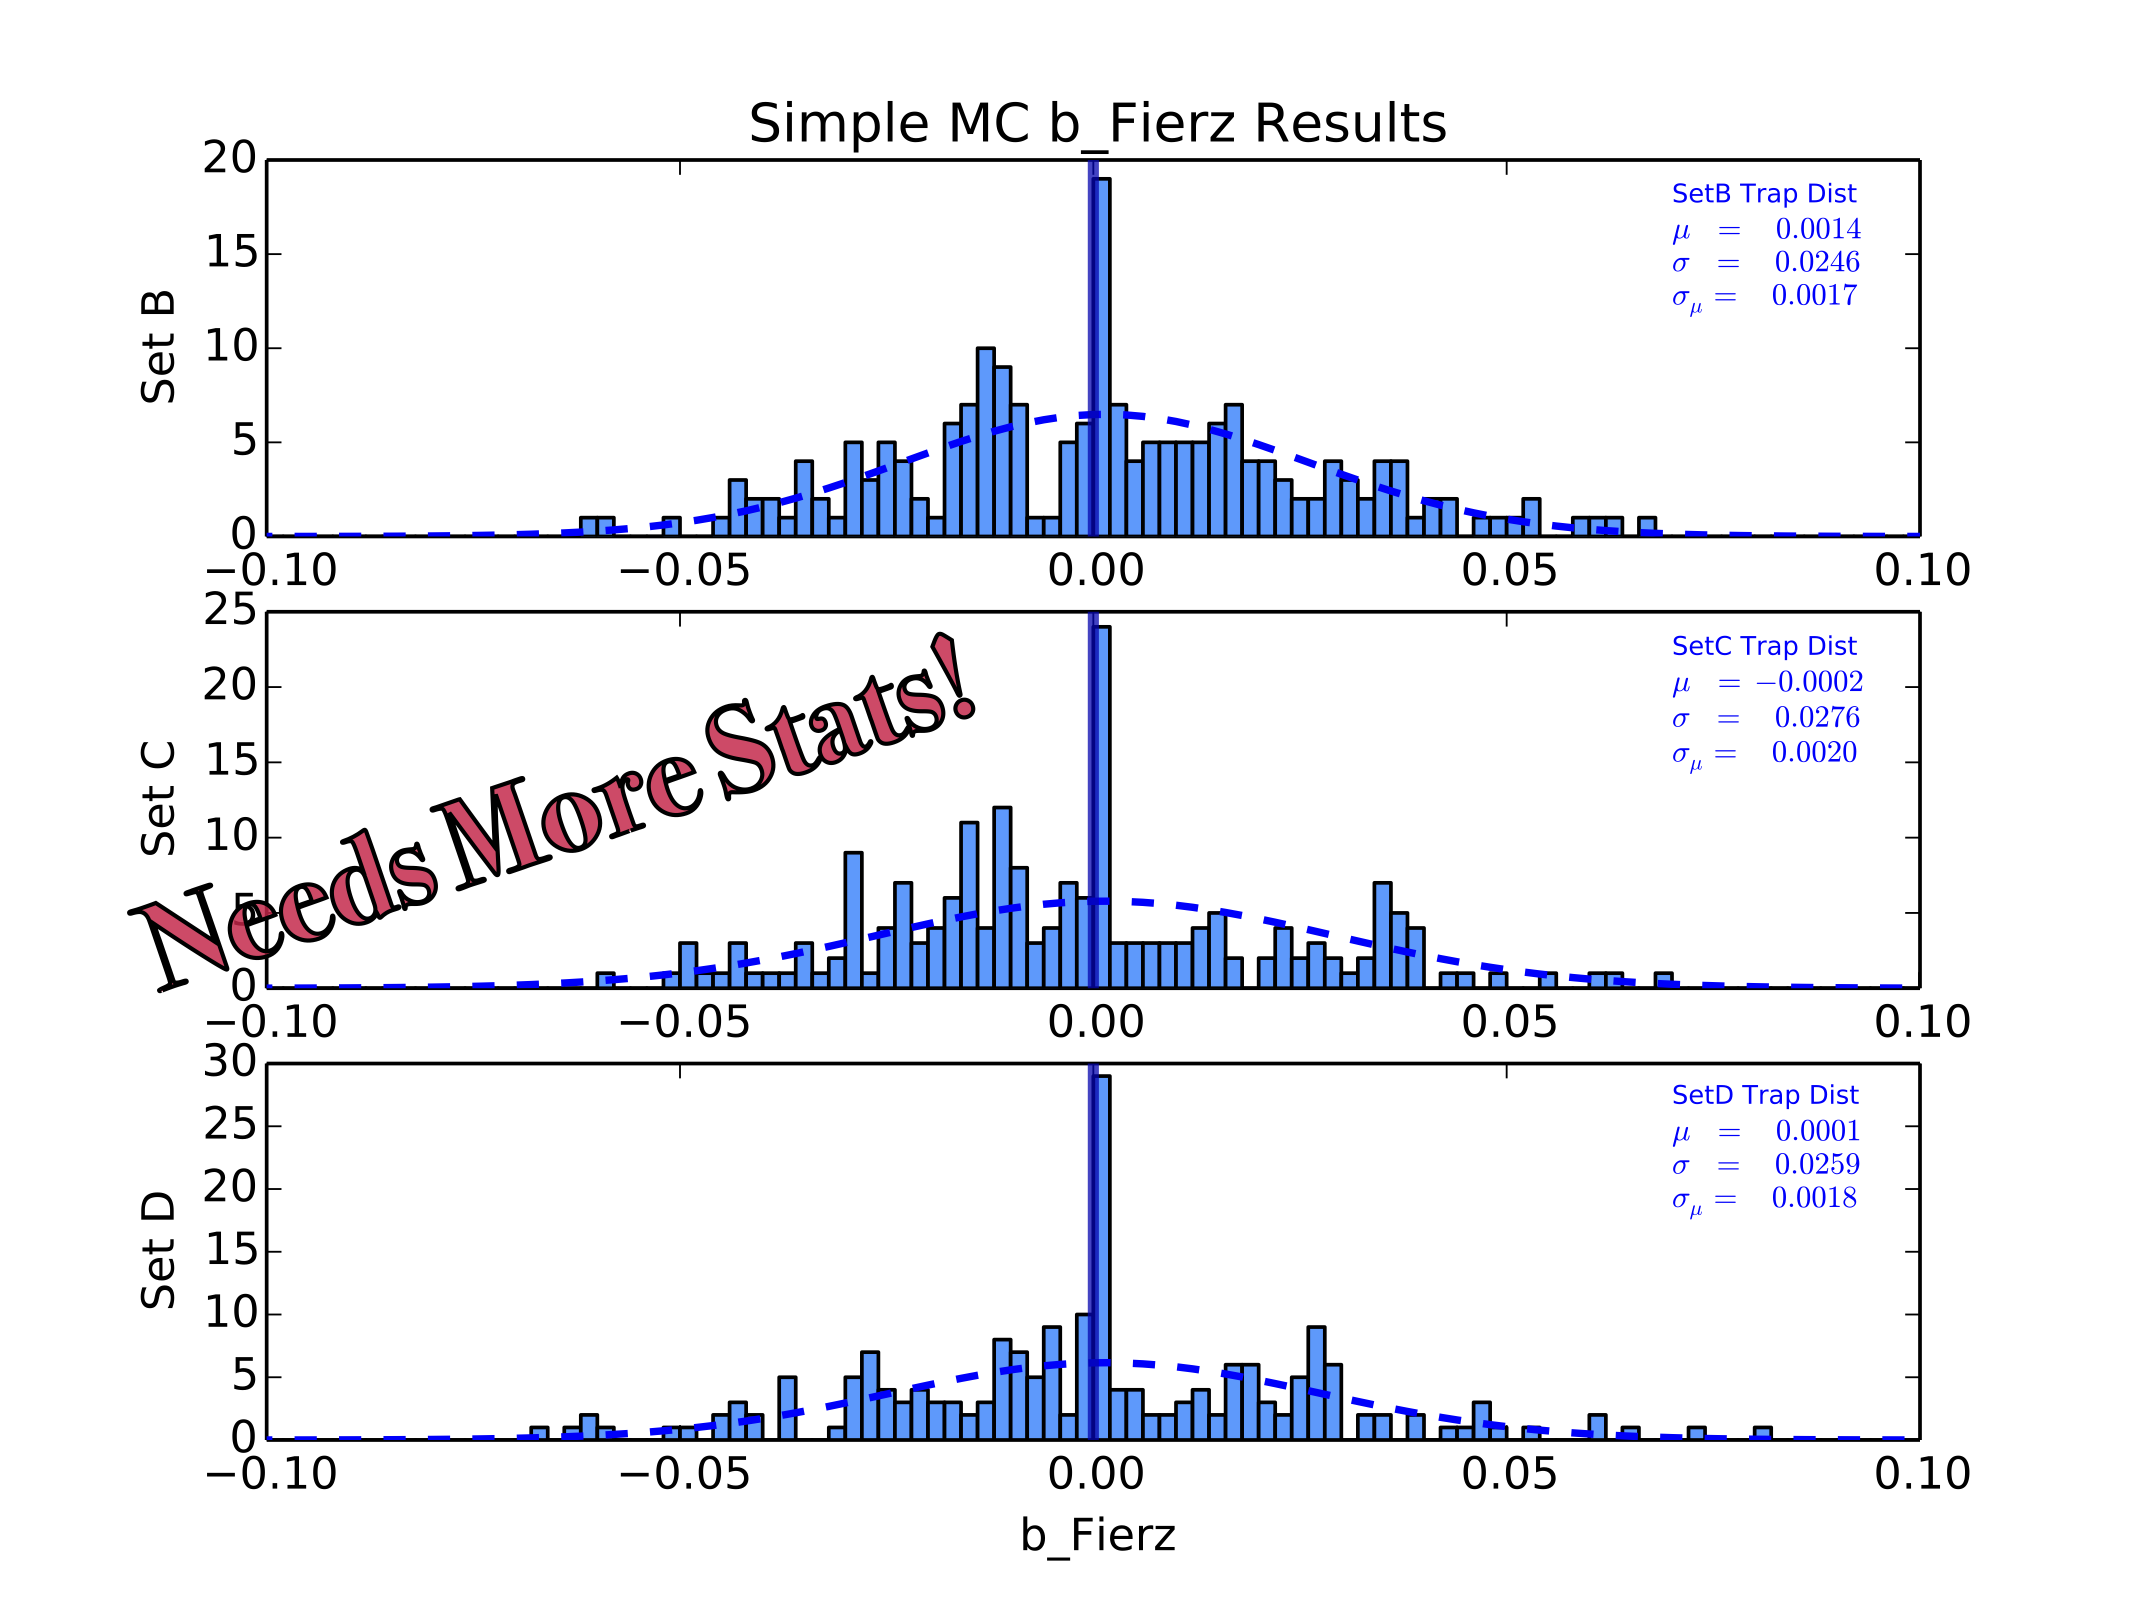
\includegraphics[width=.999\linewidth]
    	{Figures/Position_Err_bFierz_prelim.png}
    	\caption[$\bFierz$ Position Error]{Estimated uncertainty in $\bFierz$ resulting from uncertainty and variation in the cloud parameters.  Evaluated by the lineshape reconstruction method.}		
    	\label{fig:bFierz_position_err}
		\end{figure}

	
	\subsection{The low-energy tail uncertainty, and what it does}
	Bremsstrahlung.  It does Bremsstrahlung.
%	\note[color=jb]{JB:  ``I will write this up better soon."  (I think he already did that)}
\note[color=jb]{ Here is Subsection 9.5.5 ``The low-energy tail uncerainty, and what it does'' complete.  There should be no figure.
\\
Direct quote from John follows in the next two paragraphs.  Maybe I should paraphrase, but it's so nicely written! }

\comment{
This subsection has the collaboration's evaluation of the uncertainty from
the scintillator detector's lineshape tail.
The energy from a monoenergetic beta is not always fully absorbed
in a plastic scintillator.
Although most backscattered betas are vetoed by the DSSD,
some produce bremsstrahlung photons,
and these frequently escape low-Z plastic scintillator-- all cross-sections
are known to high accuracy, but there is always uncertainty entailed in  the
MC implementation.
This lineshape tail will then effectively move events from higher to lower measured
energy, artificially altering the lower-energy asymmetries and mimicking the effects of a
Fierz term.

Since this detector effect is difficult to disentangle from the other scattering
effects off volumes,
the collaboration adds a linear function down to zero for the tail to
a Gaussian for the peak,
with linewidth varying by photon statistics~\cite{clifford}.
The convolution of this simple detector response function with v/c then scales the
centroid MC, with the lineshape tail varied by $\pm$10\% of its value,
a generic uncertainty accepted by the community for MC electromagnetic simulations.
The fit $b_{\rm Fierz}$ centroid changes by $\pm$ 0.0076, summarized
as the 0.008 ``Low Energy Tail'' in the systematics table at the start of this chapter.
Compared to other uncertainties of the present data set,
this is small enough that the accuracy of this estimate is adequate.
}

%\note[color=jb]{End direct quote paragraphs from John.}

%\section{Summary of Data Collected}
%\missingfigure{TBH, the thing that's missing is a table, not a figure.  Needs a table full of systematic errors.  And maybe statistical errors?  wev.}
%\note{Needs an error budget table.  Because of course it fucking does.}





%%%% --- * --- %%%%	
% !TEX root = ../thesis_main.tex



\clearpage	
\chapter{Results}
\label{results_chapter}

\section{Measured Limits on $b_{Fierz}$, $C_S$, $C_T$}
	%\\*
	Results go here, with measured limits described and quantified in all formats anyone could ever care about.
	
\begin{figure}[h!!!t]
	\centering
	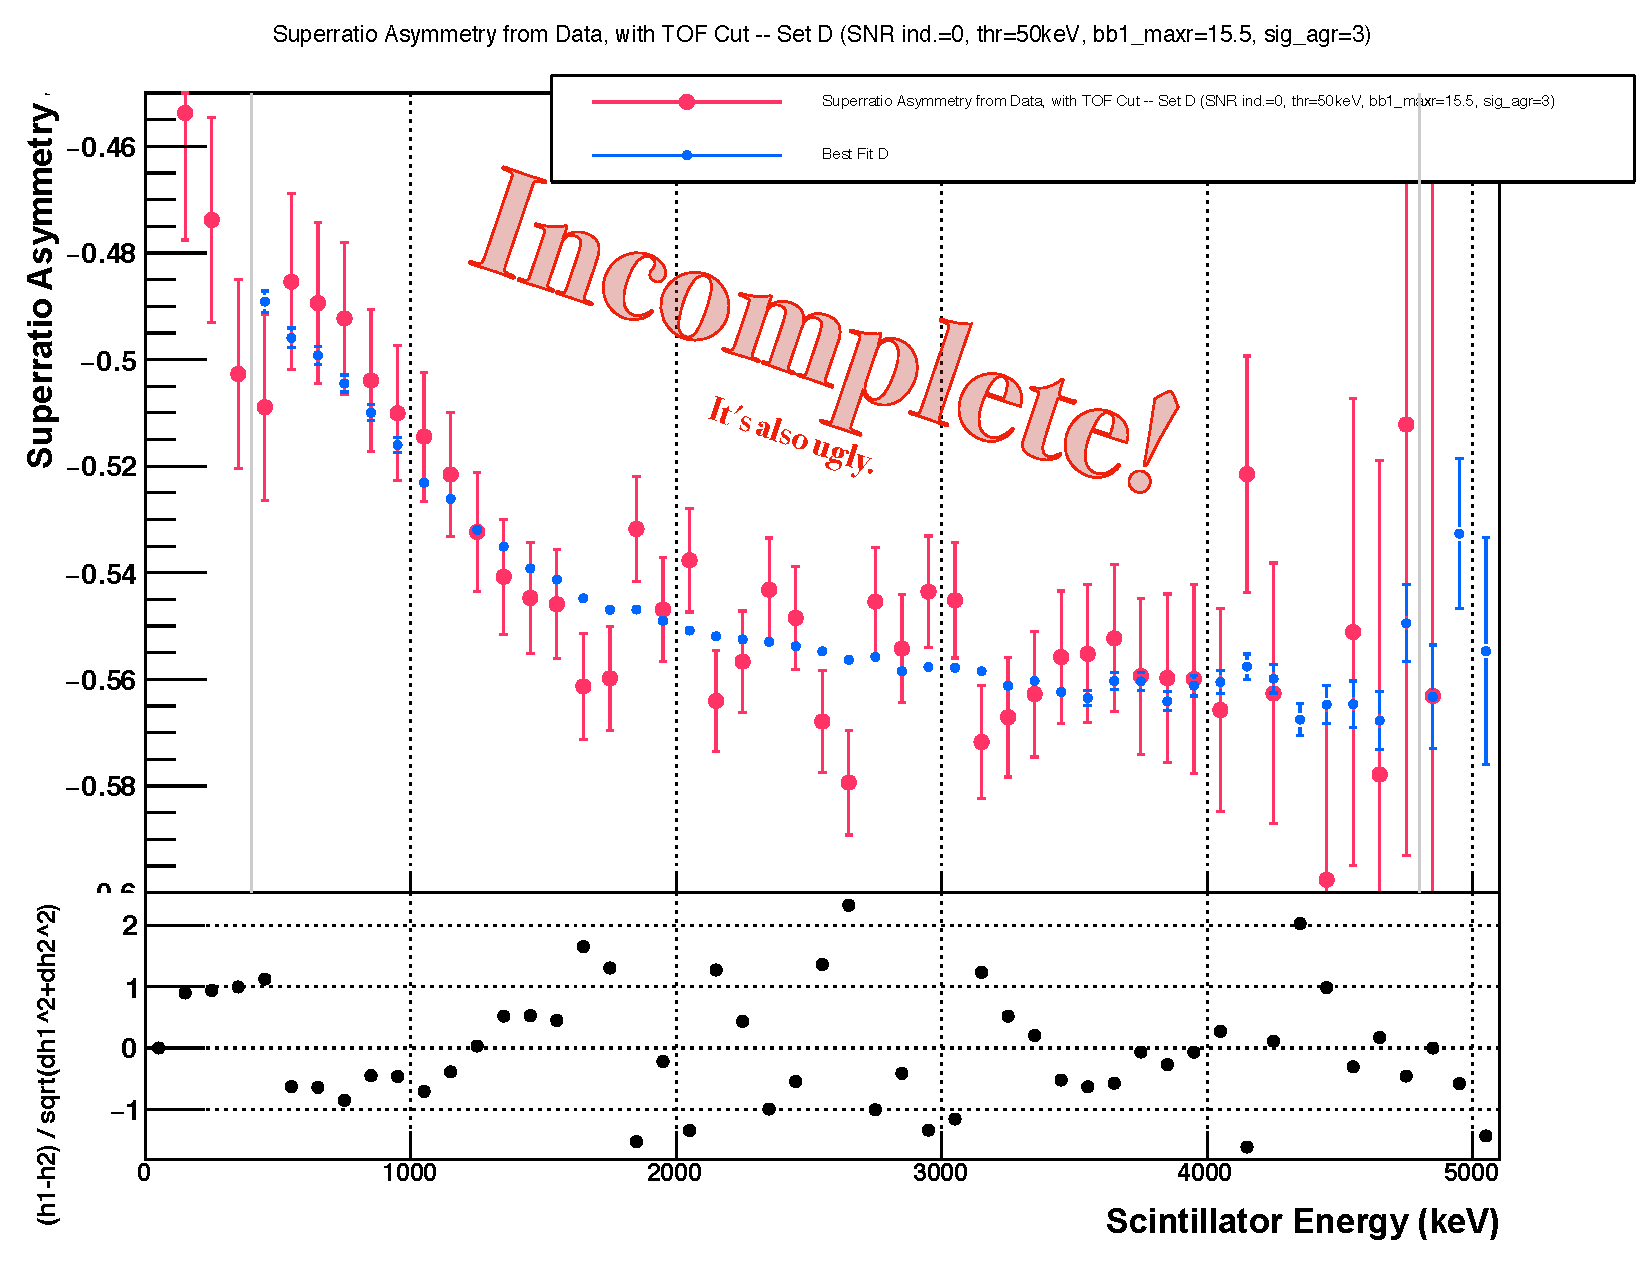
\includegraphics[width=.999\linewidth]
	{Figures/AsymmetryAndResiduals.pdf}
	\caption{A superratio asymmetry from the data, and the best fit from simulations.}	
	\label{fig:asymmetry}
\end{figure}
	
	
\begin{figure}[h!!!t]
	\centering
	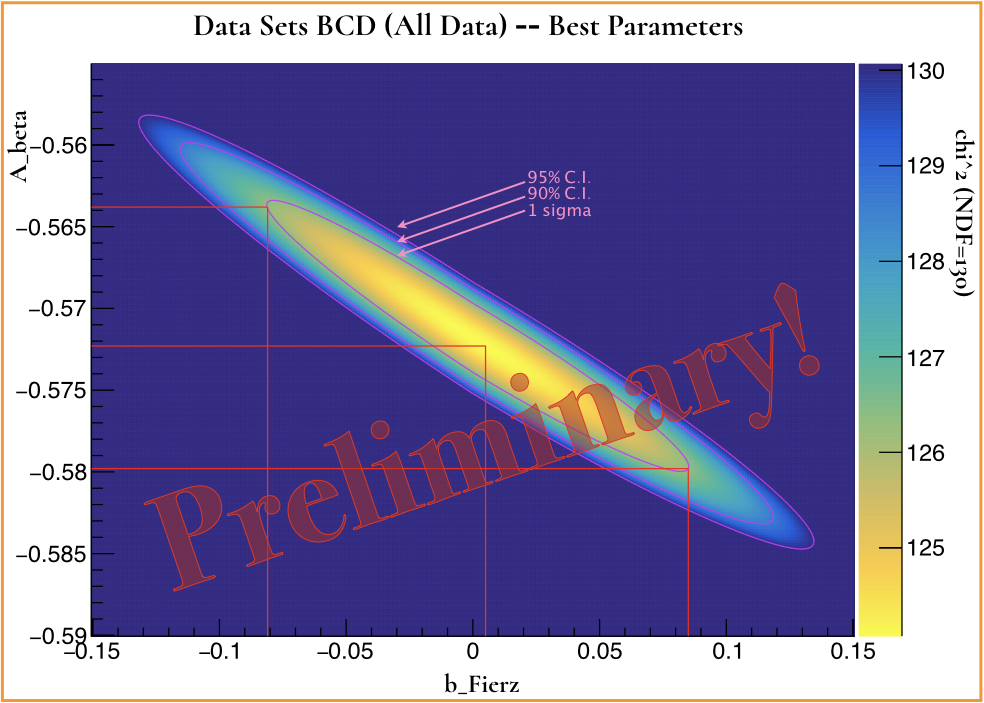
\includegraphics[width=.999\linewidth]
	{Figures/Abeta_bFierz_2D_prelim.png}
	\caption{Some results.  I'll want to show at least one of these things.  Probably show a separate one for each runset, actually.}	
	\label{fig:2d_results_bcd}
\end{figure}

\section{Discussion of Corrections and Uncertainties}
	...
	
\section{Relation to Other Measurements and New Overall Limits}
	%\\*
	In which I'll show exclusion plots and write down new limits, combining my result with results from the literature.















